\documentclass[English, Lau, oneside]{sapthesis}
%\usepackage{hyperref}
\usepackage{microtype}
\usepackage[english]{babel}
\usepackage[utf8]{inputenx}
\usepackage{graphicx}
\usepackage{float} % Include the float package
\usepackage{skmath}
\usepackage{amsmath, xparse}
\usepackage{wrapfig}
\usepackage{float}
\usepackage{tikz}
\usepackage{amsmath,amssymb}
\usepackage{sidecap}
\usepackage{xcolor}
\usepackage{gensymb}
\usepackage{caption}
\usepackage{tabularx}
\usepackage{geometry}
\usepackage[utf8]{inputenx}
\usepackage{indentfirst}
\usepackage{microtype}
\usepackage[utf8]{inputenc}
\usepackage{graphicx}   % Per includere immagini
\usepackage{subcaption} % Per creare sottografie
\usepackage{amsmath}    % Per formule matematiche, se necessario
\usepackage[italian]{babel}
\usepackage{siunitx}
\DeclareMathOperator\erf{erf}
\usepackage{hyperref}
\usepackage{amsmath}
\usepackage{tikz}
\usetikzlibrary{arrows.meta}
\usepackage{csvsimple}
\usepackage{subfig}
\usepackage{placeins}
\usepackage{subcaption}
\usepackage{xfrac}
\usepackage[makeroom]{cancel}
\usepackage{verbatim}
\usepackage{ gensymb }
\usepackage{tikz}
\usetikzlibrary{arrows.meta, positioning}
\usepackage{ longtable }
\usepackage{geometry}
\usepackage{eucal}
%\usepackage{hyperref}
\usepackage{braket}
\usepackage{bbold}
\usepackage[hidelinks]{hyperref}
\usepackage{indentfirst}
\usepackage{microtype}
\usepackage{amsmath}
\usepackage{siunitx}
\usepackage{hyperref}
\usepackage{subcaption} % per subfigure
\usepackage{tikz}
\usetikzlibrary{arrows.meta, positioning}
\usepackage[titles]{tocloft}


%\usepackage{chemformula}
%\usepackage{setspace}
%\usepackage{yfonts,color}
%\usepackage{siunitx}
%\usepackage{comment}
%\usepackage{multirow}
%\usepackage{varioref}
%\usepackage[bottom]{footmisc}
%\usepackage{wrapfig}
%\usepackage{float}
%\usepackage{type1cm}
%\usepackage{chngcntr}
%\onehalfspacing
%\counterwithout{footnote}{chapter}
\usepackage{hyperref}
\usepackage{hyperref}
\hypersetup{
			hyperfootnotes=true,			
			bookmarks=true,			
			colorlinks=true,
			linkcolor=red,
                        linktoc=page,
			anchorcolor=black,
			citecolor=red,
			urlcolor=blue,
			pdftitle={La natura particellare della materia oscura},
			pdfauthor={Enrico Bignozzi},
			pdfkeywords={thesis, sapienza, roma, university}
 }


\hypersetup{pdftitle={Sapthesis class example},pdfauthor={Francesco Beccari}}

% Remove in a normal thesis
\usepackage{lipsum}
\usepackage{curve2e}
\definecolor{gray}{gray}{0.4}
\newcommand{\bs}{\textbackslash}

% Commands for the titlepage
\title{Protein response in equilibrium and out of equilibrium conditions}
\author{Bignozzi Enrico}
\IDnumber{1855163}
\course{Corso di Laurea Magistrale in Fisica}
\courseorganizer{Facoltà di Scienze Matematiche, Fisiche e Naturali}
\AcademicYear{2025}
\copyyear{}
\advisor{Fabio Cecconi}
\coadvisor{}
\authoremail{bignozzi.1855163@studenti.uniroma1.it}

%\examdate{16 April 2013}
%\examiner{Prof. Nome Cognome}
%\examiner{Prof. Nome Cognome}
%\examiner{Dr. Nome Cognome}
%\versiondate{\today}
\begin{document}
\maketitle
\addcontentsline{toc}{chapter}{Index}
\tableofcontents

%\begin{abstract}

%\end{abstract}

%\begin{acknowledgments}
    
%\end{acknowledgments}

\dedication{}

\newpage
\null
\thispagestyle{empty}
\newpage



\chapter*{Introduction}
\noindent In this thesis we will study the allosteric mechanism of a protein in and out of equilibrium conditions.\\
Allostery is the phenomenon by which the binding of an effector molecule to a specific site on a protein, known as the allosteric site, induces a conformational change that affects the functional activity of a distant site, typically the active site. This interaction does not occur through direct binding between the sites but rather through a series of internal network changes within the protein structure, which transmits the signal and ultimately modulates its function.
We want to understand it in a quantitative way, using causal indicators for studying the propagation of the signal along the structure of the protein.
\begin{figure}[H]
    \centering
    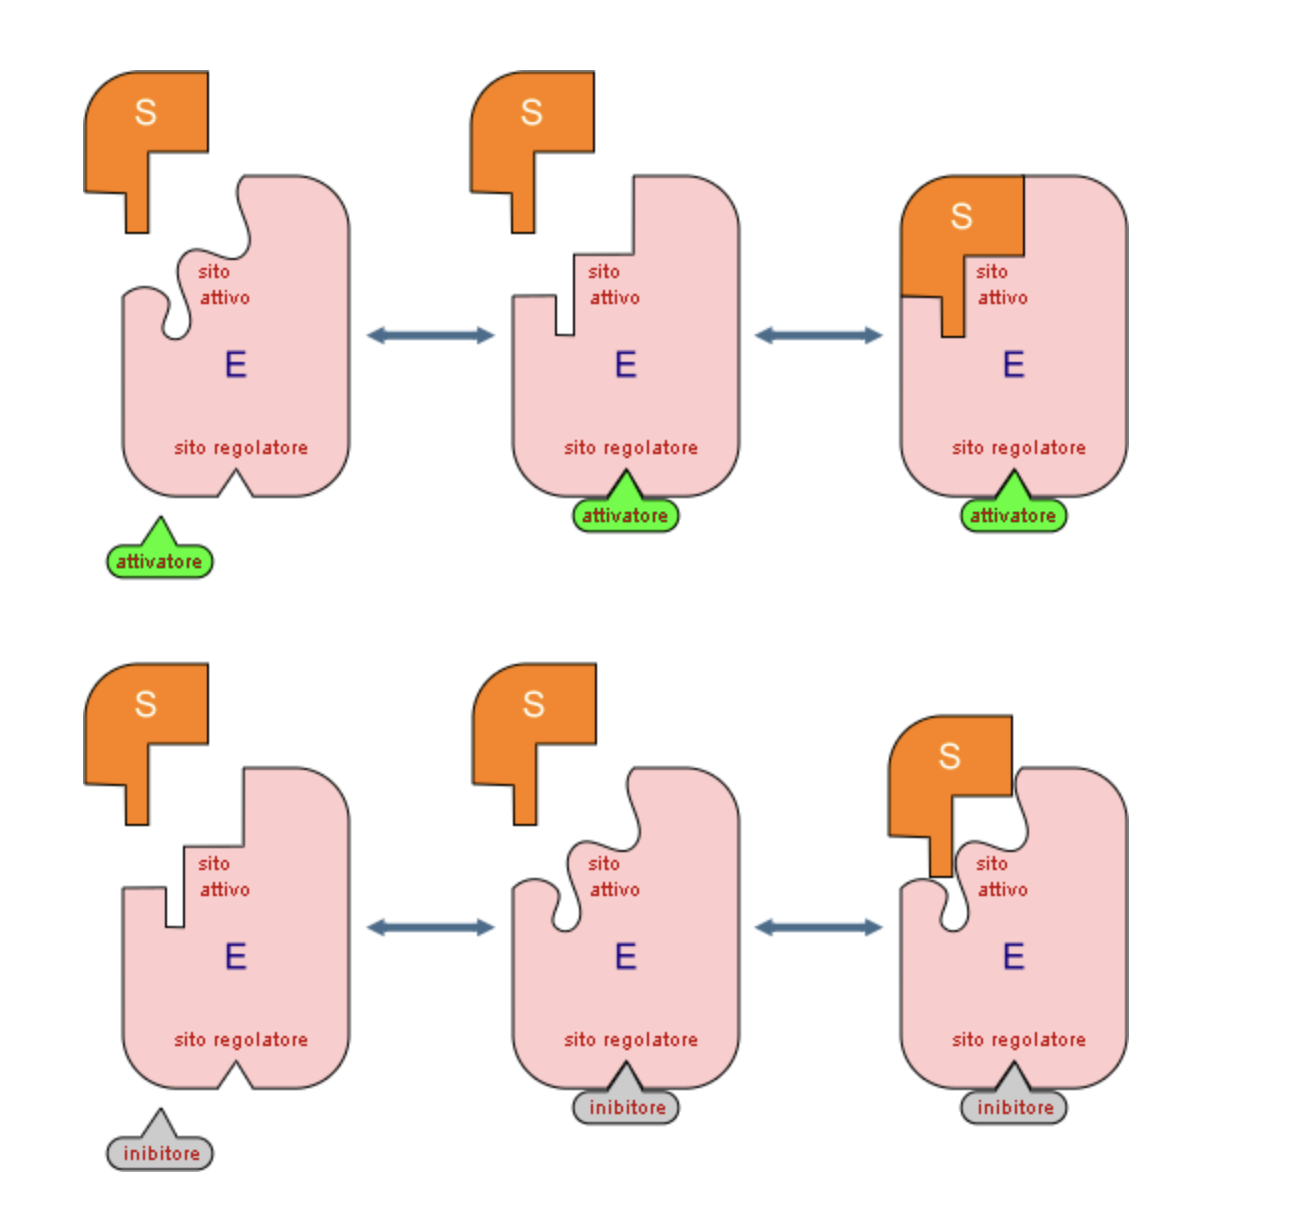
\includegraphics[width=1\textwidth]{/Users/enrico/PROTEINS/tesi/immagini_tesi_ingelse/Screenshot 2024-12-17 at 10.57.30.png}
    \caption{Schema of allosteric mechanism with active and allosteric site}
\end{figure}


\paragraph{Chapter 1: Protein Structure} \\
In the first chapter we will explain what a protein is and the basic concept about it.

\paragraph{Chapter 2: Relation structure-function-dynamic in proteins} \\
In the second chapter we will expose the importance relation structure-function-dynamic in proteins. 
It is very important the geometry structure of the protein and one of my aim is to show how much of the protein's behavior can be explained only from its geometric structure.
In fact it comes from years and years of evolutionary optimization process.

\paragraph{Chapter 3: Relation structure-function-dynamic in proteins} \\
In the third chapter we will study the normal modes and the guassian network model as a model to trehat the protein as a network of interactions between atoms.
This is a very useful model to study the protein's behavior and in particular the allosteric mechanism, in which model the geometric structure is the only important factor to explain the protein's behavior.
Finaly we will introduct the allosteric mechanism and we will see specifically in 3LNX protein, where we expect that a signal from an allosteric site can propagate to the hydrophobic pocket, that is the active site of the protein, avoiding the protein to catch a ligand.\\


\paragraph{Chapter 4: Causality indicators} \\
We will study also the causality indicators, that are a powerful tool to study the propagation of the signal along the protein's structure and to undestrand the allosteric mechanism.
We will present the covariace, the response and the transfer entropy as causal indicators.
\paragraph{Chapter 5: Causality indicators} \\
We will show the result and how good this model explain the allosteric behavior of the protein.

\vspace{1cm}








\chapter{Proteins}
\section{Structures of Amino Acids and Proteins}
\noindent 
Our objective is to explore how the amino acids making up the protein interact with each other.\\
Specifically we aim to comprehend allsoteric mechanisms .
First we need to understand what is a protein.\\
Proteins are composed of a sequence of amino acids that fold into a three-dimensional structure which determines their function. \\
Some of the functions include: 
accelerating chemical reactions by lowering the activation energy (Catalysis);
regulating signal transduction and gene expression (Regulation and Signaling); 
the transport of molecules through cell membranes (Transportation);
and the providing of mechanical support and structural integrity to tissues (Structural roles).\\
But what is an amino acid?\\
Amino acids are the building blocks of proteins, they are organic molecules which contain a central carbon atom (\(\alpha\)-carbon) bonded to 
an amino group (-NH2), a carboxyl group (-COOH), a (\(R\)-Group), that changes from amino acid to amino acid, and finally to a hidrogen atom.\\
The \(R\)-group is particularly important because it determines the chemical properties of the amino acid, such as whether it is hydrophilic, hydrophobic, acidic, or basic.\\
\begin{figure}[H]
    \centering
    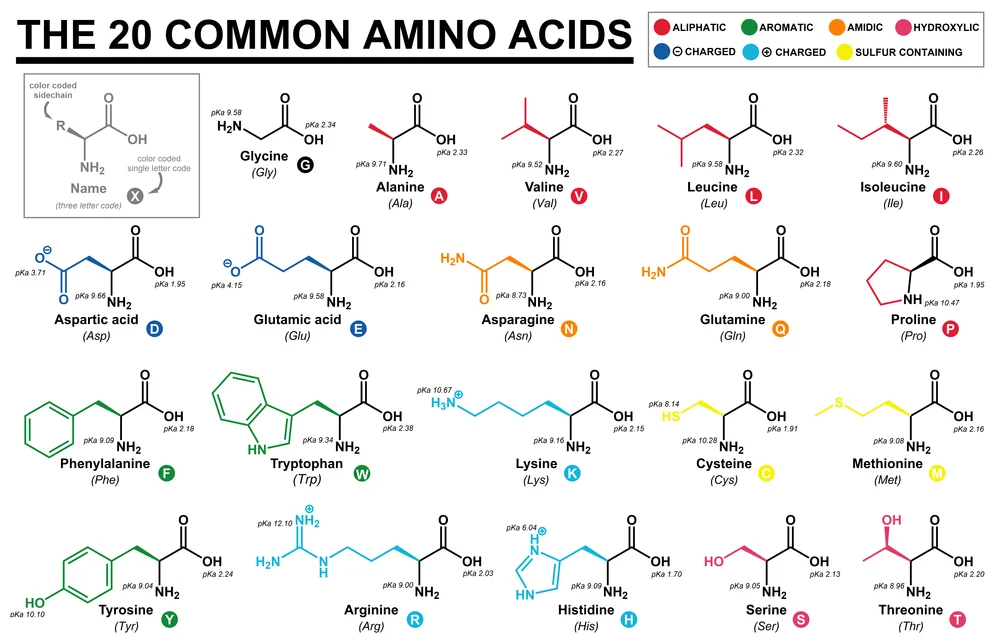
\includegraphics[width=1\textwidth]{/Users/enrico/PROTEINS/tesi/immagini_tesi_ingelse/ammino.png}
    \caption{Amino Acids}
\end{figure}
\newpage





The structure of a protein is divided into four levels which are very important for understanding its function.\cite{ref4}\\
The primary structure is a linear sequence of amino acids in a protein chain, held together by peptide bonds.\\ 
Instead the secondary structure represents the local folding of the protein chain in patterns.
In this work we will focus in the following secondary structures in particular on alpha-helix, beta-sheet and loop regiones.\\ 
The first two are ordered patterns in which every amino acid is connected with the other amino acid in a specific way, the loop instead is a disordered region of the protein.\\
In particular alpha-helix is a right-handed spiral structure stabilized by hydrogen bonds between the NH and CO groups of amino acids separated by four residues, while beta-sheet is a structure in which the amino acids are connected by hydrogen bonds in a zigzag ( parallel or antiparallel) pattern
and finally the loop is a region of the polypeptide chain that connect other secondary structures.\\
The tertiary structure describes the three-dimensional folding of the entire protein molecule 
and quaternary structure consist of more than one polypeptide chain that are arranged and interact with each other to form the functional protein complex.
Obviously all these structures arise from the interactions between the amino acids that compose the protein. 
Following we will see our model of interactions between the amino acids.

\begin{figure}[H]
    \centering
    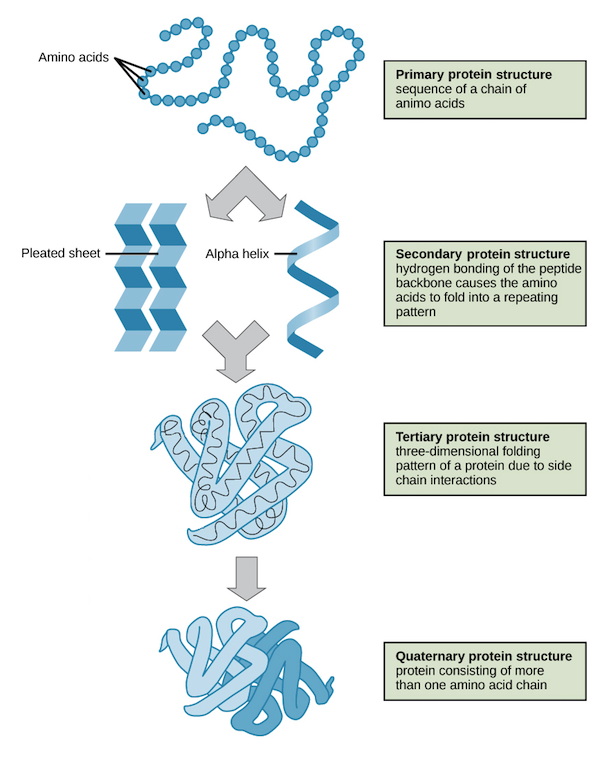
\includegraphics[width=0.5\textwidth]{/Users/enrico/PROTEINS/tesi/immagini_tesi_ingelse/71225d815cafcc09102504abdf4e10927283be98.png}
    \caption{Structures}
\end{figure}



\newpage

\chapter{Structure-Function-Dynamic Relationship in Proteins}

\section{Relation between Structure, Function, and Dynamics in Proteins}
\noindent The fundamental idea is that a protein's structure dictates its function. This structure governs the interactions between amino acids within the protein. If proteins were random aggregates of amino acids, they would not be able to perform their specific functions.\\
In fact the evolution optimizes the protein’s utility function, creating a structured arrangement that is not random.
Finally this structure determines how signals propagate along the protein.\\

Proteins rely heavily on their ability to change shape in order to carry out their functions effectively; this involves more, than movement but also includes interactions between distant areas within the protein structure that are crucial for important biological processes, like attaching to other molecules or binding with ligands.\\ 
Proteins can undergo variations by either moving their acids around a central point or interacting with other molecules to alter their shape. \\
Therefore we propose (which is the assumption of this study) that the structural shape of the protein itself reveals a lot, about how the allosteric process works.\\
So we're going to create a model that relies completely on structure and try to clarify every detail.  Obviously, there are many additional factors that we must consider to accurately model the behavior of proteins.\\
Obviously, there are many additional factors that we must consider to accurately model the behavior of proteins.\\

\newpage
\section{Allostery}
\noindent Allostery, derived from the Greek \textit{allos} (other) and \textit{stereos} (structure), is the phenomenon of a change in protein structure caused by the transmission of a signal from one site to another.\cite{ref5}  
More precisely, allostery occurs when the interaction of a molecule (effector) with a specific site on a protein, known as the allosteric site, induces a conformational change that influences the functional activity of another site, usually the active site.
This process does not involve direct interactions between the two sites but occurs through changes in the protein’s internal network.

There are two key types of allostery that govern how proteins regulate their functions: conformational allostery and dynamic allostery. 
While both are based on the transmission of a signal through the protein’s structure, they differ in the mechanism of action.
Conformational allostery involves a structural change in the protein that occurs when an effector molecule binds to an allosteric site. This binding induces a distinct, often visible, shift in the protein’s shape, such as a transition from a less active (relaxed) state to a more active (tense) state. 
This structural shift propagates through the protein, modifying its function.
Mathematically, conformational allostery can be described in terms of the population of microstates of the protein, as well as the equilibrium constant between different states, such as:

\[
L = \frac{[T]}{[x]}
\]

where \([T]\) and \([x]\) represent the relative concentrations of the two conformational states, relaxed and tense, and \(L\) describes the equilibrium constant between them.

\begin{figure}[h]
    \centering
    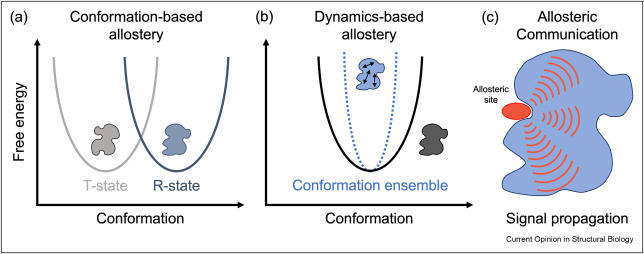
\includegraphics[width=\textwidth]{/Users/enrico/PROTEINS/tesi/immagini_tesi_ingelse/1-s2.0-S0959440X23002117-gr1.jpg}
    \caption{Schematic representation of allostery: the interaction with an allosteric effector (site A) induces a conformational change that affects a distant site (site B).}
    \label{fig:allostery_dynamics}
\end{figure}
In contrast, dynamic allostery is based on fluctuations and flexibility within the protein’s structure. Instead of a fixed structural change, dynamic allostery involves the modulation of the protein’s internal dynamics, where small oscillations or fluctuations in the protein’s atomic structure propagate across its network of interactions. These dynamic changes influence the protein's ability to bind ligands or interact with other biomolecules.

Dynamic allostery often does not result in obvious structural shifts but involves subtle changes in the protein's flexibility. These changes are essential for the protein’s function, as they allow the protein to respond to environmental signals without requiring large-scale conformational changes.

Both conformational and dynamic allostery rely on causal mechanisms—specifically, how an effector molecule's binding event at one site causes changes at a distant site. However, the distinction lies in how these signals are transmitted.\\
In conformational allostery, this is typically achieved through a direct structural change, while in dynamic allostery, it occurs via shifts in the protein's internal network dynamics, often without a distinct change in overall structure.\\
To fully grasp how proteins achieve their functional structure, it is crucial to explore the causal mechanisms behind these conformational and dynamic changes. Understanding how the signal propagates between amino acids and how localized binding events can influence distant regions of the protein is essential for studying allosteric mechanisms. This propagation of information is key to explaining how localized interactions can regulate the overall function of the protein, thus facilitating complex biological processes.
This understanding is especially important in drug development, where manipulating these allosteric sites and their causal mechanisms can lead to the creation of more effective therapeutic strategies.

A classcial exemple of allostery is the HIV protease.\\
The HIV protease is a key enzyme in the maturation of the HIV virus. After infecting a host cell, the virus produces a long chain of amino acids that must be cleaved into smaller peptides to form a functional, infectious protein. This process is regulated by allosteric mechanisms, where the binding of specific molecules to the protease induces conformational changes, affecting its ability to cleave the peptide chain and thus regulating viral maturation.

These cuts are essential for the virus to assemble the amino acids and mature into an infectious form. Therefore, inhibiting the protease's cutting ability can limit viral growth. This is exactly how protease inhibitors work in antiviral treatments.

This conformational change induced by allostery is a prime example of the importance of understanding allosteric mechanisms in proteins, as it enables us to intervene in processes crucial for viral replication and devise more effective treatments.

\begin{figure}[h]
    \centering
    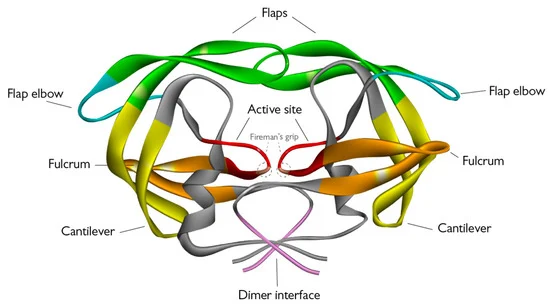
\includegraphics[width=\textwidth]{/Users/enrico/PROTEINS/tesi/immagini_tesi_ingelse/viruses-15-00712-g003-550.png}
    \caption{Structure of HIV Protease.}
    \label{fig:HIV}
\end{figure}



\newpage


\section{PDZ Domain and 3LNX}
\noindent  In molecular biology, a domain is a specific region of a protein that can perform a structural or functional role independently from the rest of the protein.\cite{ref8} \\
They are tipycally characterized by two main characteristics; the first it is that the domain (as we said a portion of the protein) can fold into a three-dimensional structure on its own, the second is that it can play an indipendent role when it is unit with a protein.
In addition, because it is a modular unit, it is used by other proteins to form more complex structures.\cite{ref8} \\
Proteins often consist of multiple domains arranged in various combinations, creating multifunctional macromolecules capable of complex interactions. 

The PDZ domain is a well-studied example of a protein domain.\\
It is named after the three proteins in which it was first identified (Postsynaptic density protein 95,Drosophila discs large protein, Zona Occludens), it is a modular domain, its function is to organize and stabilize large multiprotein complexes, maintaining cellular architecture and facilitating biochemical signaling pathways. \cite{ref8}\\
The PDZ domain typically consists of 80--90 amino acid; facilitates protein-protein interactions by recognizing specific peptide sequences, often located at the C-terminal region of target proteins; assemble protein complexes at cellular membranes
In this work we will see the 3LNX protein, which is a PDZ-specific domain.\\
The 3LNX protein offers important insights into the functioning of these domains.\\
This protein has a hydrophobic pocket that accommodates a external peptide, that binds with the 3LNX.\\
It is constitute from three alpha helix, that we will call alpha-$\alpha$, alpha-$\beta$ and $alpha-\gamma$, and six different beta-sheet, that we will call beta-$\alpha$, beta-$\beta$, $beta-\gamma$,$beta-\delta$, $beta-\epsilon$,$beta-\eta$. \\
\begin{figure}[H]
    \centering
    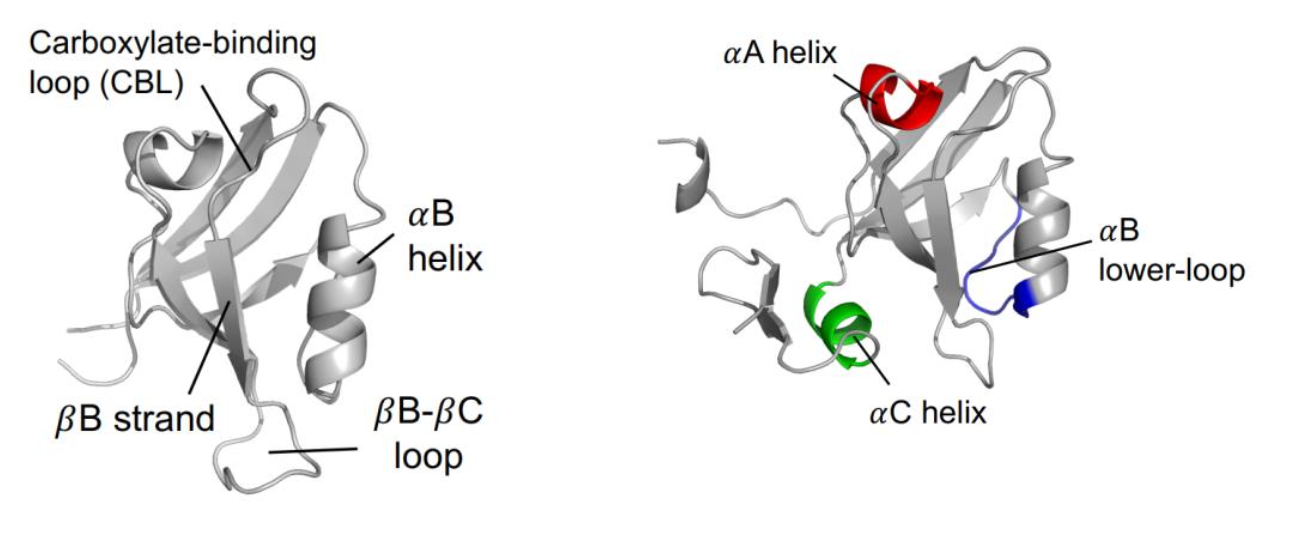
\includegraphics[width=1\textwidth]{/Users/enrico/PROTEINS/tesi/immagini_tesi_ingelse/Screenshot 2024-12-17 at 08.59.09.png}
    \caption{3LNX protein}
\end{figure}
The allosteric mechanism works as follows: a perturbation at one allosteric site propagates a signal towards the hydrophobic pocket, located between the $\beta$-sheet and the $\alpha$-helix. \\
This pocket can transition between open and closed states, which is the essence of allostery, preventing a ligand from binding or unbinding at the active site within the hydrophobic pocket. \\
These allosteric sites do not directly interact with the ligand but are crucial for transmitting structural changes within the protein upon ligand binding. In this study, we will investigate in detail two potential allosteric sites, identified by experimental biologists, located in the $\alpha$-helix and the $\gamma$-helix, as suggested by previous research. \cite{ref15}.\\
So this is the schema of what we expect:


\begin{tikzpicture}[node distance=2cm]

    % Nodes for perturbation and regions
    \node (alphaalpha) [draw, rectangle, text centered, minimum height=1cm, minimum width=2cm] {alpha-$\alpha$ helix};
    \node (alphabeta) [draw, rectangle, text centered, minimum height=1cm, minimum width=2cm, right=of alphaalpha] {alpha-$\gamma$ helix};
    
    % Nodes for regions below alpha-alpha and alpha-gamma, aligned horizontally
    \node (bindingAlphaAlpha) [below of=alphaalpha, draw, rectangle, text centered, minimum height=1cm, minimum width=2.5cm, yshift=-1cm] {Binding Pocket};
    \node (bindingAlphaGamma) [below of=alphabeta, draw, rectangle, text centered, minimum height=1cm, minimum width=2.5cm, yshift=-1cm] {Binding Pocket};
    
    % Draw arrows from alpha-alpha and alpha-gamma to each region
    \draw[->] (alphaalpha) -- (bindingAlphaAlpha);
    \draw[->] (alphabeta) -- (bindingAlphaGamma);

\end{tikzpicture}







\newpage
\chapter{Normal and functional mode Analysis}
\section{Introduction}
\noindent We aim to study how the atoms comprising a protein oscillate around their equilibrium positions, thereby propagating signals and interacting with one another.\\
For this investigation, we utilize Normal Mode Analysis (NMA).\\
It is a technique that delineates a system in terms of its normal modes.\\
These modes provide a quantitative method to evaluate the vibration intensity of each atom in the system.\\
Arising from a harmonic (Gaussian) approximation, the normal modes can be collective movements at either low or high frequencies.\\
This technique precisely describes the vibrations of atoms at their equilibrium points. Using this method, we can identify the modes and the most critical sites for allosteric mechanisms.\\
Thus, NMA establishes a connection between structure, function, and dynamics; indeed, by starting with the geometric structure of the protein, we can compute the normal modes and employ them to examine allostery in proteins.
Hence, NMA serves as a theoretical bridge linking the structure and function of a protein.



\section{Gaussian Network Model and Normal Mode Analysis}
\noindent For studying the oscillation of the atoms around their equilibrium position we need to start defining the Hamiltonian of the system.\\
If the protein is at equilibrium, we expect that the Hamiltonian is a function of a potential that depends on the position of every atom constituting the PDZ-specific domain and on bonding forces between atoms, electrostatic and Van der Waals interactions, solvent forces, and many additional factors.\\
As it clear, it is very complex to develop a real world model in this field, 
however, this is not our goal.\\
In fact our aim is to understand how much of the allosteric mechanism in proteins is explainable only from its geometric factor.\\
Thus we represent the Hamiltonian of the system as H=V(r) where r is the vector containing the positions of all the atoms that make up the protein, so it depends only from this positions and not from other factors.\\
So we bet on the assumption that the protein’s dynamics can be effectively described using only its geometric structure, 
specifically focusing on the positions of the backbone atoms (alpha-carbons), 
while neglecting finer details such as side-chain interactions or solvent effects.\\
In fact we believe that years of evolutionary optimization have led to a protein structure that is highly efficient and optimized for its function.\\
While this simplification allows for manageable computational complexity, it may overlook important local and long-range interactions.\\
Also in this way due to the complexity of the system, it is not feasible to solve it exactly.\\
Therefore, we rely on approximations, such as the second-order expansion of the potential energy around an equilibrium point, 
which provides a simplified representation of the protein's behavior.\\
However, this approximation neglects higher-order interactions that could influence the protein’s dynamics, and as a result, it may fail to capture certain intricate behaviors, especially in regions where the protein undergoes significant conformational changes.\\
Mathamically the second-order approximation of a function \( V({r}) \), around an equilibrium point \( {r}_0 \), can be expressed as:\cite{ref9}

\begin{equation}
V({r}) \approx V({r}_0) + \nabla V({r}_0)^\top ({r} - {r}_0) + \frac{1}{2} ({r} - {r}_0)^\top {H_V} ({r} - {r}_0),\label{hessian}
\end{equation}


where:
\begin{itemize}
    \item \( V({r}_0) \) is the value of the function at the equilibrium point \( {r}_0 \).
    \item \( \nabla V({r}_0) \) is the gradient of the function, defined as:
    \begin{equation}
    \nabla V({r}) = \frac{\partial V}{\partial {r}} \bigg|_{{r} = {r}_0},
    \end{equation}
    which equals zero if \( {r}_0 \) represents a minimum point, corresponding to the equilibrium position.
    \item \( {H_V} \) is the Hessian matrix of \( V({x}) \), defined as:
    \begin{equation}
    {H_V} = \frac{\partial^2 V}{\partial {r}^2} \bigg|_{{x} = {x}_0}=\[
        \begin{bmatrix}
        \frac{\partial^2 V}{\partial x_1^2} & \frac{\partial^2 V}{\partial x_1 \partial x_2} & \cdots & \frac{\partial^2 V}{\partial x_1 \partial x_{3N}} \\
        \frac{\partial^2 V}{\partial x_2 \partial x_1} & \frac{\partial^2 V}{\partial x_2^2} & \cdots & \frac{\partial^2 V}{\partial x_2 \partial x_{3N}} \\
        \vdots & \vdots & \ddots & \vdots \\
        \frac{\partial^2 V}{\partial x_{3N} \partial x_1} & \frac{\partial^2 V}{\partial x_{3N} \partial x_2} & \cdots & \frac{\partial^2 V}{\partial x_{3N}^2}
        \end{bmatrix}.
    \]
    \end{equation}
    This matrix format ensures that all interactions between positional variables are considered for each pair of dimensions, crucial for accurately modeling the dynamics and for the normal modes.
\end{itemize}








Because working in high dimensions is complex, we will also introduce an isotropic approximation of the system (In the following lines, we will examine the drawbacks.). However, the system can be easily generalized to the anisotropic case as well.\\
Now we have a gaussian model which is a springs model, where every atom is connected with the other atoms with a spring.\\
If we want that only some residues are connected we can put a cutoff distance, so that the spring is connected only with the atoms that are in a certain distance.\\
In this way hamiltonian become:
\begin{equation}
    H({x}) = \frac{g}{2} \sum_{i,j} x_i K_{ij} x_j.
\end{equation}
Where \( K \) is the Kirchhoff matrix which is the Hessian matrix of the system and \( g \) is a adjustable energy scale that can be set by matching the theoretical mean square displacement of the displacement from their native positions.\\
The Kirchhoff matrix is a matrix that represents the connections between nodes in a graph, without encoding information about its physical layout.\\
For a graph \( G \) with \( n \) vertices, the Kirchhoff matrix \( K \) is defined as:\cite{ref11}
\begin{equation}
    K = D - A \label{Kirchhoff}
\end{equation}
Where \( D \) is the degree matrix, a diagonal matrix defined as:
\begin{equation}
    D_{ij} = 
    \begin{cases} 
      \deg(v_i) & \text{if \( i = j \),} \\
      0 & \text{if \( i \neq j \),}
    \end{cases}
\end{equation}
where \( \deg(v_i) \) is the degree of vertex \( v_i \), the number of edges connected to vertex (nodes) \( i \); and \( A \) is the adjacency matrix, a square matrix defined as:
\begin{equation}
    A_{ij} = 
    \begin{cases} 
      1 & \text{if there is an edge between vertices } v_i \text{ and } v_j, \\
      0 & \text{otherwise}.
    \end{cases}
\end{equation}

By the symmetry property of \( K \), it follows that it is diagonalizable, it is positive semi-definite, and its smallest eigenvalue is always 0.
Because it is positive semi-definite, \( K \) does not have a conventional inverse, but we can obtain the pseudo-inverse which is the matrix \( K^+ \) that minimizes the following equation: 
\[
K^+ K = K K^+ = I - \frac{1}{n} \mathbf{1} \mathbf{1}^\top
\]
where \( n \) is the number of nodes and \( \mathbf{1} \) is a vector of all ones.

\begin{figure}[h]
    \centering
    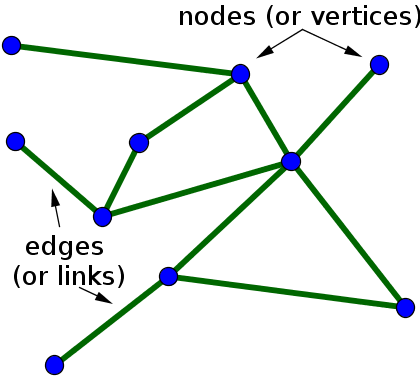
\includegraphics[width=0.5\textwidth]{/Users/enrico/PROTEINS/tesi/immagini_tesi_ingelse/small_undirected_network_labeled-2.png}
    \caption{Schematic representation of a Network.}
    \label{fig:Network}
\end{figure}




This modeling is called Gaussian Network Model (GNM) and is commonly used to study the dynamic of proteins.\\
So to summarize this is a model which take in consideration only the geometric structure of the protein and no one of the other type of interactions. \\
In fact the GNM assumes that interactions between atoms in a protein can effectively be represented as elastic springs with uniform force constants. 
This linearity assumption implies that any deviation from equilibrium can be treated as a small, 
reversible perturbation that does not substantially alter the basic structure of the protein.\\
In addition it ignores the solvent effects and he model does not distinguish between different types of bonds, 
such as hydrogen bonds, van der Waals interactions, or electrostatic interactions, 
treating all interactions as if they had the same impact on protein dynamics.\\
Moreover, the GNM inherently assumes isotropy in the protein's interaction network, treating the protein structure as if it uniformly responds to perturbations in any direction. This isotropic assumption simplifies the mathematical treatment of protein dynamics by not requiring differential responses based on directional changes. While this makes the model computationally efficient, it overlooks the potential anisotropy in biological molecules, where directional dependencies are crucial for functions such as enzyme binding, signal transduction, and structural stability.\\
This isotropy assumption is reflected in the uniform force constants across all interactions, irrespective of their nature or directional orientation, further abstracting the model from the nuanced, directionally dependent behaviors seen in real protein dynamics. Such simplifications, while useful for broad analyses, might not capture critical aspects of protein functionality that depend on highly directional, anisotropic interactions. Therefore, while the GNM offers significant insights into protein behavior under the assumption of isotropic interactions, it might miss critical dynamics relevant in physiological conditions where anisotropy plays a key role.\\

Now for solving this system we need the normal modes, which are the eigeinvectors of the kirchoff matrix.
\begin{equation}
    {K} {v}_k = \lambda_k {v}_k. \label{equazione}
\end{equation}
In addition this modes are very usefull because they allow us to interpretate the motion of the atoms in the protein.\\
In fact now we can solve our motion's equation:
\begin{equation}
{F} = -\nabla V({x}) = -{K} {x} = {M} \ddot{{x}}.
\end{equation}
where \( {M} \) is the diagonal mass matrix.\\
Now we normalize the coordinates with a change of variable: \( {x}' = \sqrt{M} {x}\). \\
So substituting this transformation we obtain:
\begin{equation}
\ddot{{x}} = -{K} {x}.
\end{equation}
The solution of this equation is of the form \( {x}(t) = {v}_k e^{i \omega_k t} \), where \( \omega_k \) is the angular frequency of the \( k \)-th mode and \( {v}_k \) is the corresponding eigenvector.\\
Substituting this into the equation of motion:

\begin{equation}
-\omega^2 {v}_k = -{K} {v}_k.
\end{equation}
Mathematically normal modes are the eigenvectors \( {v}_k \) of the Hessian matrix and we use them to solve the system. 
This equation demonstrates that \( \lambda_k \), the k-th eigenvalue of the Hessian, is related to the angular frequency by, as equation \ref{equazione}:
\begin{equation}
    \omega_k = \sqrt{\lambda_k}.
\end{equation}

The interpretation of that is that the eigenvectors \( {v}_k \) tell us the directions of motion in the space of atomic coordinates and every mode represent a distinct oscillation of every atoms of the protein.\\
In addition the low intensity values of eigenvalues correspond to low frequency modes are usually in literature associate with long range effect and high frequency oscillationa re associated with local effects.
Typically the long range modes are assocaited with functions like the opening and closing of ligand-binding sites which are  allosteric transitions, 
We will use them to solve the system as we see in a few lines.\\

Now from the hamiltonian and from the normal modes we can compute two important quantities that are the probability density and the mean displacement between the atoms.\\
From this simple hamiltonian formulation of the system we can derive some statistical properties.
The probability density at equilibrium is given by:\cite{ref12}
\begin{equation}
    P({x}) = \frac{1}{Z} e^{-\beta H({x})},
\end{equation}
where the partition function \(Z\) is:
\begin{equation}
    Z = \int e^{-\beta H({x})} \, d{x}.
\end{equation}

Define it we can use it to compute a lot of important quantities, like for exemple the mean displacement of the atoms.\\
The mean position \(\langle {x} \rangle\) can be calculated as:\cite{ref12}
\begin{equation}
    \langle {x} \rangle = \int {x} P({x}) \, d{x},
\end{equation}
where:
\begin{equation}
    P({x}) = \frac{1}{Z} e^{-\frac{\beta}{2} {x}^\top {g}{K} {x}},
\end{equation}
and the partition function is:\cite{ref12}
\begin{equation}
    Z = \int e^{-\frac{\beta}{2} {x}^\top {g}{K} {x}} \, d{x}.
\end{equation}

Substituting \(P({x})\) into the expression for \(\langle {x} \rangle\), we obtain:
\begin{equation}
    \langle {x} \rangle = \frac{1}{Z} \int {x} e^{-\frac{\beta}{2} {x}^\top {g}{K} {x}} \, d{x}.
\end{equation}

Since the integrand \({x} e^{-\frac{\beta}{2} {x}^\top {g}{K} {x}}\) is symmetric with respect to \({x}\), and there are no linear terms in the Hamiltonian, the Gaussian distribution is centered at \({x} = 0\). Therefore:\cite{ref12}
\begin{equation}
    \langle {x} \rangle = 0.
\end{equation}

\newpage
\section{Stochastic Processes} \label{sec:stochastic_processes}

\noindent We use a stochastic process to model the oscillation around the equilibrium position of each atom that constitutes the protein.\\

To model the oscillation, we use the following equation:
\[
m \frac{d^2\mathbf{x}}{dt^2} = -\gamma \frac{d\mathbf{x}}{dt} - \nabla H(\mathbf{x}) + \sqrt{2 \gamma k_B T} \, \boldsymbol{\eta}(t) = -\gamma \frac{d\mathbf{x}}{dt} - g \mathbf{K} \mathbf{x} + \sqrt{2 \gamma k_B T} \, \boldsymbol{\eta}(t),
\]
where (\mathbf{x}(t)\) is a vector representing the displacement of residues from their equilibrium positions; \(H(\mathbf{x})\) is a scalar function (the Hamiltonian); \(\boldsymbol{\eta}(t)\) is a vector of Gaussian white noise with zero mean and unit variance; \(m\) and \(\gamma\) are scalars representing the mass and the damping coefficient, respectively; 
\(\mathbf{K}\) is a matrix of coupling constants between residues (symmetric and positive definite) and \(g\) is a scalar that normalizes \(\mathbf{K}\).\\
In the overdamped regime (\(\gamma \gg m\)), the acceleration term can be neglected, simplifying the equation to:
\[
\gamma \frac{d\mathbf{x}}{dt} = - g \mathbf{K} \mathbf{x} + \sqrt{2 \gamma k_B T} \, \boldsymbol{\eta}(t).
\]
To further simplify the equation, we introduce a new time scale:
\[
\tau = \frac{t}{\gamma}, \quad dt = \gamma d\tau,
\]
and normalize the Hamiltonian by working in units of \(H_0 = 2 k_B T\):
\[
\tilde{H}(\mathbf{x}) = \frac{H(\mathbf{x})}{H_0}.
\]
The equation then becomes:
\[
\frac{d\mathbf{x}}{d\tau} = -\nabla \tilde{H}(\mathbf{x}) + {\boldsymbol{\eta}}(\tau) = -g \mathbf{K} \mathbf{x}(t) + \boldsymbol{\eta}(t),.
\]


This dynamics corresponds to a multidimensional Ornstein-Uhlenbeck process, the simplest Gaussian process with mean-reverting properties.\\

The matrix \(\mathbf{K}\) can be diagonalized:
\[
\mathbf{K} = \mathbf{V} \boldsymbol{\Lambda} \mathbf{V}^\dagger,
\]
where \(\mathbf{V}\) is the orthogonal matrix of eigenvectors (\(\mathbf{V}^\dagger = \mathbf{V}^{-1}\)) of \(\mathbf{K}\) 
and \(\boldsymbol{\Lambda} = \text{diag}(\lambda_1, \lambda_2, \dots, \lambda_N)\) is the diagonal matrix of eigenvalues of \(\mathbf{K}\).\\
Changing variables to the eigenbasis:
\[
\tilde{\mathbf{x}}(t) = \mathbf{V}^\dagger \mathbf{x}(t),
\]
the equation becomes:
\[
\frac{d \tilde{\mathbf{x}}(t)}{dt} = - g \boldsymbol{\Lambda} \tilde{\mathbf{x}}(t) + \tilde{\boldsymbol{\eta}}(t),
\]
where \(\tilde{\boldsymbol{\eta}}(t) = \mathbf{V}^\dagger \boldsymbol{\eta}(t)\). Since the transformation is orthogonal, \(\tilde{\boldsymbol{\eta}}(t)\) remains Gaussian white noise with the same properties as \(\boldsymbol{\eta}(t)\).
The diagonalization decouples the sysssstem into independent equations for each mode \(k\):
\[
\frac{d \tilde{x}_k(t)}{dt} = -g \lambda_k \tilde{x}_k(t) + \tilde{\eta}_k(t),
\]
where \(\tilde{x}_k(t)\) is the \(k\)-th component of \(\tilde{\mathbf{x}}(t)\),
\(\lambda_k\) is the \(k\)-th eigenvalue of \(\mathbf{K}\),
and \(\tilde{\eta}_k(t)\) is the \(k\)-th component of the transformed noise.
The solution to the Ornstein-Uhlenbeck equation for each mode is:
\[
\tilde{x}_k(t) = \tilde{x}_k(0) e^{-g \lambda_k t} + \int_0^t e^{-g \lambda_k (t-s)} \tilde{\eta}_k(s) \, ds.
\]
This solution reveals the direction in the eigenvector space of residue fluctuation. The corresponding eigenvalue is proportional to the intensity of its oscillation, which is useful for understanding the role of each residue in the context of collective behavior.
We will use this solution heavily in the following sections to analyze the allosteric propagation of signals in the protein.\\









\newpage











































\newpage
\chapter{Introduction to causality and causality in allosteric mechanisms of proteins}
\noindent Our primary aim, as we just said, is to identify  the allosteric propagation of the signal from allosteric sites to other sites of the protein.\\
Generally causality refers to the relationship between causes and effects, where one event (the cause) directly influences or produces another event (the effect), so it implies a directional influence.\\
To understand the propagation of the signal we need to have a cause (the sorgent of the signal, in our case the allosteric site) and an effect (the dynamical changing in the protein).\\
To reveal causality we saw, for now, only one useful indicator: the covariance.\\
But we know that Covariance does not imply causation, so in the following pages we will discover new causal indicators.\\
While covariance is a starting point for identifying potential causal relationships, it primarily measures the strength of linear associations without providing directionality or confirming causation.\\
This limitation necessitates the introduction of more sophisticated indicators that can discern direct from indirect influences and clarify the pathways through which allosteric signals propagate.\\
To overcome the limitations of covariance, we will introduce additional causal indicators such as response functions and transfer entropy. \\
These indicators provide a more nuanced understanding of the causal relationships within proteins, allowing us to identify the specific residues and regions that play a crucial role in allosteric mechanisms.\\
Infact they are able to measure the casual relation in a different way from the covariance, in fact the response allows us to understand the direct relationship between residues and trasnfer entropy to catch the non linear interactions and so the directioanal flux of information. \\
These indicators not only measure the strength of associations but also help determine the direction and specificity of interactions, crucial for mapping the complex networks within proteins.

\begin{figure}[h]
    \centering
    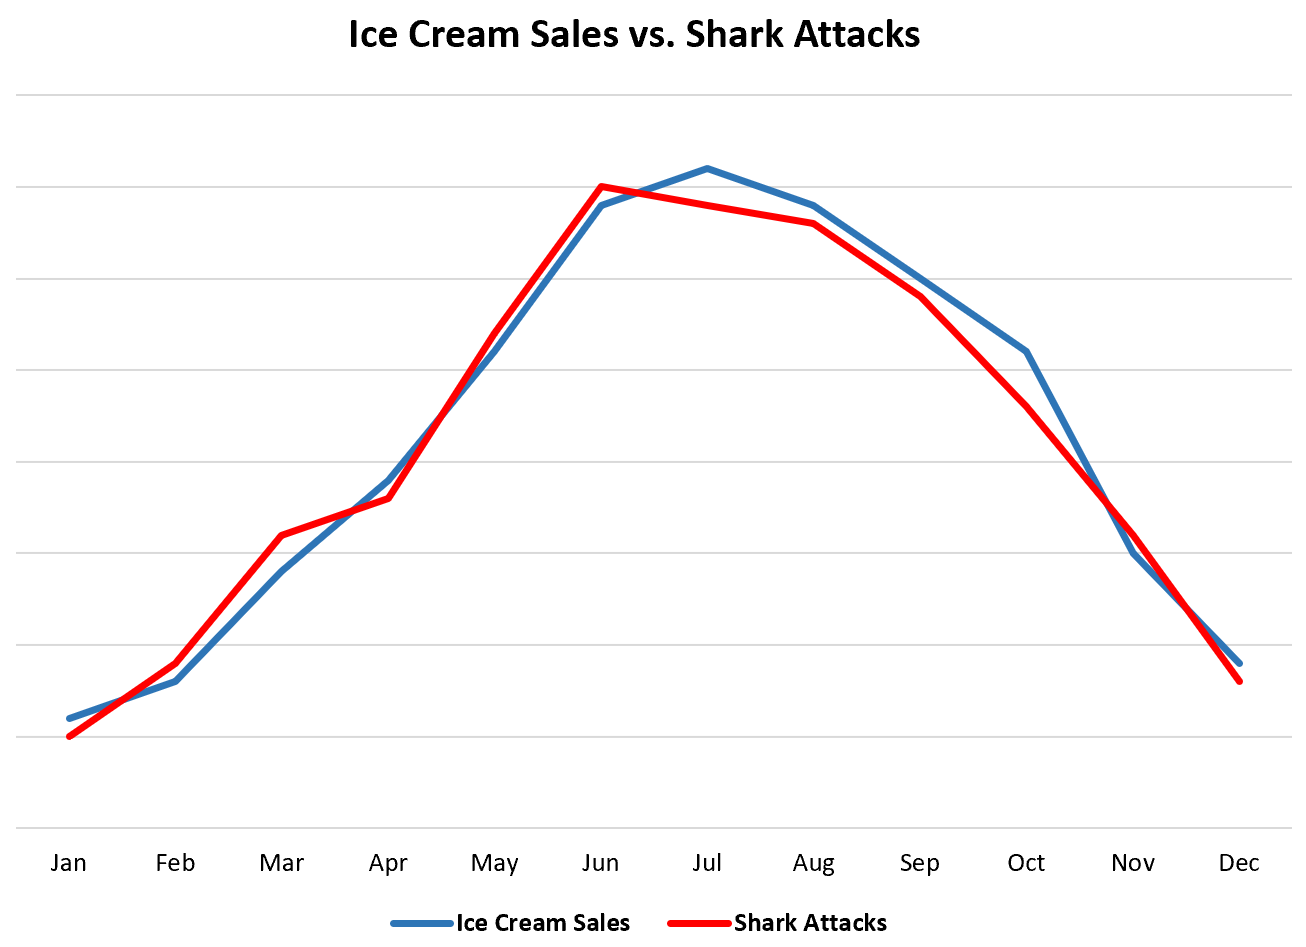
\includegraphics[width=\textwidth]{/Users/enrico/PROTEINS/tesi/immagini_tesi_ingelse/corrCause1.png}    
    \caption{Covariance is not causation. The Covariance between two variables does not imply a causal relationship. This is an exemple of a spurious Covariance. Here the latent variable is the temperature.}
    \label{fig:Covariance is not causation}
\end{figure}
\newpage
Mathematically causal relationships are often modeled as:\cite{ref14}
\[
B = f(A, \text{other factors}),
\]
where \( f \) describes how \( A \) and other factors jointly determine \( B \).\\
It is hard to understand causality in the real world, particularly in biological systems where the interactions between components are numerous and there are many factors that can influence the system. \\
Thus, testing if there is a causal relationship between two variables is a very challenging task, because my function depends on many other variables, making it difficult to discern whether changes in the output are related to changes in my specific variable or due to other changes. \\
Causality is very important because it allows us to understand which variables and dimensions are crucial for my system to infer a specific output. In a data-driven system for inferring causality, if we add many dimensions hoping to find patterns or covariance to predict the output, we encounter the problem of the curse of dimensionality, and thus our model will likely fail in its forecasting. \\
Therefore, understanding causality is very important for the inference of the system because it not only helps to better understand the phenomenon but also to build more effective inference models. \\
Today, there is no unique method to infer causality; instead, there are many methods that can be used for inference. \\
Each of these methods has its own advantages and disadvantages, but we cannot be certain that we have established true causality. \\
In our case, we are also dealing with a high-dimensional system, where moving a single residue results in collective motion along the protein, with various sections of the protein responding in very different ways.\\

Causality (and one of causal indicator which we will use) is connect to the concept of entropy and Shannon entropy.\\
Typically if we are forecasting a output X variable we can define a Shannon entropy associated with that output, defined as:
\[
H(X) = -\sum_{i} P(x_i) \log P(x_i),
\]
where \( X \) is a discrete random variable with possible states \( x_i \), and \( P(x_i) \) is the probability of \( x_i \).\\
When \( P(x_i) = \delta(x_i) \) -> \( H(X) = 0 \), the system has no uncertainty, indicating complete predictability.\\
So if my target variable has the distribution of the delta function, the entropy is zero, so the system is deterministic.\\
So the distribution width of the \( x_i \) determines how much my system is predictable.
In general more the entropy is low, more the system is predictable, so more we know causal relation of the system.\\
The discussion on causality will be expanded to connect theoretical concepts with biological implications more directly.\\
This will include illustrations of how changes at an allosteric site can causally influence the active site's functionality, using specific biochemical pathways as examples.\\
This approach will help bridge the gap between abstract statistical measures and their tangible effects on protein behavior.\\
Now we will see some indicators to try to catch the allosteric causality mechanism in the system.\\
To further ground our discussion in practical terms, we will explore how allosteric mechanisms, often triggered by external stimuli or internal chemical changes, lead to observable changes in protein activity. This exploration will serve as a foundation to understand how subtle molecular changes can result in significant biological outcomes, emphasizing the importance of pinpointing the origin of these signals.


\newpage
\section{Covariance}
\noindent
The Covariance between two variables, such as the fluctuations in the positions of residues \( i \) and \( j \), provides insight into how these components of the system interact.\\
The covariance of the displacement \({x}(t)\) is defined as:\cite{ref13}
\[
{C}(t) = \langle {x}(t) {x}^\top(0) \rangle,
\]
where \({x}(t) = {V} \tilde{{x}}(t)\). Substituting this into the definition:
\[
{C}(t) = {V} \langle \tilde{{x}}(t) \tilde{{x}}^\top(0) \rangle {V}^\top.
\]
Substituting the solution of $\tilde{{x}}$ into the covariance:
\[
\langle \tilde{{x}}(t) \tilde{{x}}^\top(0) \rangle = \langle \tilde{{x}}(0) e^{-{g \Lambda} t} \tilde{{x}}^\top(0) \rangle + \left\langle \left( \int_0^t e^{-g {\Lambda} (t-s)} \tilde{{\eta}}(s) \, ds \right) \tilde{{x}}^\top(0) \right\rangle.
\]
For the first term:
\[
\langle \tilde{{x}}(0) e^{-{g \Lambda} t} \tilde{{x}}^\top(0) \rangle = e^{-{g \Lambda} t} \langle \tilde{{x}}(0) \tilde{{x}}^\top(0) \rangle.
\]
In the stationary regime:
\[
\langle \tilde{x}_k(0) \tilde{x}_l(0) \rangle =  \frac{\delta_{kl}}{g \lambda_k}.
\]
Thus:
\[
\langle \tilde{{x}}(0) \tilde{{x}}^\top(0) \rangle = ({g \Lambda})^{-1}.
\]
Substitute this:
\[
\langle \tilde{{x}}(0) e^{-{g \Lambda} t} \tilde{{x}}^\top(0) \rangle = e^{-{g \Lambda} t} \cdot ({g \Lambda})^{-1} .
\]
For the second term:
\[
\left\langle \left( \int_0^t e^{- g {\Lambda} (t-s)} \tilde{{\eta}}(s) \, ds \right) \tilde{{x}}^\top(0) \right\rangle = 0,
\]
because \(\tilde{{\eta}}(s)\) is uncorrelated with \(\tilde{{x}}(0)\).
Thus, the stochastic contribution vanishes.\\
The covariance in the eigenbasis is:
\[
\langle \tilde{{x}}(t) \tilde{{x}}^\top(0) \rangle = e^{-{g \Lambda} t} \cdot ({g \Lambda})^{-1}.
\]
Transform back to the original basis:
\[
{C}(t) = {V} \langle \tilde{{x}}(t) \tilde{{x}}^\top(0) \rangle {V}^\top.
\]

Substitute the eigenbasis covariance:
\[
{C}(t) = {V} \left( e^{-{g \Lambda} t} \cdot ({g \Lambda})^{-1}  \right) {V}^\top.
\]


Or in components:
\[
C_{ij}(t) = \sum_{k=1}^N v_{ik} v_{jk} \frac{e^{-g \lambda_k t}}{g \lambda_k} ,
\]

Positive Covariances between residues \(i\) and \(j\) at time \(t\) indicate that the fluctuations in their positions are synchronized, while negative Covariances suggest that the fluctuations are anti-correlated.\\
Both positive and negative Covariances can reveal how residues interact and influence each other's dynamics.\\
As we just said it reveals a possible causal relationship between the residues, in addition we need a storng Covariance to find causality, but it is not sufficient condition to have causality.\\
\newpage



\section{Response Function}
\noindent Another indicator of causality is the linear response function, which quantifies the influence of a perturbation on one residue on the behavior of another residue.\\
The response function \(R_{ij}(t)\) is defined as:\cite{ref13}
\begin{equation}
    R_{ij}(t) = {C_{ij}(t)}{C^{-1}_{ij}(0)},
\end{equation}

Where \(C_{ij}(t)\) is the covariance between residues \(i\) and \(j\) at time \(t\).\\
So it is completely determined by the covariance.\\
Substituting it we obtain:
\[
R_{ij}(t) = \frac{1}{N}+{\sum_{k=1}^N  v_{ik} v_{kj} e^{-g \lambda_k t}}.
\]
The linear response describes how the average position of a residue $i$, denoted as $\langle {x}_i \rangle$, responds to a perturbation applied to another residue $j$ through an external force $f_j$. 
The power of this indicator is that it tends to ignore the spurious Covariance beacuse it ignores the non direct interaction between the residues.\\
To let see why there is a perturbation and why it is connected with the covariance we need to see the fluctuation-dissipation theorem.\\
Infact if we consider the Hamiltonian of the system under a small external perturbation:
\begin{equation}
    \mathcal{H} = \mathcal{H}_0 - \sum_j f_j {x}_j,
\end{equation}
where $\mathcal{H}_0$ is the unperturbed Hamiltonian and $-f_j {x}_j$ is the interaction term between the external force and the displacements of residues $j$;
we obtain that average position of dispalcement of residue $i$ is:
\begin{equation}
\langle {x}_i \rangle = \frac{\int {x}_i e^{-\beta \mathcal{H}} \, d{x}}{\int e^{-\beta \mathcal{H}} \, d{x}}.
\end{equation}
Expanding the exponential $e^{-\beta \mathcal{H}}$ to first order in the perturbation $f_j$:
\begin{equation}
e^{-\beta \mathcal{H}} \approx e^{-\beta \mathcal{H}_0} \left( 1 + \beta f_j {x}_j \right),
\end{equation}
and substituting this expansion into the expression for $\langle {x}_i \rangle$:
\begin{equation}
\langle {x}_i \rangle \approx \langle {x}_i \rangle_0 + \beta f_j \langle \delta {x}_i \cdot \delta {x}_j \rangle,
\end{equation}
Taking the derivative of $\langle {x}_i \rangle$ with respect to $f_j$ gives the linear response:
\begin{equation}
R_{ij} = \frac{\partial \langle {x}_i \rangle}{\partial f_j} = \beta \langle \delta {x}_i \cdot \delta {x}_j \rangle. \label{response}
\end{equation}
This result shows that the response $R_{ij}$ is directly proportional to the equilibrium covariance between the fluctuations of the displacement of residue $i$ and $j$.\\

\newpage
\section{Transfer Entropy}
\noindent The last causal indicator is the Transfer Entropy (TE), which quantifies the directional flow of information between two variables.\\
It add to the previous indicator the non linearity and directional information, so it is very useful to understand the causal relationship between the residues.\\
It quantifies how much the knowledge of past states of \(x_j\) improves the prediction of future states of \(x_i\), beyond what is already provided by the past states of \(x_i\) itself. \\
The TE is defined as:\cite{ref13}
\[
TE_{j \to i}(t) = H[x_i(t + \tau) \mid x_i(\tau)] - H[x_i(t + \tau) \mid x_i(\tau), x_j(\tau)]
\]
where \(H[a \mid b]\) is the conditional Shannon entropy of variable \(a\) given \(b\), \(x_i(t + \tau)\): 
State of \(x_i\) at time \(t + \tau\), \(x_i(\tau), x_j(\tau)\) are the state of \(x_i\) and \(x_j\) at time \(\tau\).\\

For stationary Gaussian processes, TE can be computed analytically using the covariance matrices of the processes involved. \\
The TE from \(x_j\) to \(x_i\) at a time lag \(t\) is given by:\cite{ref13}
\begin{equation}
TE_{j \to i}(t) = -\frac{1}{2} \ln{1 - \frac{\alpha_{ij}(t)}{\beta_{ij}(t)}}=TE_{i,j},\label{TE}
\end{equation}
where:
\begin{equation}
\alpha_{ij}(t) = \left[C_{ii}(0)C_{ij}(t) - C_{ij}(0)C_{ii}(t)\right]^2,\label{alpha}
\end{equation}
\begin{equation}
\beta_{ij}(t) = \left[C_{ii}(0)C_{jj}(0) - C_{ij}^2(0)\right]\left[C_{ii}^2(0) - C_{ii}^2(t)\right].\label{beta}
\end{equation}
So also it is completely determined by the covariance.\\
The derivation of Transfer Entropy (TE) for Gaussian systems leverages the fact that the entropy of a multivariate Gaussian distribution depends only on the determinant of its covariance matrix.\\
This section provides a step-by-step explanation of the derivation for \( TE_{j \to i}(t) \).\cite{ref13}
Consider a system described by the variables \(x_i(t)\), \(x_i(0)\), and \(x_j(0)\). The joint covariance matrix of these variables is:
\[
\Omega = \begin{bmatrix}
C_{ii}(0) & C_{ii}(t) & C_{ij}(t) \\
C_{ii}(t) & C_{ii}(0) & C_{ij}(0) \\
C_{ij}(t) & C_{ij}(0) & C_{jj}(0)
\end{bmatrix},
\]
where \(C_{ii}(0)\) and \(C_{jj}(0)\) are the variances of \(x_i\) and \(x_j\), respectively, \(C_{ii}(t)\) is the autocovariance of \(x_i\) at time lag \(t\), \(C_{ij}(t)\) is the cross-covariance between \(x_i(t)\) and \(x_j(0)\), \(C_{ij}(0)\) is the instantaneous cross-covariance between \(x_i(0)\) and \(x_j(0)\).\\
The entropy of a multivariate Gaussian distribution is given by:
\[
H({x}) = \frac{1}{2} \ln{[(2\pi e)^n \det(\Sigma)]},
\]
where \(n\) is the dimensionality of \({x}\), and \(\Sigma\) is its covariance matrix.\\
For the variables \([x_i(t), x_i(0), x_j(0)]\), the entropy is:
\[
H(x_i(t), x_i(0), x_j(0)) = \frac{1}{2} \ln{[(2\pi e)^3 \det(\Omega)]}.
\]
The conditional entropy of \(x_i(t)\) given \([x_i(0), x_j(0)]\) is computed using the Schur complement.\\
For a covariance matrix partitioned as:
\[
\Omega = \begin{bmatrix}
A & B \\
B^\top & C
\end{bmatrix},
\]
the Schur complement of \(C\) in \(\Omega\) is:
\[
\Sigma_{x_i(t) | x_i(0), x_j(0)} = A - B C^{-1} B^\top.
\]

In our case, the conditional covariance matrix for \(x_i(t)\) given \(x_i(0)\) and \(x_j(0)\) is:
\[
\Sigma_{x_i(t) | x_i(0), x_j(0)} = C_{ii}(0) - \begin{bmatrix}
C_{ii}(t) & C_{ij}(t)
\end{bmatrix}
\begin{bmatrix}
C_{ii}(0) & C_{ij}(0) \\
C_{ij}(0) & C_{jj}(0)
\end{bmatrix}^{-1}
\begin{bmatrix}
C_{ii}(t) \\
C_{ij}(t)
\end{bmatrix}.
\]

The entropy is then:
\[
H(x_i(t) | x_i(0), x_j(0)) = \frac{1}{2} \ln{[2\pi e \det\left(\Sigma_{x_i(t) | x_i(0), x_j(0)}\right)]}.
\]

Similarly, the conditional covariance matrix for \(x_i(t)\) given \(x_i(0)\) is:
\[
\Sigma_{x_i(t) | x_i(0)} = C_{ii}(0) - \frac{C_{ii}^2(t)}{C_{ii}(0)}.
\]

The entropy is:
\[
H(x_i(t) | x_i(0)) = \frac{1}{2} \ln{[2\pi e \det\left(\Sigma_{x_i(t) | x_i(0)}\right)]}.
\]


Transfer Entropy is defined as:
\[
TE_{j \to i}(t) = H(x_i(t) | x_i(0)) - H(x_i(t) | x_i(0), x_j(0)).
\]

Substituting the expressions for the conditional entropies:
\[
TE_{j \to i}(t) = \frac{1}{2} \ln{[\frac{\det{(\Sigma_{x_i(t) | x_i(0)})}}{\det{(\Sigma_{x_i(t) | x_i(0), x_j(0)})}}]}.
\]

Using the determinant properties of Gaussian covariance matrices and after algebraic manipulation, this simplifies to:
\[
TE_{j \to i}(t) = -\frac{1}{2} \ln {(1 - \frac{\alpha_{ij}(t)}{\beta_{ij}(t)})},
\]
where:
\[
\alpha_{ij}(t) = \left[C_{ii}(0)C_{ij}(t) - C_{ij}(0)C_{ii}(t)\right]^2,
\]
\[
\beta_{ij}(t) = \left[C_{ii}(0)C_{jj}(0) - C_{ij}^2(0)\right]\left[C_{ii}^2(0) - C_{ii}^2(t)\right].
\]

Thus this formula captures the influence of \(x_j\) on \(x_i\) while accounting for their shared history, this conditioning eliminates spurious Covariances arising from common drivers or indirect interactions,
providing a rigorous and directional measure of causality.
In the following trials to catch the allosteric causality mechanism in the protein we will use this indicator using the follwing procedure:\\
First we will calculcate the covariance to see if we have the necessary condition to have causality, then we will calculate the response function to see if we have a causal relationship between the residues and finally we will calculate the transfer entropy to see if we have a directional causal relationship between the residues.\\
\newpage





\chapter{Results}
\noindent 
This chapter presents detailed results from the computational analysis of the 3LNX protein, sourced from the Protein Data Bank.
\\
Our study focuses on the dynamics of allosteric signal propagation within the protein structure, examining how these signals influence biological functions through conformational changes. \\
Specifically, we explore the impact of the connection radius on constructing the Kirchhoff matrix and its subsequent effect on the protein’s covariance structures. These insights are pivotal for identifying allosteric sites and understanding the protein's dynamic mechanical properties.

\section{Dataset 3LNX, Connection Radius, Kirchhoff Matrix and Covariance}\label{Kirchhoff_paragraph}
\noindent The study utilizes the 3LNX dataset, focusing exclusively on alpha-carbon atoms to enhance the accuracy of our simulations. \\
We investigate how perturbations at allosteric sites propagate signals to the active sites, leading to significant conformational changes, notably the "opening" and "closing" of the protein’s structural "hands" to interact with ligands.
\begin{figure}[h!]
    \centering
    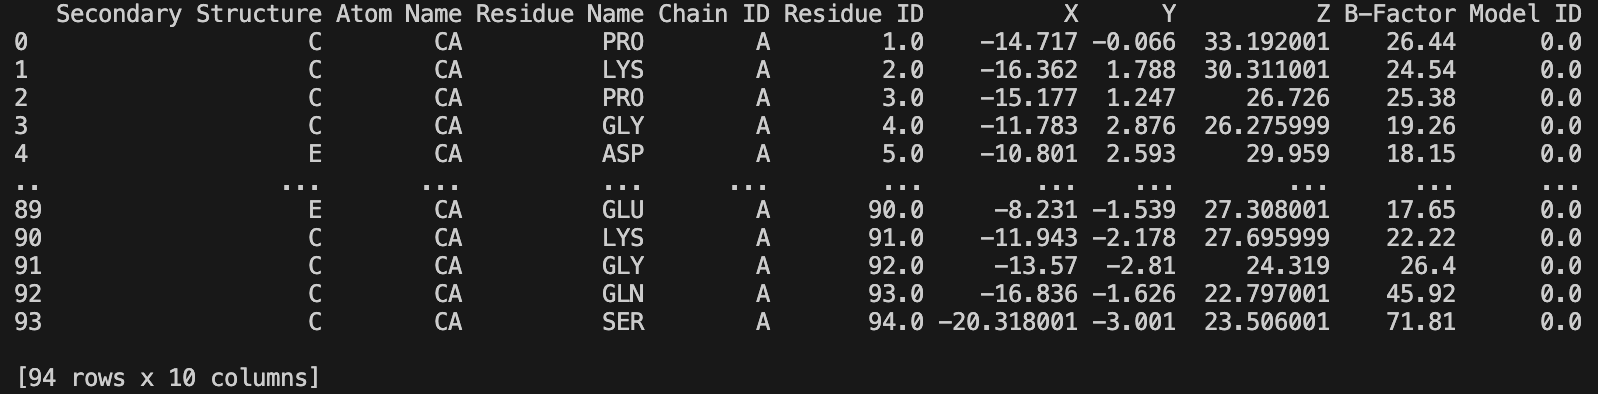
\includegraphics[width=0.8\textwidth]{/Users/enrico/PROTEINS/tesi/immagini_tesi_ingelse/Screenshot 2024-12-11 at 12.00.12.png}
    \caption{Dataset of 3LNX.}
\end{figure}

These dynamics are essential for understanding how allosteric sites are interconnected with the binding pockets involved in ligand binding. By perturbing these sites, particularly those in alpha-$\alpha$ regions, we observe targeted responses around the ligand site.\\
Choosing an appropriate connection radius is crucial for accurately capturing both local and long-range interactions between residues.\\
A too short radius may overlook long-range interactions, while a too long radius could obscure essential local interactions.\\
Based on literature and our findings, a connection radius of 8.0 nm was optimal, balancing the need to accurately reflect the protein’s mechanical and dynamic properties.

\begin{figure}[h!]
    \centering
    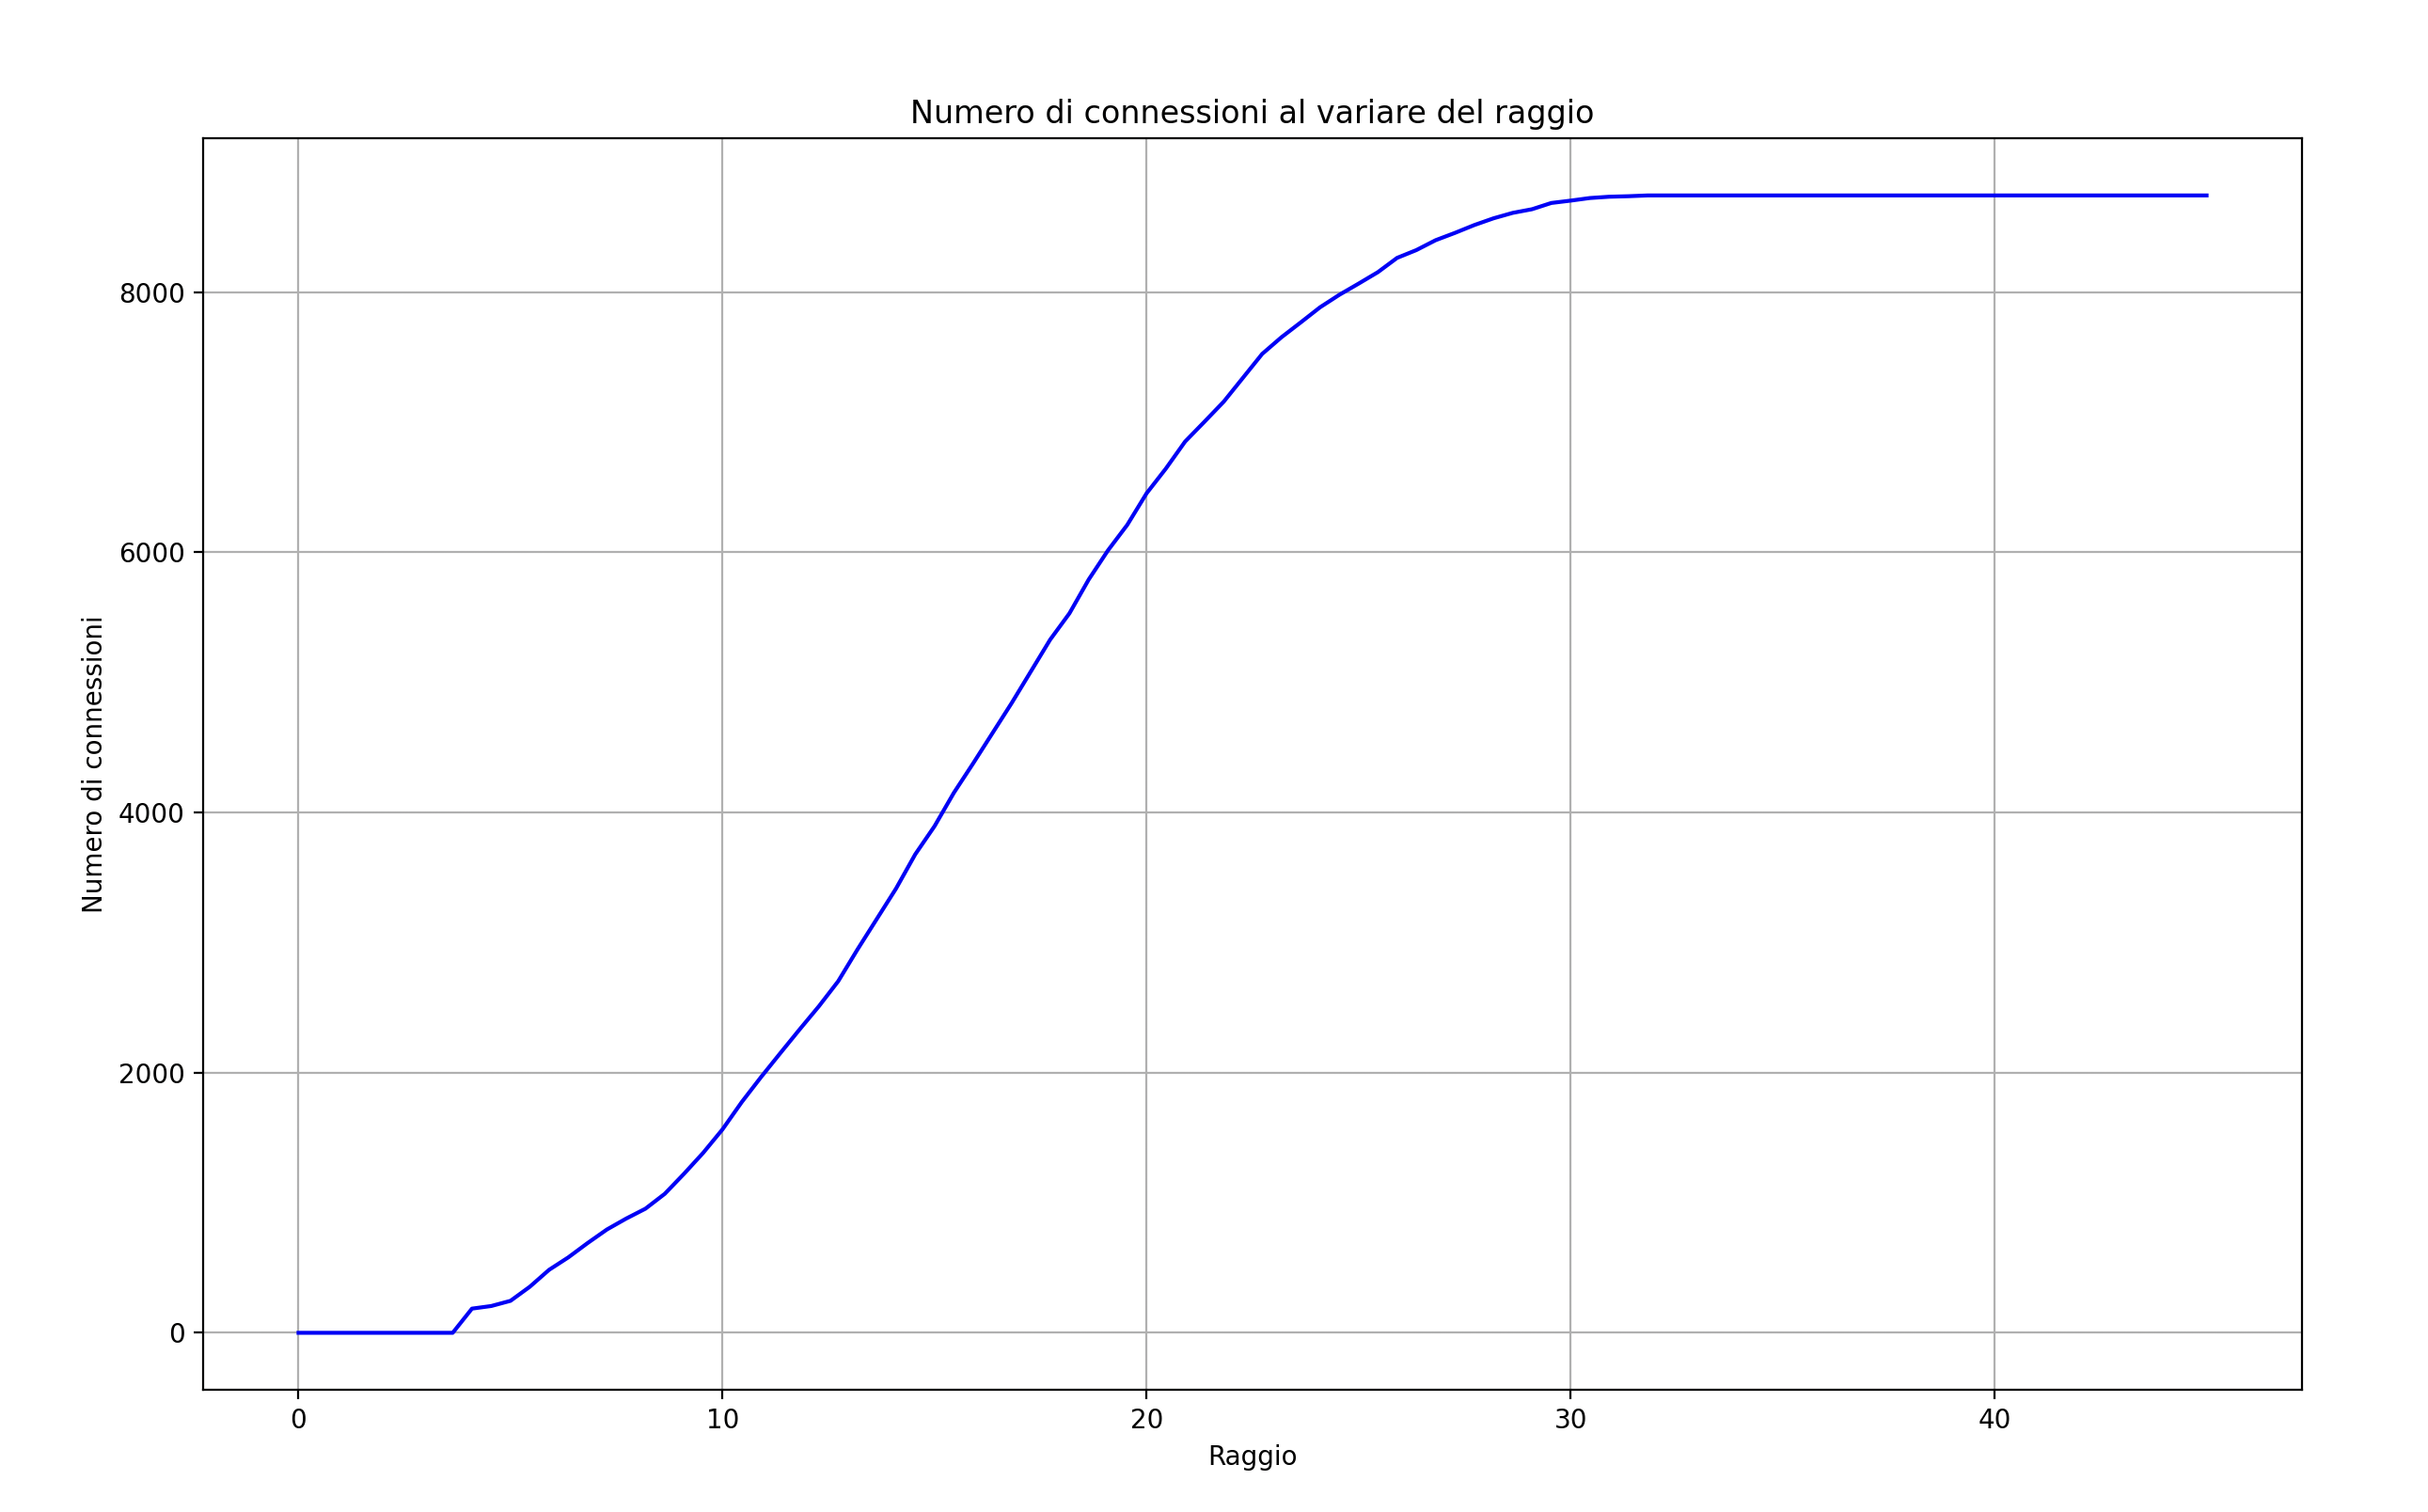
\includegraphics[width=0.8\textwidth]{/Users/enrico/PROTEINS/tesi/immagini_tesi_ingelse/Screenshot 2024-12-08 at 11.54.32.png}
    \caption{Number of links in function of the connection radius.}
\end{figure}

\begin{figure}[h!]
    \centering
    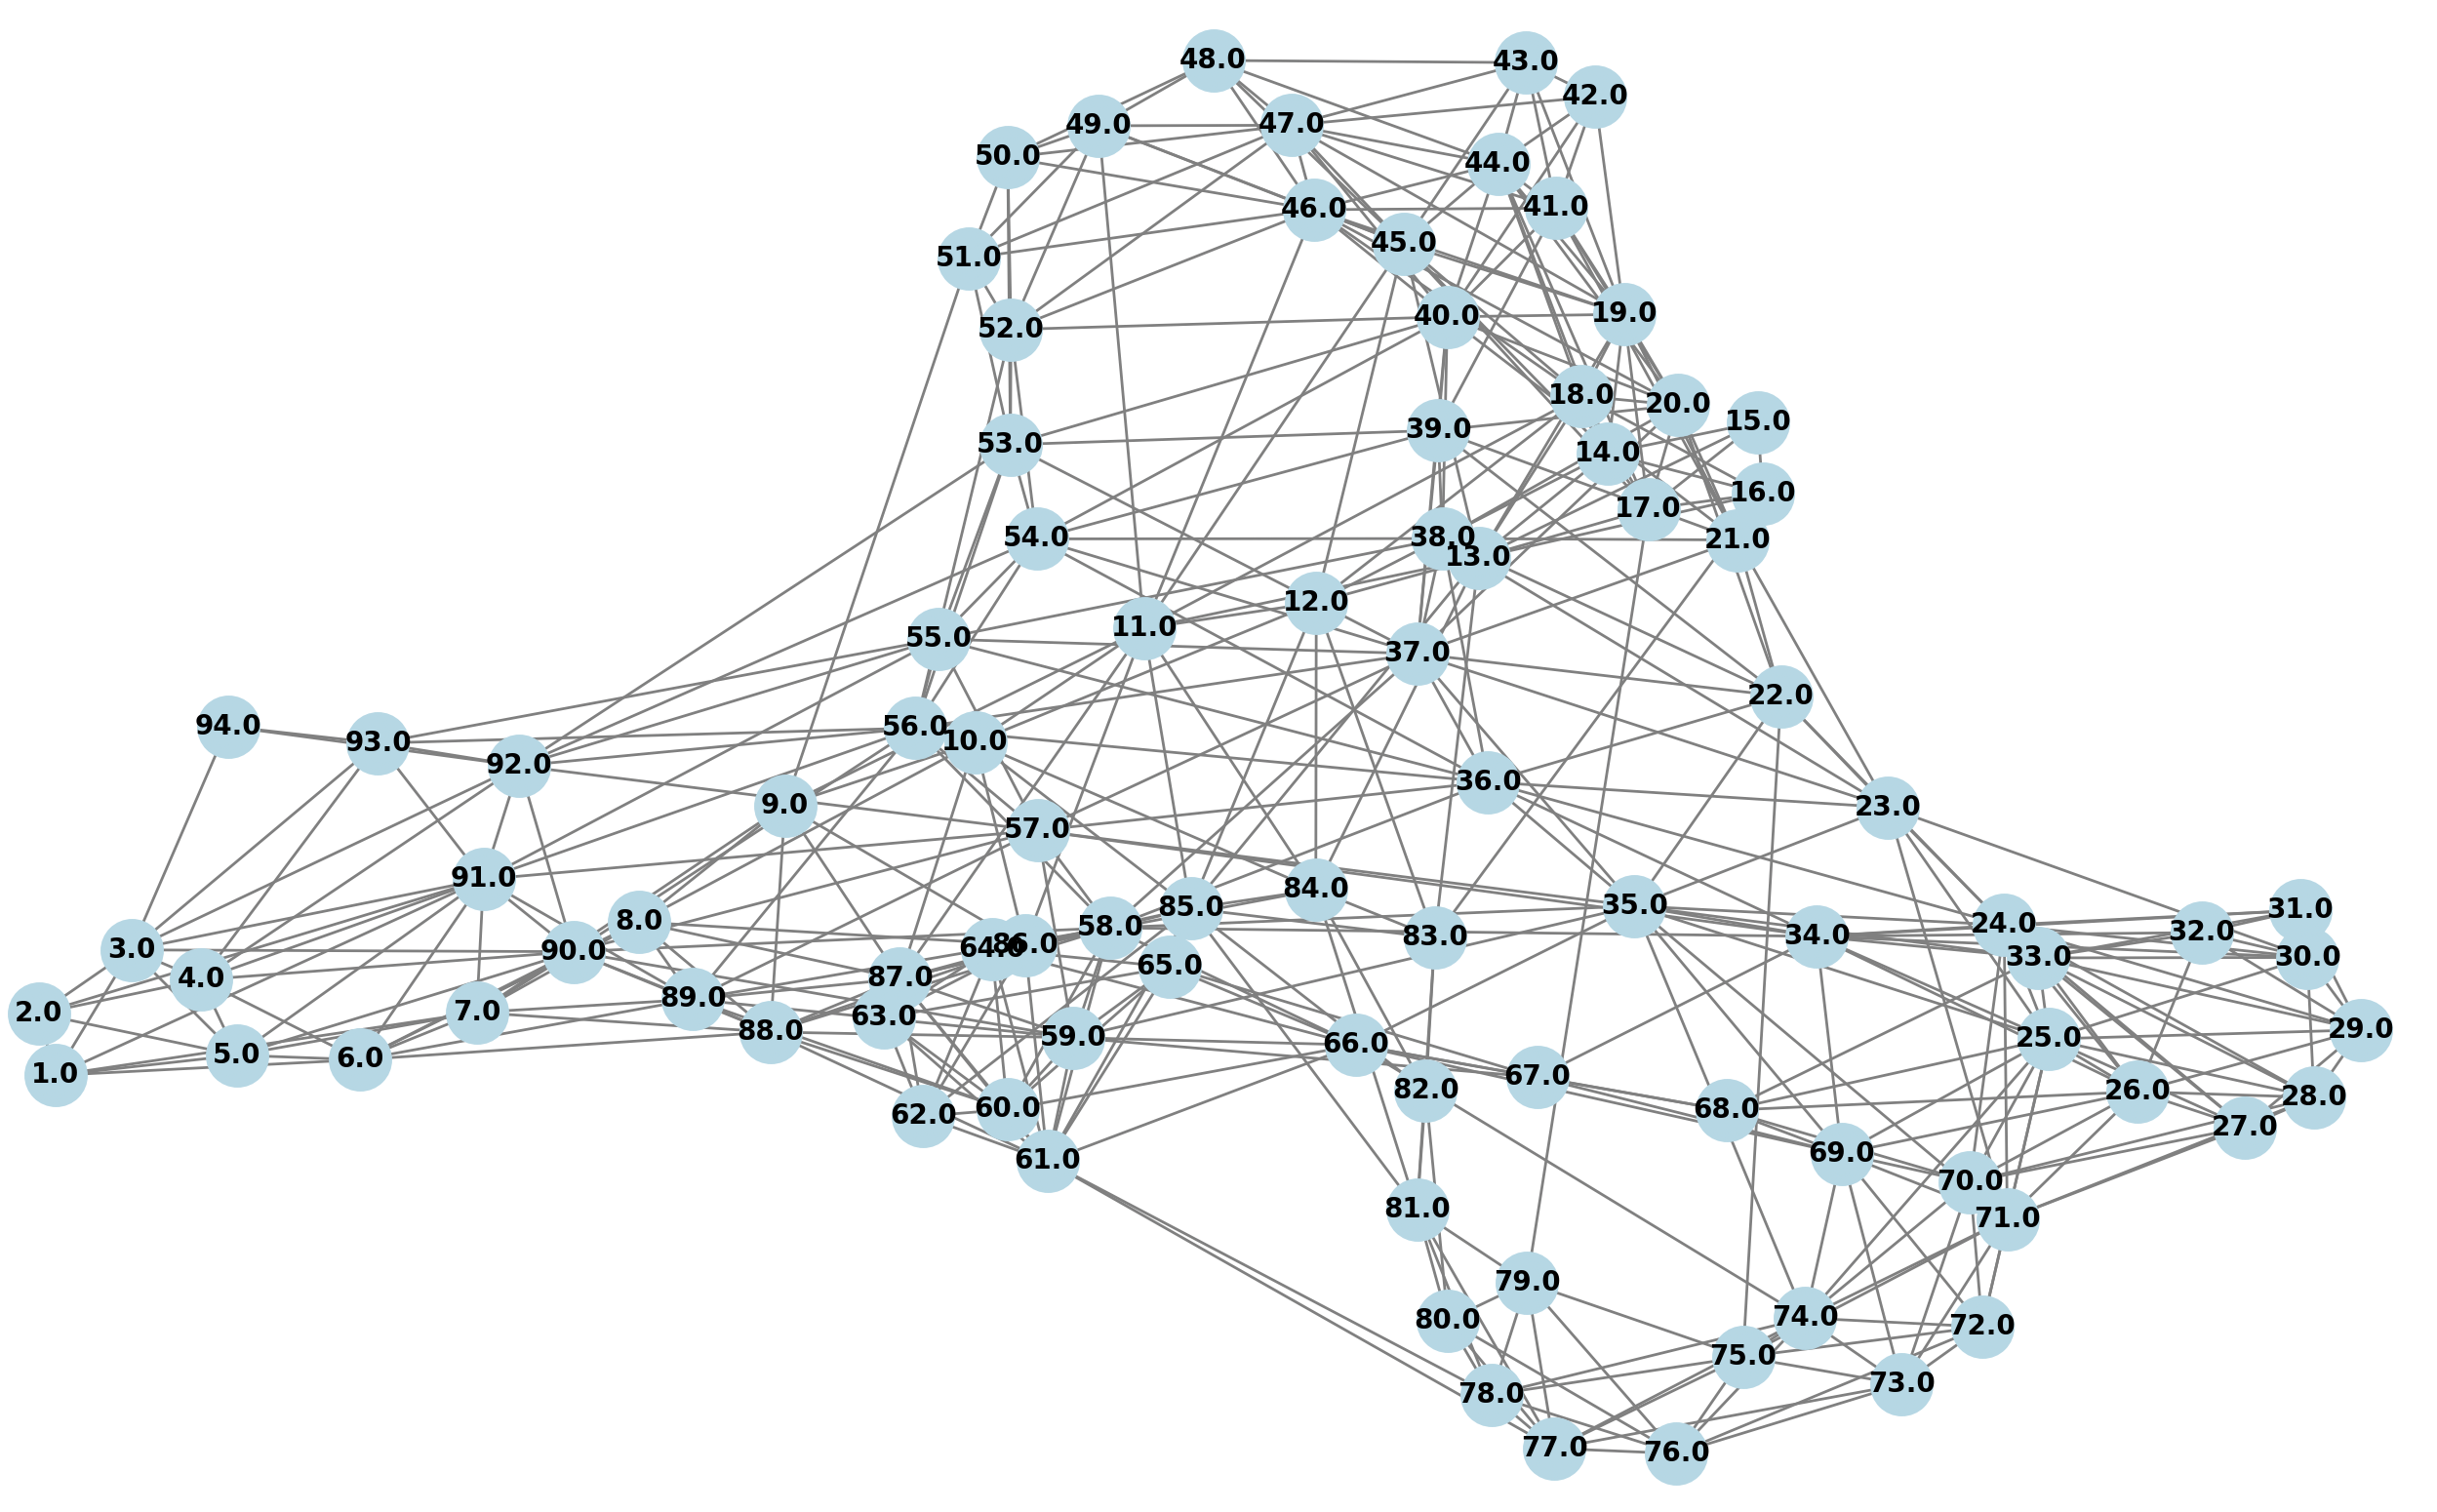
\includegraphics[width=0.8\textwidth]{/Users/enrico/PROTEINS/tesi/immagini_tesi_ingelse/Screenshot 2024-12-11 at 11.59.21.png}
    \label{fig:grafo_connessione}
    \caption{Bidirectional Graph obtained with radius of 8.0 nm.}
\end{figure}
Using this radius, we constructed a bidirectional graph, as shown, which captures the essential connectivity and dynamics within the protein structure.\\


By applying the Kirchhoff matrix formulation to the protein structure, we derive matrix K, which models the protein as a network of interactions. This matrix simplifies the complex web of protein interactions into pairwise connections, where the link weights represent the coupling strength between residues. Such simplification helps to visualize and analyze the dynamic properties of the protein but omits more complex interactions like solvation effects or multi-body interactions, which could also influence the protein's behavior.

The weights of the links are set based on the proximity and type of interaction between residues: typically, near neighbors connected by strong covalent bonds or dense non-covalent interactions (such as van der Waals forces and hydrogen bonds) are assigned a weight of 20. These interactions are considerably stronger, approximately 20 times greater, than those between more distantly connected residues, which receive a weight of 1. This weighting scheme reflects the biological reality where closer residues have stronger interactions that significantly influence protein dynamics.

Formally, the protein’s structure can be represented as a graph \( G = (V, E) \), where \( V \) is the set of vertices (residues), and \( E \) is the set of edges (connections between residues). The weight \( w(i, j) \) of the link between any two vertices \( i \) and \( j \) is defined as follows:
\[
w(i, j) =
\begin{cases}
20, & \text{if } i \text{ and } j \text{ are near neighbors}, \\
1, & \text{otherwise}.
\end{cases}
\]

\begin{figure}[h!]
    \centering
    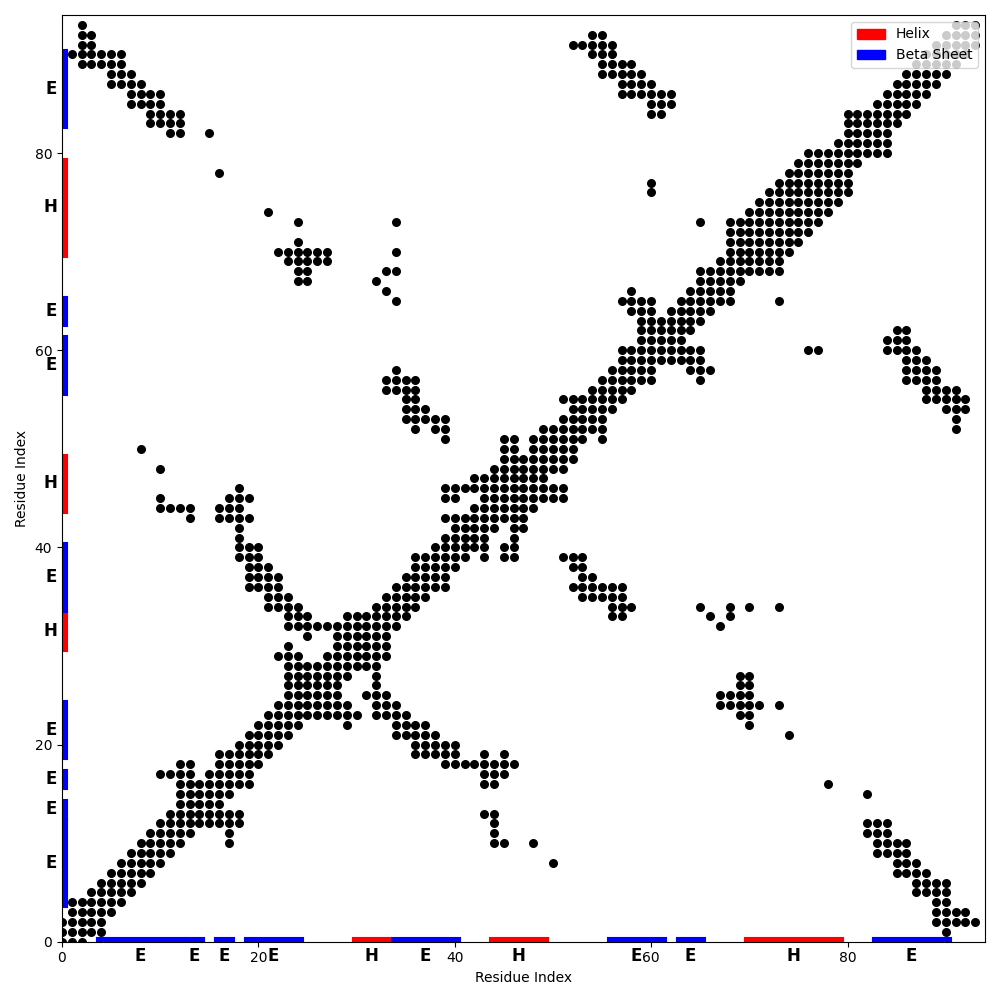
\includegraphics[width=0.8\textwidth]{/Users/enrico/PROTEINS/images/3LNX/contatti/Matrice di Kirchhoff della Proteina.png} 
    \caption{Kirchhoff Matrix of the protein structure.}
    \label{fig:kirchoff}
\end{figure}

This representation of the Kirchhoff matrix (\ref{fig:kirchoff}) visually encapsulates the connectivity and interaction patterns within the protein, highlighting how structural dynamics are influenced by both local and long-range interactions.

\\\\\\\\\\\\\\
We notice first that as expected the Kirchhoff matrix is symmetric and that the diagonal elements are all negative. \\
This is consistent with the physical interpretation of the matrix, where the diagonal elements represent the sum of the coupling strengths between a residue and all other residues in the protein. The negative sign indicates that the interactions are stabilizing, as expected in a protein structure. The off-diagonal elements represent the coupling between pairs of residues, reflecting the network of interactions that stabilize the protein's structure.\\
It is important to notice also that most of the links are between near residues, but we have also some cluster of links between distant residues. This is important because it means that the protein is not a simple chain of residues but it is a complex network of interactions.


Now we have to understand deeply how these interacting residues influence each other's dynamics.\\
For studying it we have to calculate the Covariance matrix.\\
at time 0:\\
The Covariance matrix at time 0 is defined as:
\[
C_{ij}(0) = \sum_{k=1}^N \frac{1}{\lambda_k} v_{ik} v_{jk}.
\]
The two figures illustrate the covariance matrices obtained from the protein structure, one only plotting the positive covariance and the other only plotting the negative covariance.\\
In the following figures we plot also the secondary structure (Helices: red; Beta Sheets: blue) and the kirchoff matrix.\\
\begin{figure}[h!]
    \centering
    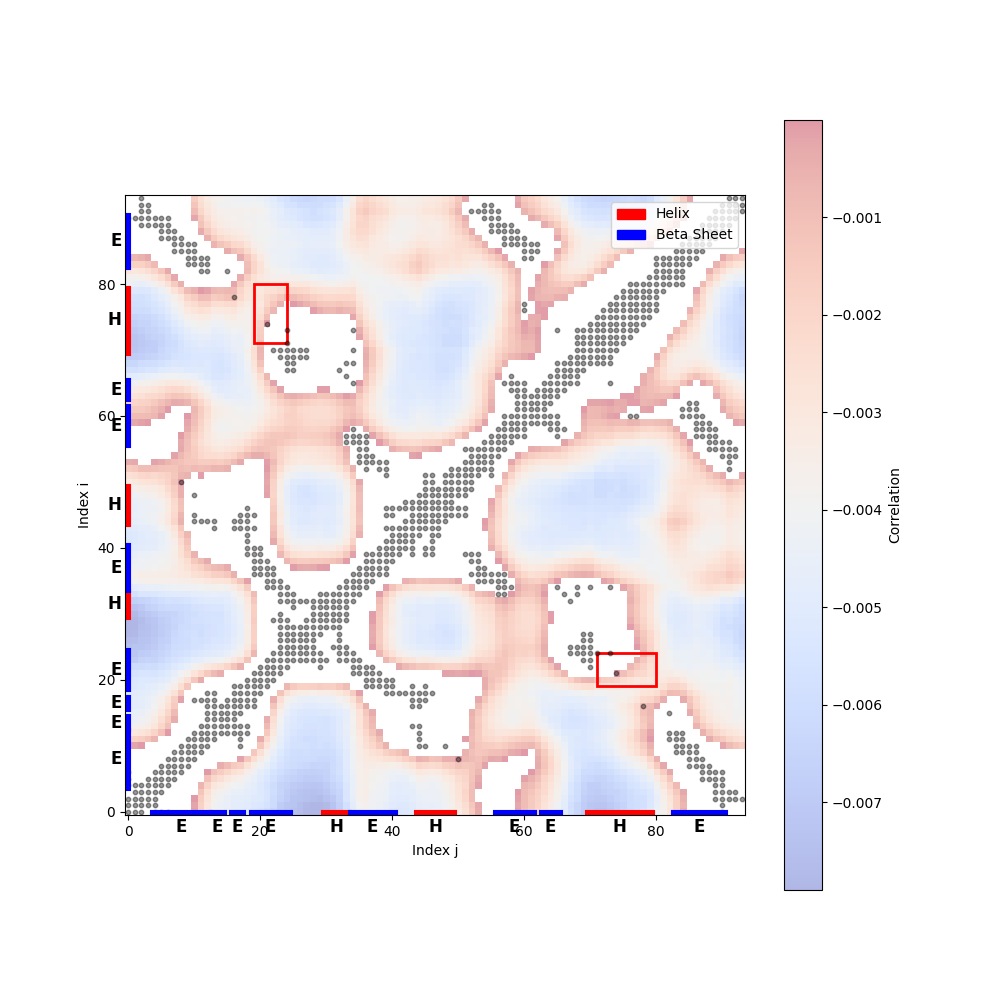
\includegraphics[width=0.8\textwidth]{/Users/enrico/PROTEINS/images/3LNX/Matrici/Correlation_MatrixNan_False.png}
    \caption{Negative covariance between residues at time 0.}
    \label{fig:Covariance_negative_figo}
\end{figure}

\begin{figure}[h!]
    \centering
    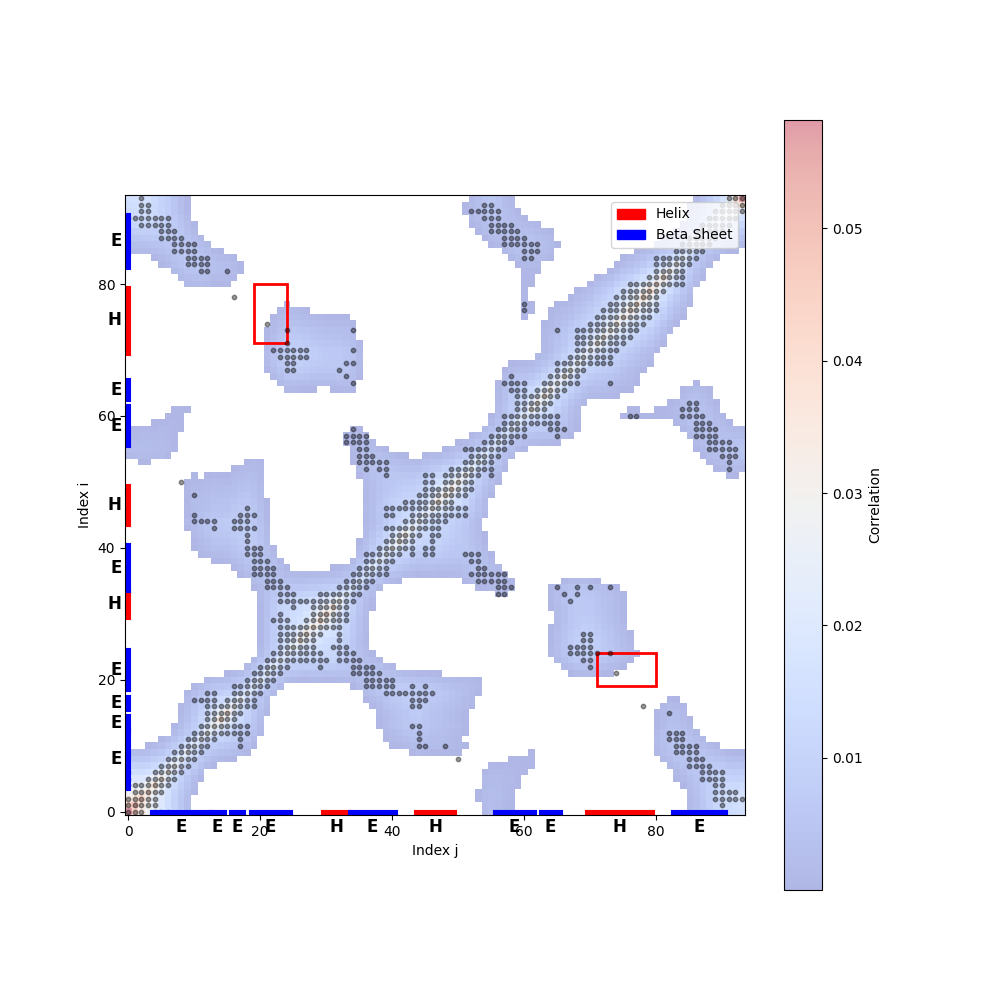
\includegraphics[width=0.8\textwidth]{/Users/enrico/PROTEINS/images/3LNX/Matrici/Correlation_MatrixNan_True.png}
    \caption{Positive covariance between residues at time 0.}
    \label{fig:Covariance_positive_figo}
\end{figure}
In these images we notice that we have positive Covariance where we have residues and negative Covariance where we don't have residues.
More distant is a region from the residues more negative will be the Covariance.\\
We can see also a cluster of the most postive corerlation along the diagonal.\\
So the Kirchhoff matrix directly influences the Covariance matrices by encoding the connectivity between residues. 


Now that we have the Covariance matrix at time 0, we can calculate the Beta Factors, wich are a critical measure of the protein's dynamic behavior.\\
They represent the atomic displacement and are useful for evaluating the protein's flexibility and stability and it also a tool for evaluating the theoretical model because we have experimental data of them.\\
Mathamically they are defined as:\\
$B_i = 8\pi^2 \langle C_{i,i} \rangle$ 

The plot above compares the experimental \( B \)-factors (blue curve), as we said in \eqref{beta} $B_i = 8\pi^2 C_{ii}$, with the predicted \( B \)-factors (red curve) along the residue index. \\
The \( B \)-factors represents the atomic displacement so they are a critical measure of the dynamic behavior of the protein structure. \\
They are also useful for testing the quality of the model.\\
\begin{figure}[h!]
    \centering
    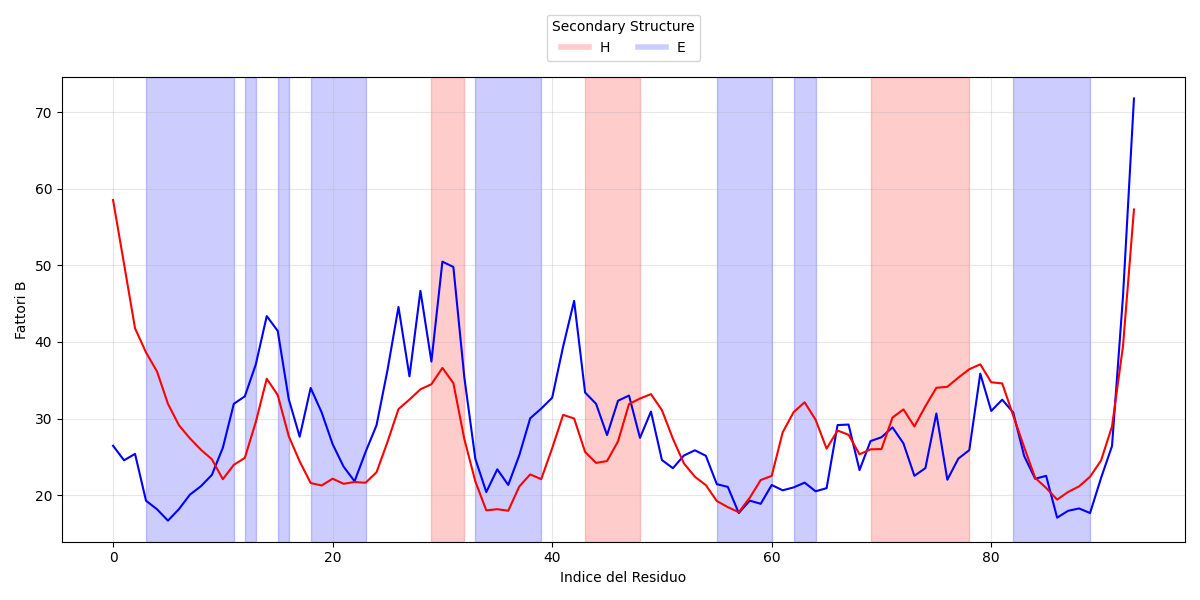
\includegraphics[width=0.8\textwidth]{/Users/enrico/PROTEINS/images/3LNX/beta_factors/Confronto_con_Struttura_Secondaria.png
    }
    \caption{Beta factors.}
\end{figure}
We see that the predicted \( B \)-factors generally follow the experimental trend, demonstrating the effectiveness of the model in capturing the dynamics of the protein.\\
Discrepancies between the predicted and experimental curves are visible in certain regions; these deviations may be due to limitations in the Kirchhoff matrix approximation or oversimplified assumptions in the modeling process.\\
To evaluate the model performance we have to define the following metrics RMSE e MAE:
\[
\text{RMSE} = \sqrt{\frac{1}{n} \sum_{i=1}^n (y_i - \hat{y}_i)^2}
\]

\[
\text{MAE} = \frac{1}{n} \sum_{i=1}^n |y_i - \hat{y}_i|
\]
Where \(y_i\) are observed values, \(\hat{y}_i\) are predicted values.
The main difference from RMSE and MAE is that RMSE gives more weight to large errors, while the MAE gives equal weight to all errors.\\
Now finaly with these quantitative metrics we can evaluate the model performance:\\
\begin{table}[h!]
    \centering
    \begin{tabular}{|c|c|}
    \hline
    \textbf{Metric} & \textbf{Value} \\ \hline
    RMSE & 8.5200 \\ \hline
    MAE  & 6.4146 \\ \hline
    \end{tabular}
    \caption{Model Performance Metrics}
    \label{tab:model_metrics}
\end{table}
This table shows the RMSE and MAE values for the model and show the model is good to predict the beta factors behavior.\\
It is clear that we can improve the model and it is possible to obtain more accurate predictions.\\
Now let's valuate if the model can catch the allosteric dynamics of the protein.\\
\newpage
















\section{Causal indicators in time}
\noindent In this section we will focus on the causal indicators in time and between residues.\\
Understanding the dynamic interactions within the protein structure requires analyzing how causal indicators like Covariance and Response behave over time, supplemented by Transfer Entropy to gauge information flow.\\
In this way we have deeply view of allosteric mechanism of the protein.\\
Let's start with the Covariance in time.\\
The Covariance between residues at time \(t\) is defined as:
\[
C_{ij}(t) = \sum_{k=1}^N v_{ik} v_{jk} \frac{e^{-g \lambda_k t}}{g \lambda_k} ,
\]
\begin{figure}[h!]
    \centering
    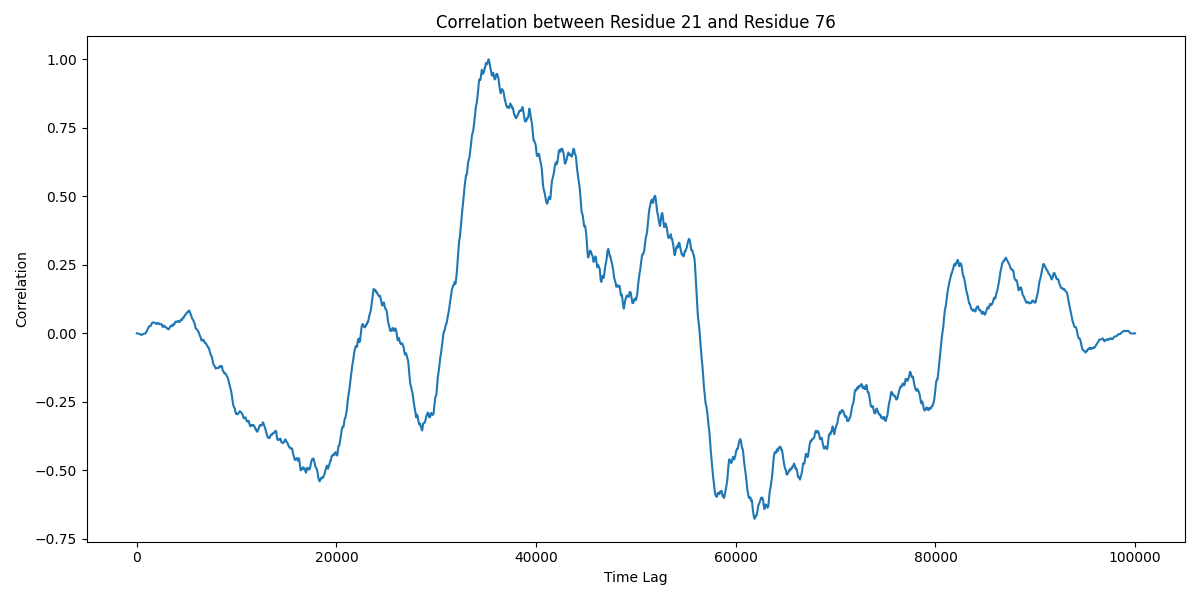
\includegraphics[width=0.8\textwidth]{/Users/enrico/PROTEINS/images/3LNX/Multiple_time_Correlation/Correlation.png}    
    \caption{Covariances in time.}
\end{figure}
This behavior is coherent with what expected, the Covariance decay over time, indicating a loss of direct dynamic influence as time progresses.\\
Moreover Covariance values vary significantly between residue pairs, reflecting differences in their initial dynamic coupling.\\
Finally residue pairs closer in space tend to show higher initial Covariances compared to more distant pairs.\\
The decay in Covariance is largely attributable to the intrinsic thermal motions within the protein structure.\\
Each residue in a protein is subject to thermal vibrations and random collisions with surrounding molecules, which contribute to the diffusion of any initial localized perturbations across the protein structure.\\
Over time, these random motions cause the initial correlations in residue movements to dissipate, leading to a decrease in Covariance values.\\
From a biological perspective, the decay of Covariance over time can be indicative of the protein’s ability to return to a stable state after undergoing a conformational change.\\
This is crucial for protein functionality, as proteins often need to respond dynamically to cellular signals or environmental changes and then return to their baseline state to be ready for subsequent interactions.\\
The rate and pattern of Covariance decay can therefore provide insights into the resilience and stability of protein structures, as well as their capability to undergo conformational changes necessary for biological activity.\\
Moreover, understanding the decay patterns of Covariance can help in identifying regions within the protein that are particularly flexible or rigid. 
Regions with slower decay rates may indicate domains of the protein that maintain their conformational relationships over longer periods, which could be critical for maintaining the structural integrity necessary for specific biological functions. Conversely, areas with rapid Covariance decay might be more flexible, allowing the protein to adapt its shape for different functional interactions.\\

\newpage
Now we can analyze the response in time.\\
The response metric is crucial for understanding how protein residues react over time to specific perturbations.\\
Unlike covariance, which can fluctuate between positive and negative values reflecting the strength and direction of coupling, the response is inherently positive, emphasizing the accumulation of effects from the initial perturbation:
\[
R_{ij}(t) = \frac{1}{N}+{\sum_{k=1}^N  v_{ik} v_{kj} e^{-g \lambda_k t}}.
\]
This mathematical representation highlights how the response function quantifies the influence of dynamic changes across the protein structure as they decay over time.
\begin{figure}[h!]
    \centering
    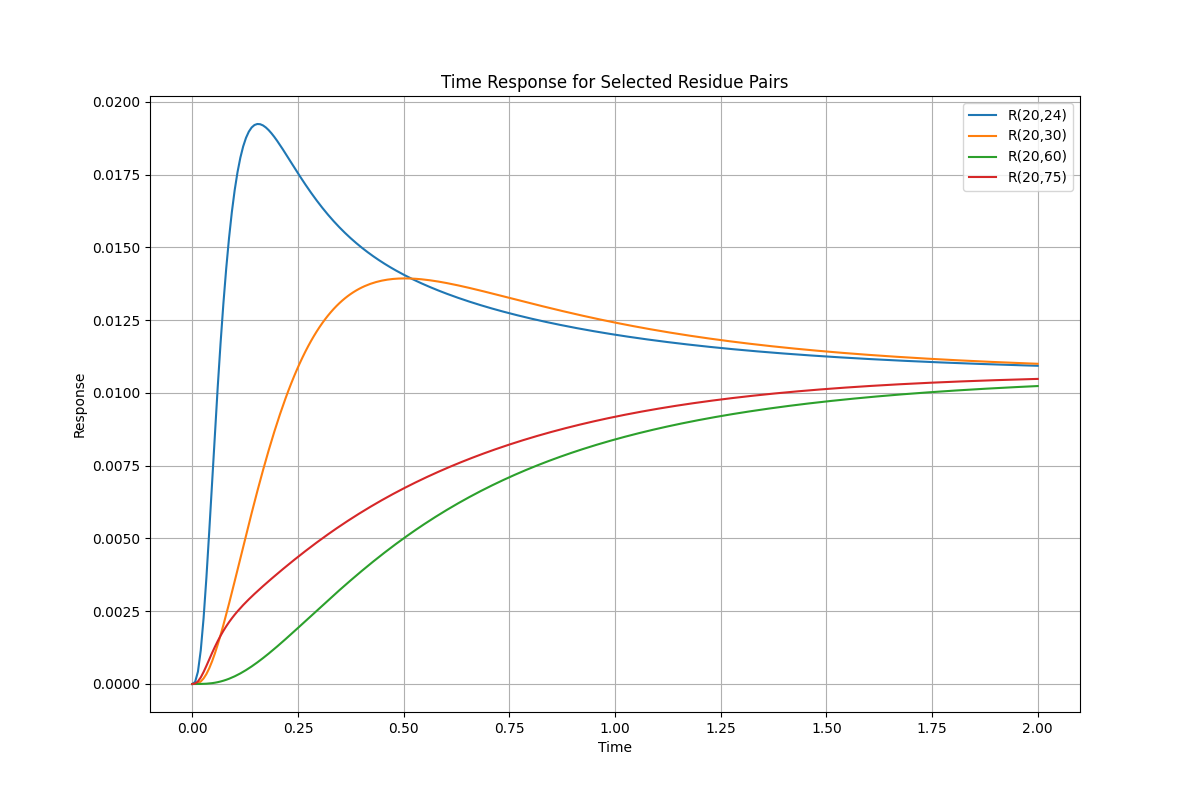
\includegraphics[width=0.8\textwidth]{/Users/enrico/PROTEINS/images/3LNX/Multiple_time_resposne/risposte.png}    
    \caption{Responses in time, illustrating a sharp initial rise and gradual decay, reflecting dynamic adaptations within the protein structure.}
\end{figure}
This behavior is coherent with what expected, the response decays over time, indicating a loss of direct dynamic influence as time progresses. \\
Also, we notice that when covariance can be positive or negative, the response is always positive, starting from 0 and reaching the value of 1/N.\\
The responses exhibit a sharp rise initially, which is then followed by a gradual decay.\\
Residue pairs closer to the source of perturbation (spatially proximal) show a more pronounced and faster response.\\
This proximity effect highlights the importance of spatial relationships in protein dynamics, where residues near the source of perturbation are more immediately and strongly affected.\\
A peak is observed at an intermediate time point for most residue pairs, indicating a time of maximum information transfer.\\
This peak represents the critical moment when the effects of the perturbation are most acutely felt throughout the protein, suggesting key points of allosteric control or regulatory interaction within the protein structure (We will soon explore this in detail).\\
Understanding these peaks can provide insights into the timing and extent of protein responses that are crucial for biological functions such as enzyme activation or signaling pathways.\\
        
\newpage
Now we can analyze the transfer entropy in time:
\[
TE_{j \to i}(t) = -\frac{1}{2} \ln {(1 - \frac{\alpha_{ij}(t)}{\beta_{ij}(t)})},
\]
where:
\[
\alpha_{ij}(t) = \left[C_{ii}(0)C_{ij}(t) - C_{ij}(0)C_{ii}(t)\right]^2,
\]
\[
\beta_{ij}(t) = \left[C_{ii}(0)C_{jj}(0) - C_{ij}^2(0)\right]\left[C_{ii}^2(0) - C_{ii}^2(t)\right].
\]
This formulation quantifies the directional non linear information flow from residue \( j \) to \( i \) over time, reflecting how changes in covariance impact the dynamics of information transfer within the protein.
\begin{figure}[h!]
    \centering
    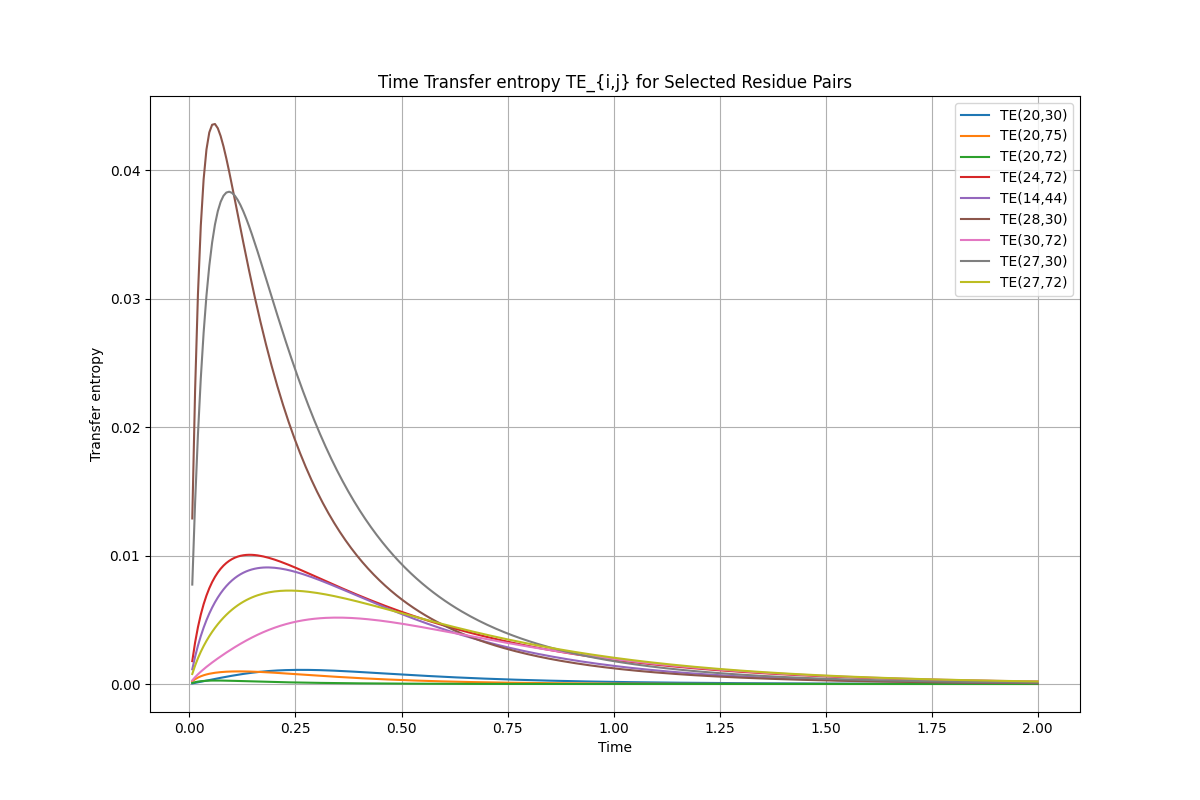
\includegraphics[width=0.8\textwidth]{/Users/enrico/PROTEINS/images/3LNX/Multiple_time_Correlation/entropy.png}
    \caption{Transfer entropy over time, highlighting critical moments when the information flow peaks, indicating significant regulatory interactions within the protein structure.}
\end{figure}
\newpage
In this analysis, we observe that a peak is seen at an intermediate time point for most residue pairs, signaling a time of maximum information transfer.\\
This peak is crucial as it may indicate a pivotal moment when one residue exerts a strong influence over another, potentially triggering a significant functional response or regulatory mechanism.\\
Moreover, the magnitude of transfer entropy varies, reflecting differences in the strength of directional coupling between pairs. Residue pairs with high initial connectivity, which are typically spatially closer within the protein structure, exhibit stronger peaks compared to those more distant.\\
This pattern underscores how structural proximity within a protein can significantly enhance the efficiency and impact of informational transfer, aligning with known biological principles that spatially close residues often participate in more direct and influential interactions.\\


\newpage
Now that we understood the casual indicators in time we can finaly analyze the causal indicators between residues to identify the allosetric mechanism.\\
This is the main section of our work in which we will try to understand the allosteric mechanism of the protein and understand for real if the model explain in a good way the protein dynamics.\\
As we said before if the graph of the proteins were random we will expected random interaction.\\ 
For seeing if our model is in according with the real world results if we perturb the allosteric sites, situated in according with paper \cite{ref15} in all the alpha-$\alpha$ and alpha-$\gamma$ helices, we will expected that the signal will propagate along the protein structure for reaching the active sites, around beta-$\beta$ and Alpha-$\alpha$.\\
To analyze our system, it is essential to focus on timescales around the characteristic time \(\tau\). \\
In fact if the time \(t\), in which we analyze the system, is too short so we don't see in a right way the propagation, in other hand if the time is too long we don't see the relaxation of the system.\\
So to determine the characteristic time \(\tau\) of the system, we have to analyze the autocorrelation normalized function \(C_{i,i}(t)\)/\(C_{i,i}(0)\) between all residues for all relevant times \(t\). \\
The idea is that the mean of typical decay time is the characteristic time \(\tau\) of my system.\\
Mathematically for each index \(i\)  will take the autocorrelation normalized \(C_{i,i}(t)\)/\(C_{i,i}(0)\) when they are equal to \(e^{-1}\) of their initial values. These times are the \(t_i\) for every residues.\\
Now i have an histogram  of times and taking the mean of this vlaues i will obtain my characteristic time \(\tau\).\\
We estimated a time \(\tau\) of 0.1842 ns.\\
\begin{figure}[h!]
    \centering
    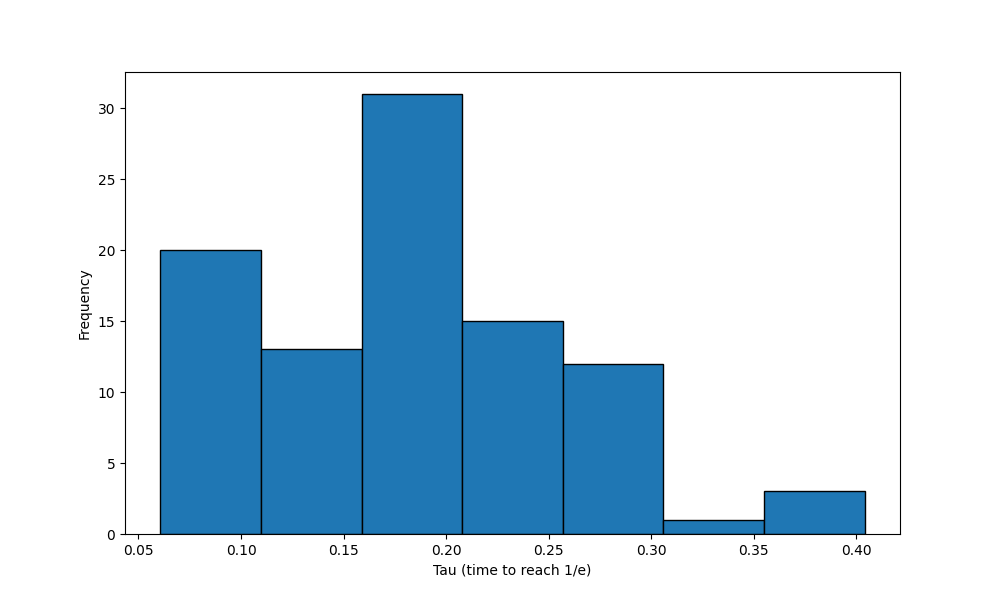
\includegraphics[width=0.8\textwidth]{/Users/enrico/PROTEINS/images/3LNX/2_temperature_cutoff/Stima_tau/tau_histogram.png}
    \caption{Hisotgram of \(t_i\).}
\end{figure} 
\begin{figure}[h!]
    \centering
    \includegraphics[width=0.8\textwidth]{/Users/enrico/PROTEINS/images/3LNX/Stima_tau/autoCorrelation_fits.png}
    \caption{Normalized autocorrelations of all residues with also a sketched plot of the autocorrlation with the fitted tau.}
\end{figure}

\newpage
\newpage
\section{Causal indicators between residues}
Now we can analyze all the causal indicators between the allosteric sites and all other residues at the three times at [\(\tau\)-0.5*\(\tau\), \(\tau\), \(\tau\)+0.5*\(\tau\)].\\
Our goal is to catch a link between the allosteric sites in the secondary structure alpha-$\alpha$ and alpha-$\gamma$ and the binding pocket between beta-$\beta$ and alpha-$\alpha$.\\
To do it we have to compute the covariance, the response and the trasnfer entropy between residues.\\

This is the plot of the Covariance between the specific allosteric sites at time \(\tau\) and all the residues:
\begin{figure}[h!]
    \centering
    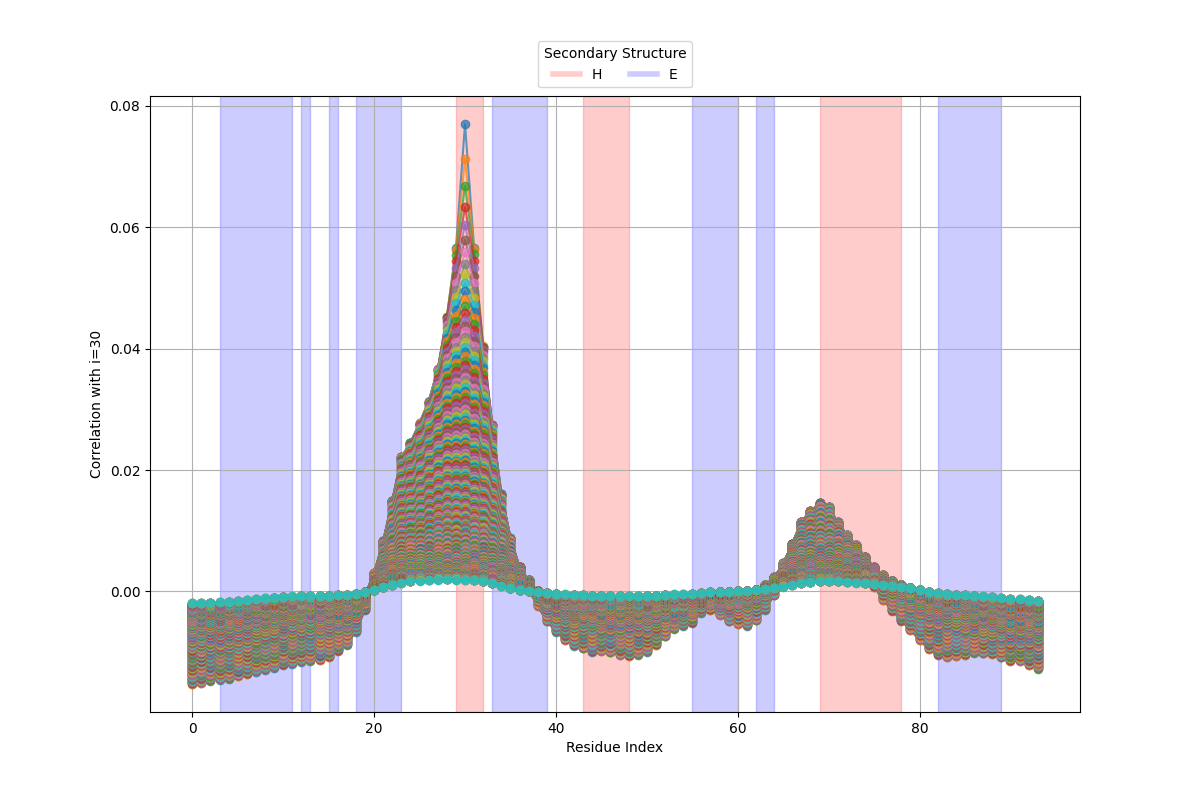
\includegraphics[width=0.8\textwidth]{/Users/enrico/PROTEINS/images/3LNX/Time_indicators/Residual Correlation C_ij for i=30 as a function of j at time index 0.png}
    \caption{Covariance of 31-th residue at \(\tau\), showing localized interaction peaks indicative of dynamic communication pathways.}
    \label{fig:Covariance of 31-th residue}
\end{figure}
\newpage
In the Covariance of residue 31 \ref{fig:Covariance of 31-th residue} there are a high Covariance observed near the binding pocket,as we expected, particularly between the alpha-$\alpha$ and beta-$\beta$ regions, and another allosteric site in the alpha-$\gamma$ helix, highlights regions of significant allosteric communication.\\
Moreover we see also strong values of covariance in the head and in the tail of the protein, probability caused by spourious interactions. 
We will use following the others causal indicators to understand it better.\\

\begin{figure}[h!]
    \centering
    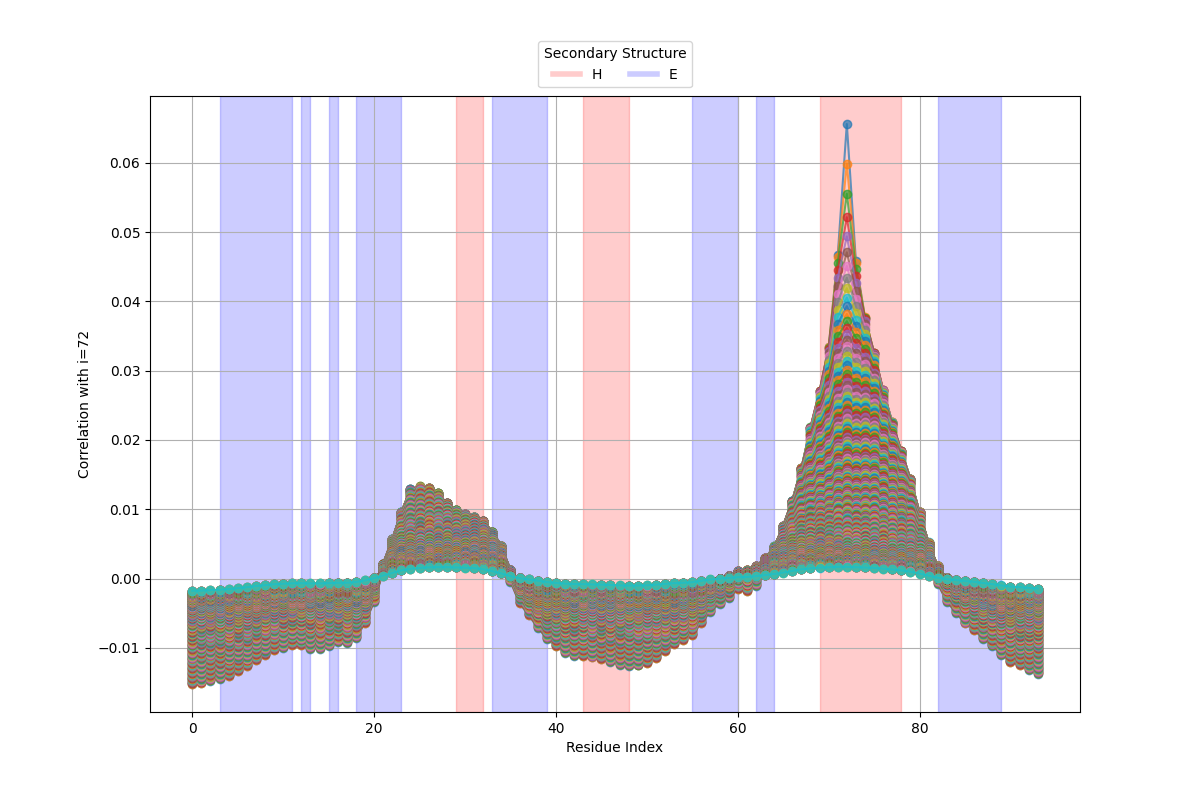
\includegraphics[width=0.8\textwidth]{/Users/enrico/PROTEINS/images/3LNX/Time_indicators/Residual Correlation C_ij for i=72 as a function of j at time index 0.png}
    \caption{Covariance of 73-rd residue at \(\tau\), emphasizing the inter-domain communication crucial for protein functionality.}
    \label{fig:Covariance of 73-rd residue}
\end{figure}
Now we analyze the Covariance of residue 73 \ref{fig:Covariance of 73-rd residue}.\\
We notice a distinct peak around the 73-rd residue, due to the locatility, and other strong signals especially in regions like the beta-$\beta$-strand and alpha-$\alpha$-helix near the binding pocket.\\
Also here we see strong values of covariance in the head and in the tail of the protein.\\

For both the analysis we see that the Covariance is high in the binding pocket, between the beta-$\beta$ and alpha-$\alpha$ regions, and in the allosteric sites in the alpha-$\alpha$ and alpha-$\gamma$ helices.\\
This is coherent with what we expected, the signal propagate from the allosteric sites to the binding pocket.\\







Now to do a deeper analysis we can calculate the response of the protein to the perturbation of the allosteric sites.\\
When perturbing the 31-th residue, a significant response is observed across various regions of the protein. 
This is visualized in the response data presented below:
\begin{figure}[h!]
    \centering
    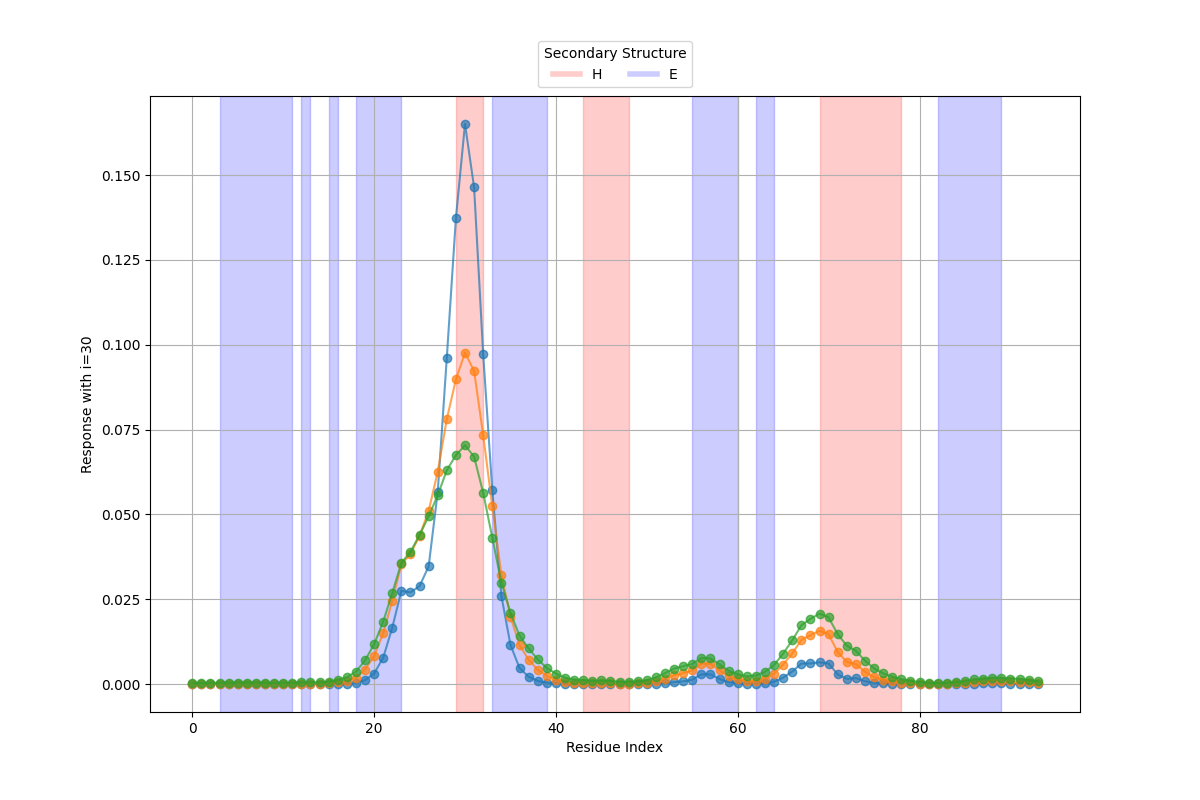
\includegraphics[width=0.8\textwidth]{/Users/enrico/PROTEINS/images/3LNX/Time_indicators/Time Response R_ij for i=30 as a function of j at time index 0.png}
    \caption{Dynamic response observed from perturbating the 31-th residue, illustrating signal propagation through alpha-$alpha$ helical regions.}
    \label{fig:resp31}
\end{figure}
\newpage
From the response \ref{fig:resp31} it is clear a response in the beta-$\beta$ sheet, in the alpha-$\alpha$ helix and at the start of alpha-$\gamma$ helix; indicating a strong propagation of the signal from the allosteric site directly to the binding pocket. \\
Moreover this result is particularly informative as it helps refute previous hypotheses suggesting significant signaling activities in the head and tail regions of the protein, where high covariance was initially observed. \\
In fact while those regions exhibit covariance, they do not necessarily contribute to causal interactions related to the protein's active functions. \\
But we have to note that while we observe these specific responses they do not alone confirm causality, however, the strong correlation between site-specific perturbation and localized response does support the hypothesis of these regions being critically involved in the allosteric mechanism.\\
With these insights, we can now present a new representation of the causal interactions within the protein eliminating the spurious relationship.\\
\begin{tikzpicture}[node distance=2cm]

    % Nodes for perturbation and regions
    \node (alphaalpha) [draw, rectangle, text centered, minimum height=1cm, minimum width=2cm] {Perturbazione alpha-$\alpha$ helix};
    
    % Nodes for regions below alpha-alpha, aligned horizontally with extra spacing
    \node (binding) [below of=alphaalpha, draw, rectangle, text centered, minimum height=1cm, minimum width=2.5cm, xshift=-6cm, yshift=-1cm] {Binding Pocket}; 
    \node (alphaGamma) [below of=alphaalpha, draw, rectangle, text centered, minimum height=1cm, minimum width=2.5cm, xshift=6cm, yshift=-1cm] {alpha-$\gamma$};
    
    
    % Draw arrows from alpha-alpha to each region
    
    \draw[->] (alphaalpha) -- (binding);
    \draw[->] (alphaalpha) -- (alphaGamma);

\end{tikzpicture}\\


Now we analyze the response of the protein to the perturbation of the 73-rd residue:
\begin{figure}[h!]
    \centering
    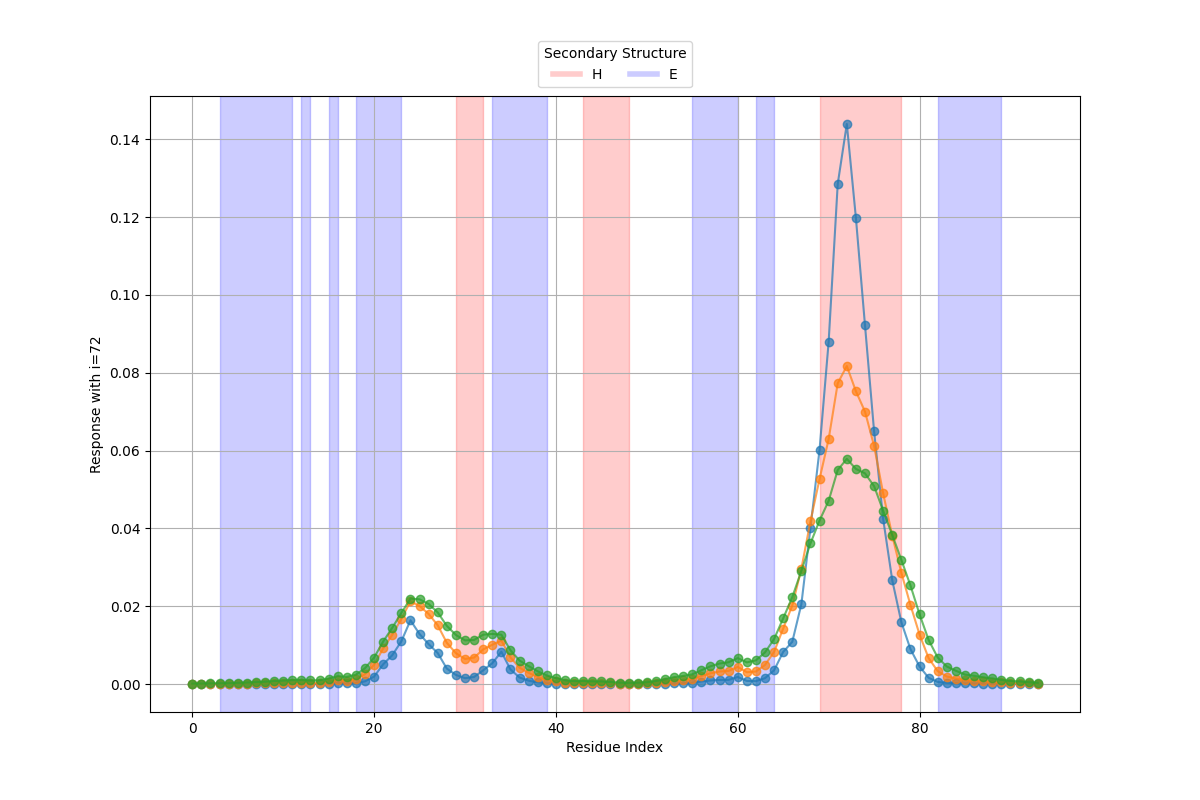
\includegraphics[width=0.8\textwidth]{/Users/enrico/PROTEINS/images/3LNX/Time_indicators/Time Response R_ij for i=72 as a function of j at time index 0.png}
    \caption{Dynamic response observed from perturbing the 73-rd residue, highlighting the interaction with critical functional regions of the protein.}
    \label{fig:resp73}
\end{figure}
Perturbing the 73-rd residue we note a response in the binding pocket and other significant interactions in the alpha-$\beta$ and moderate responses in the beta-$\gamma$ regions.\\
That suggest the existence of the allosteric mechanism which we expect.\\
The alpha-$\beta$ and beta-$\gamma$ regions, showing varied levels of response, are likely involved in stabilizing the protein upon ligand binding or release.\\ 
To better represent these findings, we update our causal interaction diagram to emphasize the newly identified pathways of influence.\\
\begin{tikzpicture}[node distance=2cm]

    % Nodes for perturbation and regions
    \node (alphaalpha) [draw, rectangle, text centered, minimum height=1cm, minimum width=2cm] {Perturbazione alpha-$\gamma$ helix};
    
    % Nodes for regions below alpha-alpha, aligned horizontally with extra spacing
    \node (binding) [below of=alphaalpha, draw, rectangle, text centered, minimum height=1cm, minimum width=2.5cm, xshift=-6cm, yshift=-1cm] {Binding Pocket}; 
    \node (alphaGamma) [below of=alphaalpha, draw, rectangle, text centered, minimum height=1cm, minimum width=2.5cm, xshift=6cm, yshift=-1cm] {alpha-$\alpha$};
    
    
    % Draw arrows from alpha-alpha to each region
    
    \draw[->] (alphaalpha) -- (binding);
    \draw[->] (alphaalpha) -- (alphaGamma);

\end{tikzpicture}


\newpage
To have a deeper point of view of causality mechanism and to undestand the directional flux of information within the protein we have now to study the transfer entropy.
We begin by examining the active transfer entropy from the allosteric sites to the other residues, represented as \( T_{\text{allosteric site}, j}\).
\begin{figure}[h!]
    \centering
    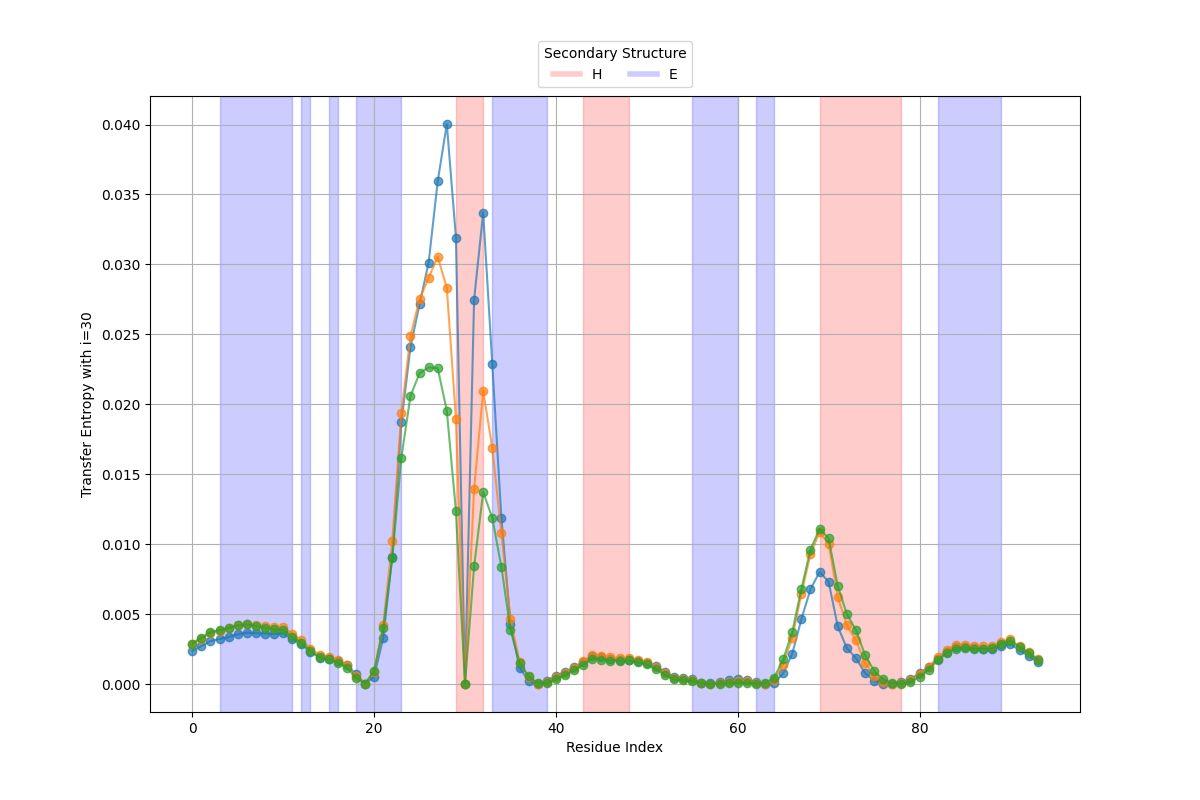
\includegraphics[width=0.8\textwidth]{/Users/enrico/PROTEINS/images/3LNX/Time_indicators/Transfer Entropy TE_ij for i=30 as a function of j at time index 0.png}
    \caption{Transfer Entropy j->31 (T_{31,j}).}
    \label{fig:TE31}
\end{figure}
Analyzing the images \ref{fig:TE31} we observe that signals are notably propagated within the binding pocket and the alpha-$\gamma$ helix.\\
The pattern revealed is quite similar to the response data.\\
To visualize these findings, we maintain our current graph of causal relations, which clearly shows the directional influence between identified regions:
\begin{tikzpicture}[node distance=2cm]
    \node (alphaalpha) [draw, rectangle, text centered, minimum height=1cm, minimum width=2cm] {Perturbation alpha-$\alpha$ helix};
    \node (binding) [below of=alphaalpha, draw, rectangle, text centered, minimum height=1cm, minimum width=2.5cm, xshift=-6cm, yshift=-1cm] {Binding Pocket}; 
    \node (alphaGamma) [below of=alphaalpha, draw, rectangle, text centered, minimum height=1cm, minimum width=2.5cm, xshift=6cm, yshift=-1cm] {alpha-$\gamma$};
    
    \draw[->] (alphaalpha) -- (binding);
    \draw[->] (alphaalpha) -- (alphaGamma);
\end{tikzpicture}\\

Similar findings are noted for the 73rd residue:
\begin{figure}[h!]
    \centering
    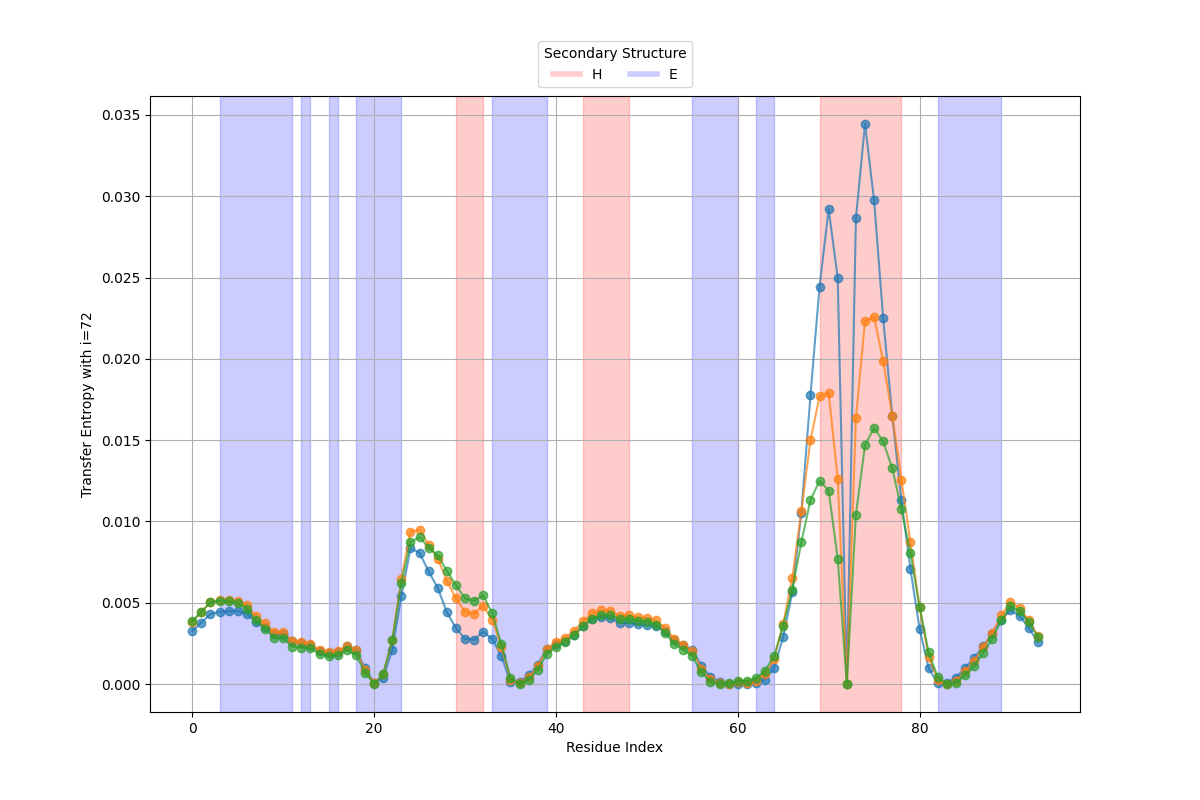
\includegraphics[width=0.8\textwidth]{/Users/enrico/PROTEINS/images/3LNX/Time_indicators/Transfer Entropy TE_ij for i=72 as a function of j at time index 0.png}
    \caption{Transfer Entropy j->73 (T_{73,j}).}
    \label{fig:TE73}
\end{figure}
This analysis confirms a consistent pattern of signal propagation from the alpha-$\gamma$ helix to the binding pocket and back to the alpha-$\alpha$ region, solidifying our understanding of the interaction dynamics within these critical areas of the protein.

\newpage
Our final step of the analysis is to study the passive transfer entropy, denoted as \( T_{j, \text{allosteric site}}\), to examin the influence that allosteric sites recive to the other residues.\\
\begin{figure}[h!]
    \centering
    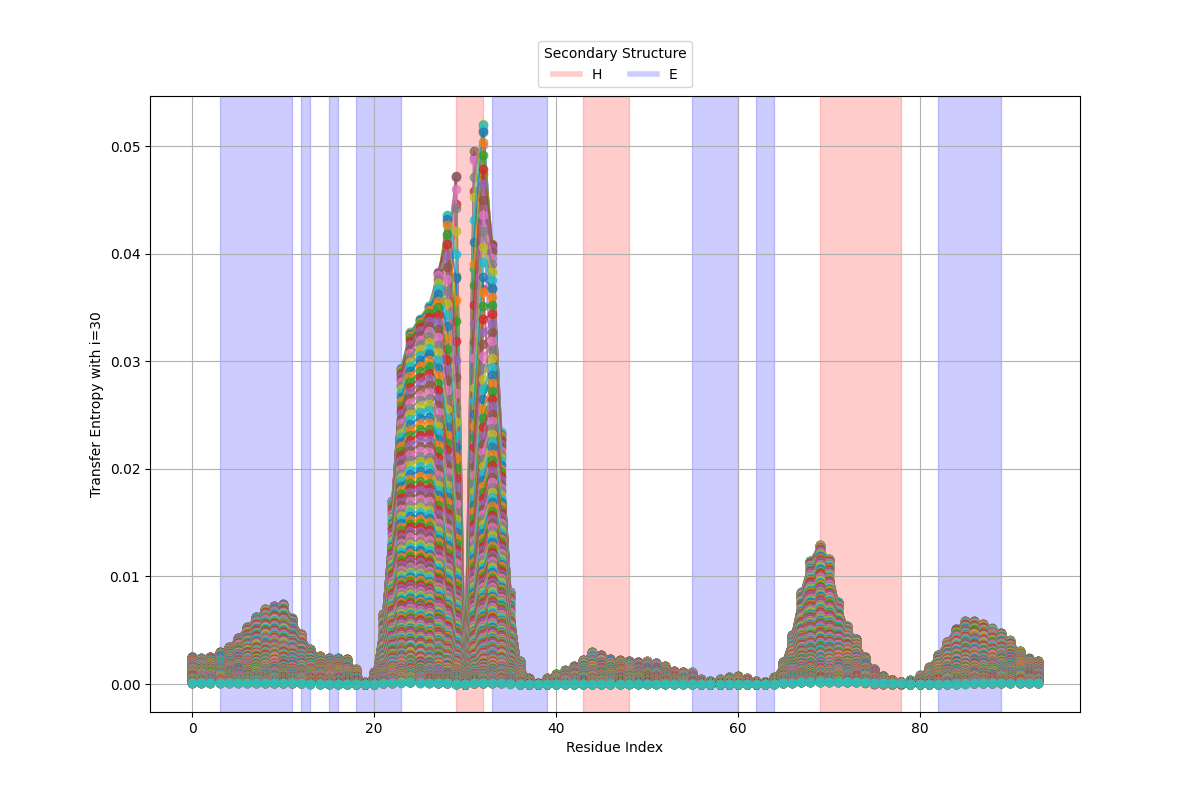
\includegraphics[width=0.8\textwidth]{/Users/enrico/PROTEINS/images/3LNX/Time_indicators/Transfer Entropy TE_ji for i=30 as a function of j at time index 0.png}
    \caption{Transfer Entropy 31->i (T_{i,31}).}
    \label{fig:TE31_pass}
\end{figure}
\begin{figure}[h!]
    \centering
    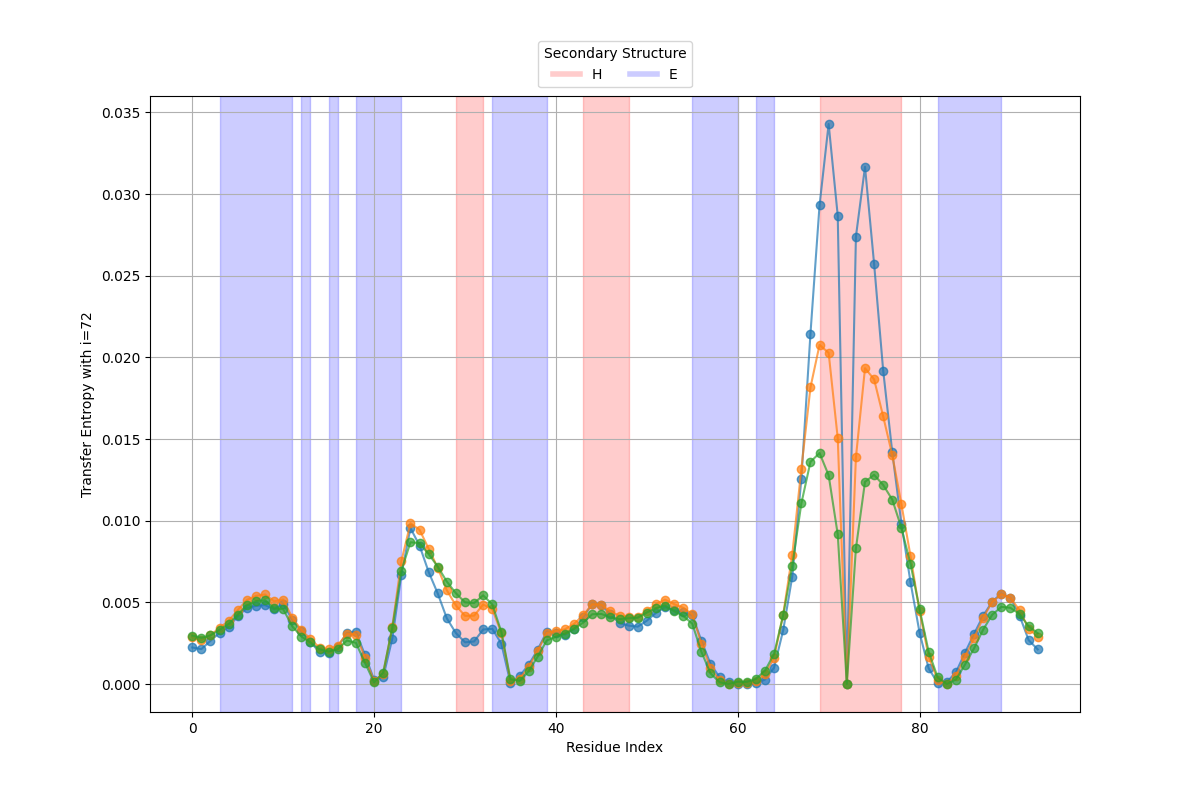
\includegraphics[width=0.8\textwidth]{/Users/enrico/PROTEINS/images/3LNX/Time_indicators/Transfer Entropy TE_ji for i=72 as a function of j at time index 0.png}
    \caption{Transfer Entropy 73->i (T_{i,73}).}
    \label{fig:TE73_pass}
\end{figure}
\newpage
In our analysis, we observed that we don't have a great difference in patterns between the active and passive transfer entropy.\\
Thus it suggest a bi-directional mechanism of action, so allosteric sites both influence and are influenced by the binding pocket within the protein.\\
Thus this dual role highlights the sophisticated nature of allosteric modulation, where sites are not merely passive receivers of signals but also react and comuniate with allsoteric sites.

\newpage
\newpage
\section{Conclusions of equlibrium stochastic process}
\noindent 
The findings presented in this chapter contribute significantly to our understanding of allosteric dynamics in proteins through the application of Gaussian network models and normal mode analysis.\\
The covariance matrices and beta factors revealed interaction patterns and mobility within protein structures that are crucial for biological function. \\
Notably, the identification of specific peaks in the beta factors corresponding to the binding pocket and allosteric sites suggests these areas could be critical for regulating protein activities.\\
Moreover, the comparison between experimental data and model predictions showed good agreement, indicating that the utilized models can effectively capture essential aspects of protein dynamics. \\
The behavior of the covariance matrices and response analysis highlighted how dynamical changes in one part of the protein can significantly influence other distance regions, suggesting allosteric behavior. \\
In addition the causal indicators between residues provided insights into the directional flow of information within the protein, revealing critical pathways of allosteric communication according to expected results.\\
These results align with the theoretical models discussed in previous chapters and provide empirical validation of our research hypotheses.\\
Thus these observations shed light on the functional interplay between the main secondary structural regions:  the binding pocket and the alpha helixs.\\
The analysis demonstrates that the geometric strucutrue of the protein is so important that is sufficent to explain mathematically the allosteric propagation of the protein.\\
So this method can be used to predict the allosteric sites of a protein and to understand the mechanism of the protein, helping the experimental biologysts to study allostery.\\
In addition this analysis suggest that not only there is a comunication between allosteric sites and active sites in protein, but also there is a comunication between allosteric sites.\\
Finaly this comunication between the allosteric sites and the binding pocket at equilibrium is reciprocal.\\
It would obviously be interesting to study the protein in out-of-equilibrium conditions to understand if the cause-effect behavior and the reciprocal communication between the allosteric sites and the binding pocket is still valid or if one will start to predominate over the other.

\newpage
\chapter{Out-of-Equilibrium Stochastic Processes Induced by Heat Gradients}
\noindent The first out-of-equilibrium condition for studying the protein is induced by a heat gradient.\\
In practice, what we will do is place the residues at two different temperatures based on their relative positions in the protein.\\
Infact it is imaginable that atoms inside the protein are more strongly bound and thus fluctuate less.\\
We introduced this heat gradient because we believe that allostery is often thought to emerge predominantly under non-equilibrium conditions.\\


\newpage
\section{Stochastic Dynamics Under a Heat Gradient}
\noindent In the equilibrium phase, as discussed in Chapter~\ref{sec:stochastic_processes}, the evolution of a system can be described by the following stochastic differential equation:
\begin{equation}
    \gamma \frac{d\mathbf{x}}{dt} = - g \mathbf{K} \mathbf{x} + \sqrt{2 \gamma k_B T} \boldsymbol{\eta}(t).
\end{equation}

In a system subjected to a heat gradient, the temperature varies spatially across the protein structure, with each residue experiencing a local temperature \( T(x) \) that depends on its position.
This introduces a non-equilibrium condition driven by spatially dependent thermal fluctuations.\\ 
Consequently, the motion equation is modified to account for this temperature gradient:
\begin{equation}
    \gamma \frac{d\mathbf{x(t)}}{dt} = - g \mathbf{K} \mathbf{x(t)} + \mathbf{B} \boldsymbol{\eta}(t).
\end{equation}
where \( B \) is a diagonal matrix that incorporates the temperature of each residue. Specifically, \( B = \sqrt{2 \gamma k_B T(x)} \), making the noise term position-dependent.\\ 
Applying a similar sostituion of the previous chapter, but this time writing the Hamiltonian in unit of $k_B$, the equation simplifies to:
\begin{equation}
    \frac{d\mathbf{x(t)}}{dt} = - g \mathbf{K} \mathbf{x(t)} + \mathbf{B} \boldsymbol{\eta}(t).
\end{equation}
where \( B \) is a diagonal matrix further refined to account for the discrete temperature values by incorporating a Kronecker delta function:\\
\begin{equation}
    B_{i,j}(x) = \delta_{i,j} \cdot \sqrt{T(x)}.
\end{equation}
This model enables a detailed exploration of the stochastic dynamics of proteins under non-equilibrium conditions.\\
Now we want to solve in the prevoius equation with the normal mode analysis so we can obtain the covariance function to analyze how the residues interact each other and we can obtain also the transfer entropy.\\
Substituting \(X(t) = \mathbf{V} \mathbf{Q}(t)\) in the motion equation, proceeding in the same way of the equilibrium case, we obtain:
\[
\frac{d(\mathbf{V} \mathbf{Q}(t))}{dt} = -g \mathbf{K} (\mathbf{V} \mathbf{Q}(t)) + \mathbf{B} \mathbf{\eta}(t).
\]
Substituting \(\mathbf{K} = \mathbf{V} \mathbf{\Lambda} \mathbf{V}^\top\), the term \(-\mathbf{K}(\mathbf{V} \mathbf{Q}(t))\) becomes:
\[
-\mathbf{K}(\mathbf{V} \mathbf{Q}(t)) = -\mathbf{V} \mathbf{\Lambda} \mathbf{V}^\top (\mathbf{V} \mathbf{Q}(t))= - \mathbf{V} \mathbf{\Lambda} \mathbf{Q}(t)..
\]
Thus the equation becomes:
\[
\mathbf{V} \frac{d\mathbf{Q}(t)}{dt} = - g \mathbf{V} \mathbf{\Lambda} \mathbf{Q}(t) + \mathbf{B} \mathbf{\eta}(t).
\]
Multiplying both sides by \(\mathbf{V}^\top\) (to return to the eigenvector space):
\[
\frac{d\mathbf{Q}(t)}{dt} = - g \mathbf{\Lambda} \mathbf{Q}(t) + \mathbf{V}^\top \mathbf{B} \mathbf{\eta}(t).
\]
So for each component \(i\), we have:
\[
\frac{dQ_{i}(t)}{dt} = - g \lambda_i Q_{i}(t) + \sum_j v_{ji}^\top B_{jj} \eta_{j}(t).
\]
As in the equilibrium case, the deterministic term \(-\lambda_i Q_{i}(t)\) describes the evolution of the components \(Q_{i}(t)\) under the influence of the eigenvalue \(\lambda_i\), instead the stochastic term \(\sum_j v_{ji}^\top B_{jj} \eta_{j}(t)\) represents the effect of noise transformed in the eigenvector space.\\
The solution is:
\[
Q_{i}(t) = \int_{-\infty}^t e^{- g \lambda_i (t - \tau)} \sum_j v_{ji}^\top B_{jj} \eta_{j}(\tau) \, d\tau.
\]
We now compute the Covariance between normal modes:
\[
\langle Q_i(t) Q_j(s) \rangle = \left\langle \int_{-\infty}^t e^{- g \lambda_i (t - \tau)} \sum_k v_{ki}^\top B_{kk} \eta_{k}(\tau) \, d\tau \, \int_{-\infty}^s e^{- g \lambda_j (s - \tau')} \sum_l v_{lj}^\top B_{ll} \eta_{l}(\tau') \, d\tau' \right\rangle.
\]
Expanding, we get:
\[
\langle Q_i(t) Q_j(s) \rangle = \int_{-\infty}^t \int_{-\infty}^s e^{- g \lambda_i (t - \tau)} e^{- g \lambda_j (s - \tau')} \sum_k \sum_l v_{ki}^\top B_{kk} v_{lj}^\top B_{ll} \langle \eta_{k}(\tau') \eta_{l}(\tau') \rangle \, d\tau \, d\tau'.
\]
The noise term \(\langle \eta_{k}(\tau) \eta_{l}(\tau) \rangle\) satisfies:
\[
\langle \eta_{k}(\tau) \eta_{l}(\tau') \rangle = \delta_{kl} \delta(\tau - \tau'),
\]
which simplifies the double integral:
\[
\langle Q_i(t) Q_j(s) \rangle = \sum_k (v_{ki}^\top B_{kk}) (v_{kj}^\top B_{kk}) \int_{-\infty}^{min(t,s)} e^{-g \lambda_i (t - \tau)} e^{-g \lambda_j (s - \tau)} \, d\tau.
\]
Evaluating the integral:
\[
\int_{-\infty}^{min(t,s)} e^{-g(\lambda_i t + \lambda_j s)} e^{g(\lambda_i + \lambda_j) \tau} \, d\tau = \frac{e^{-g(\lambda_i t + \lambda_j s)}}{g(\lambda_i + \lambda_j)} \left[ e^{g(\lambda_i + \lambda_j) min(t,s)} \right].
\]
So finally we obtain:
\[
\langle Q_i(t) Q_j(s) \rangle = \sum_k \frac{(v_{ki}^\top B_{kk}) (v_{kj}^\top B_{kk})}{g(\lambda_i + \lambda_j)} e^{-g\lambda_i |t-s|}.
\]
Now we can caompute teh covariance easily in the original space:
\[
\langle X_i(t) X_j^\top(s) \rangle = \sum_k \sum_p \sum_m \frac{v_{ik} v_{jp} (v_{mk}^\top B_{mm}^2 v_{mp}^\top)}{g(\lambda_k + \lambda_p)} e^{-g \lambda_k |t-s|}.
\]
The formula describes the temporal Covariance between the components \( X_i(t) \) and \( X_j(s) \) in a stochastic system under the influence of noise and a gradient of temperature. \\
Analyzing the formula we have the eigenvectors (\( v_{ik} \) and \( v_{jp} \)). Their role is to write the Covariance in the eigenbasis of the matrix \( {K} \). Instead the diagonal matrix \( B_{mm}^2 \) is the fundamental term becasue it introduces the dependence from the temperature and thus the non equilibrium.
Finally the term \( e^{-g \lambda_k |t-s|} \) encapsulates the temporal decay of the Covariance, governed by the eigenvalue \( \lambda_k \), more the eigenvalues are larger,  faster the covariance decays.\\ 
The non equilibrium is also highlighted by the fact that the covariance is no more simmetric in time, suggesting a precise information direction. \\
The denominator ensures that the contributions from eigenmodes are properly weighted by their respective damping rates \( \lambda_k \) and \( \lambda_p \).
As before the transfer entropy it is completely determined by the Covariance.
Otherwise define the linear response out of equilibrium is not easy, however is not our aim.


\newpage
\section{Temperature determination}
\noindent As we said, we set two distinct temperature regimes.\\
One temperature is fixed at \( T = 1 \), representing a high-energy state, while the other temperature varies between \( T = 0 \) and \( T = 1 \) for each experiment, so it is \( T = 1 - \epsilon,\),
where \( \epsilon = \{1.0, 0.9, 0.8, 0.7, 0.6, 0.5, 0.4, 0.3, 0.2, 0.1, 0.0\} \) for a total of 11 experiments (Note that when  \( epsilon = 0 \) we are in the equilibrium case as before, so the results must be the same).\\
This configuration allows us to drive the system out of equilibrium and study the allosteric behavior under non-equilibrium conditions.\\
The temperature assigned to a given residue is determined based on its connectivity within the protein structure. Specifically, if a residue has five or more connections, it is assigned a temperature of \( T = 1 - \epsilon,\)  (varying temperature);
otherwise, it is assigned \( T = 1 \). This methodology links the temperature directly to the residue's position and role within the protein network.\\
Residues located near the center of the protein typically exhibit a higher number of connections due to their central role in maintaining structural integrity.\\
These residues tend to fluctuate less and are therefore associated with lower effective temperatures. \\
Conversely, residues with fewer connections, often found on the periphery, are more flexible and are assigned higher temperatures.\\
\begin{figure}[h!]
    \centering
    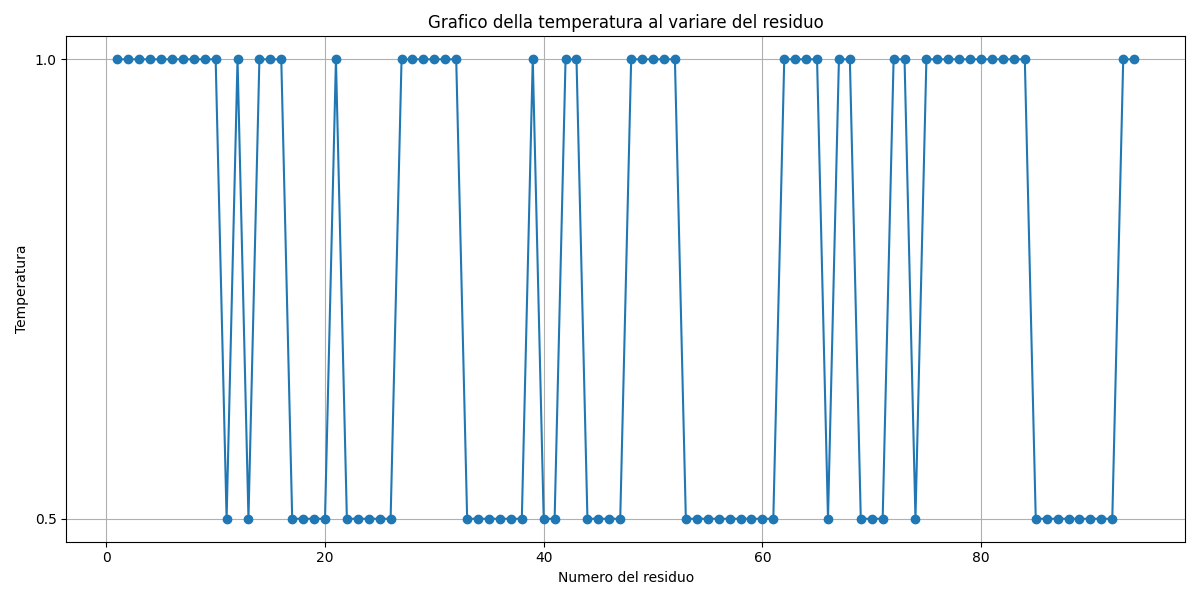
\includegraphics[width=0.8\textwidth]{/Users/enrico/PROTEINS/images/3LNX/2_temperature_cutoff/temperatures.png}
    \caption{Temperature vs residue number}
    \label{fig:Temperature vs residue number}

\end{figure}
In the images \ref{fig:Temperature vs residue number} we have a represention of the different temperatures of every residues.\\
What we can see is that in the beta sheet regions residues tend to have higher connectivity due to their compact and stabilizing arrangement in the protein's core, otherwhise in the Alpha helix regions typically exhibit intermediate levels of connectivity.\\
Finally residues located in loops or on the protein's surface generally have fewer connections, as these regions are more exposed and less structurally integrated.\\
now that we hace a deeper understanding of the non equilibrium condition we are ready to compute and anlyze the allostery through the causal indicators.\\

\newpage

\chapter{Results of the non equilibrium dynamic}
\noindent In this chapter we will expose the results obtain for the non-equilibrium stochastic process describing the oscilaltions of atoms in the protein under a heat gradient.\\
We will compare the results with the equilibrium case to see how the heat gradient affects the protein.\\
For the connection radius and for the Kirchhoff matrix are valid the precedence arguments in section \ref{Kirchhoff_paragraph}.\\
Moreover we used the same characteristic time finded in the equilibrium case.\\
First we will describe the covariance and the beta factors to evaluate the quality of the model and after we will check how the heat gradient affects the protein's allosteric mechanism.\\

\section{Covariance Matrix and Beta Factors}
\noindent 
Let's start by analyzing the Covariance matrices obtained from the non-equilibrium stochastic process compared to the equlibrium case.\\
\begin{figure}[h!]
    \centering
    \begin{minipage}{0.49\textwidth}
        \centering
        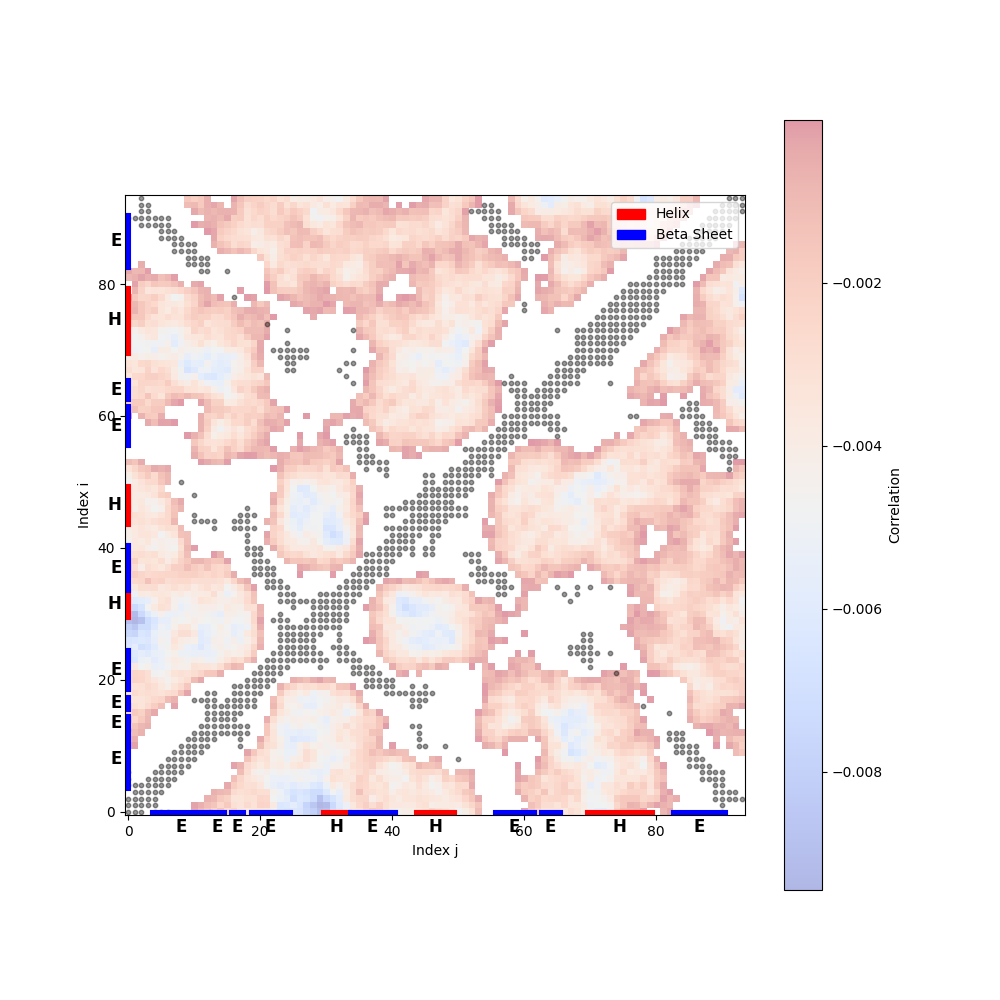
\includegraphics[width=\textwidth]{/Users/enrico/PROTEINS/images/3LNX/2_temperature_cutoff/Matrici_Correlazione/Correlation_MatrixNan_False_0.2.png}
        \caption{Negative covariance between residues at time 0 with \( T = 1-\epsilon = 0.2\).}
    \end{minipage}
    \hfill
    \begin{minipage}{0.49\textwidth}
        \centering
        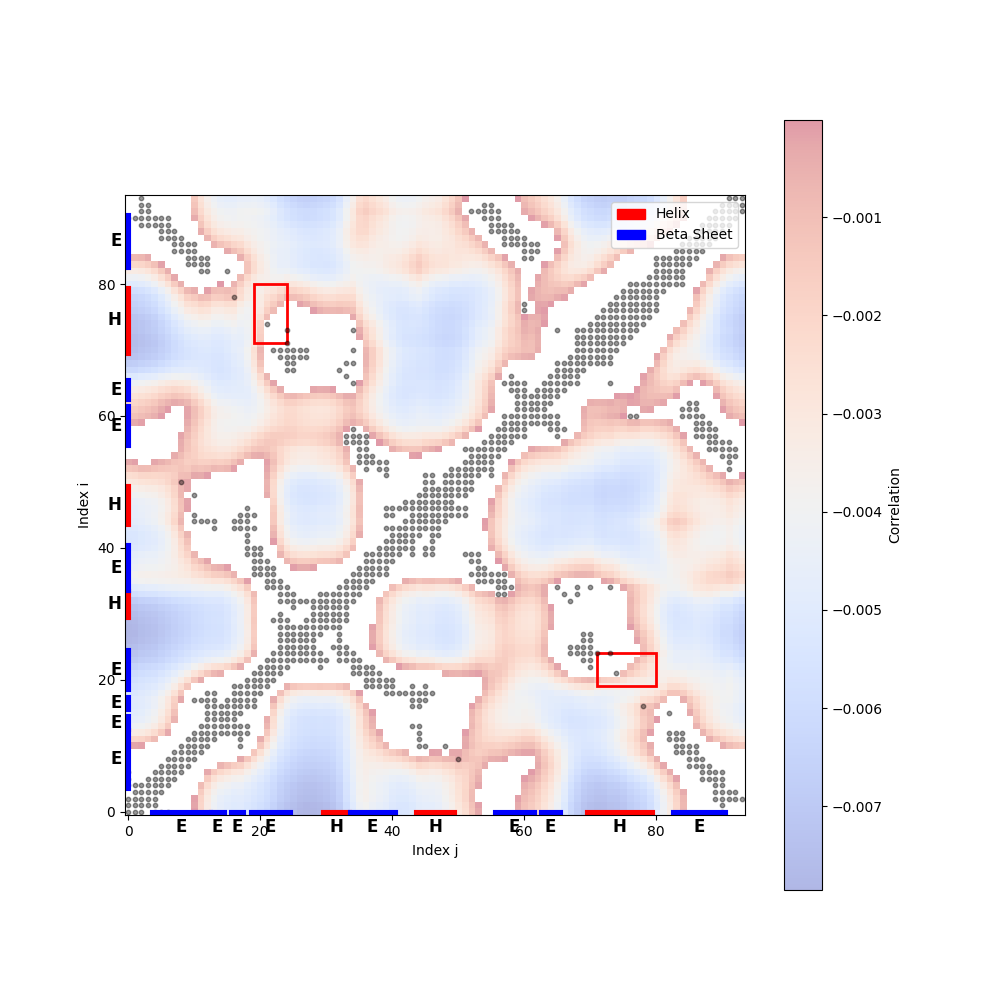
\includegraphics[width=\textwidth]{/Users/enrico/PROTEINS/images/3LNX/2_temperature_cutoff/Matrici_Correlazione/Correlation_MatrixNan_False_1.png}
        \caption{Negative covariance between residues at time 0 with \( T = 1-\epsilon =1\) (equilibrium case).}
    \end{minipage}
    \caption{Comparison of negative covariances between residues at time 0 for different $T$ values.}
    \label{fig:Covariance_comparison_out}
\end{figure}
In the image \ref{fig:Covariance_comparison_out}, we observe the negative part of the Covariance matrix at two different temperature settings:
The left matrix (\( T = 1-\epsilon = 0.2\)) shows localized and intense negative covariance clusters confronting to the equilibrium covariance matrix.\\
This finer detail indicates that at lower temperatures, the protein's structural elements are less mobile, leading to more pronounced and localized interactions between residues.\\
This seems coherent.\\
In contrast, the right matrix (\( T = 1-\epsilon =1\) (equilibrium case)) exhibits smoother covariance patterns, which suggests increased mobility of the residues in a disordered way.\\
At this equilibrium temperature, the increased thermal energy allows for greater mobility of the protein's residues, smoothing out the localized negative covariance patterns seen at lower temperatures.\\
This enhanced flexibility can be advantageous for proteins that need to adapt to different functional states or interact with various molecular partners.\\
Obviously at higher temperatures, the smooth patterns suggest that the residues are moving more freely, reflecting increased kinetic energy.\\
This flexibility allows proteins to adapt their shapes more readily, accommodating various biochemical interactions required for cellular processes.\\
The ability to adjust structure with temperature facilitates essential functions such as substrate binding in enzymes.\\

\newpage
\begin{figure}[h!]
    \centering
    \begin{minipage}{0.49\textwidth}
        \centering
        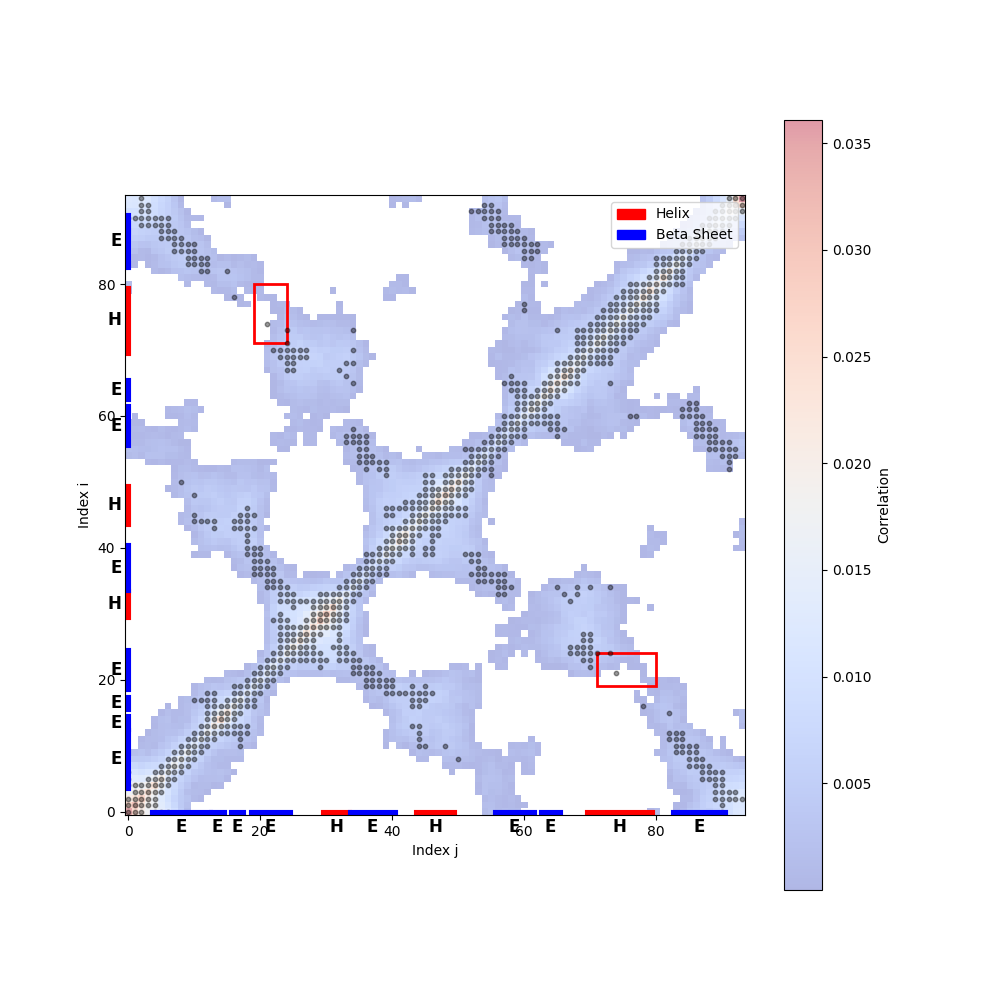
\includegraphics[width=\textwidth]{/Users/enrico/PROTEINS/images/3LNX/2_temperature_cutoff/Matrici_Correlazione/Correlation_MatrixNan_True_0.2.png}
        \caption{Positive covariance between residues at time 0 with \( T = 1-\epsilon = 0.2\).}
        
    \end{minipage}
    \hfill
    \begin{minipage}{0.49\textwidth}
        \centering
        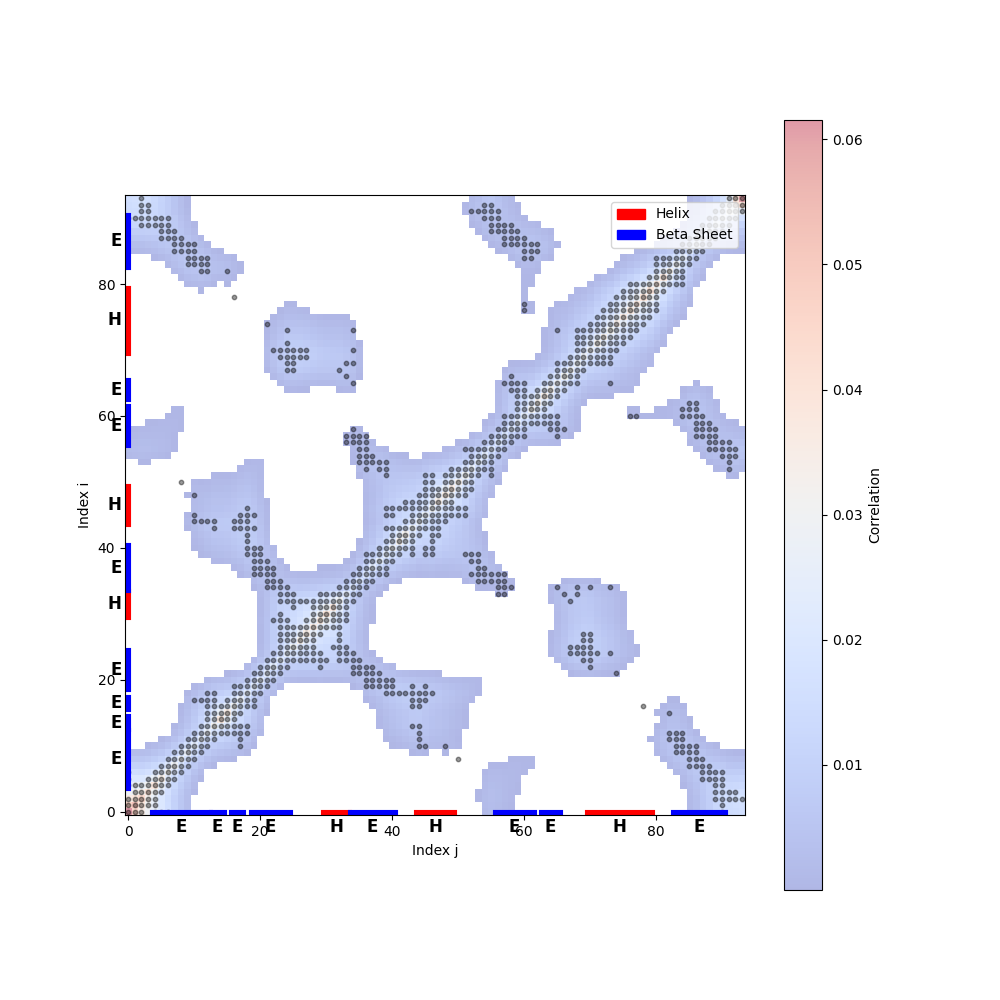
\includegraphics[width=\textwidth]{/Users/enrico/PROTEINS/images/3LNX/2_temperature_cutoff/Matrici_Correlazione/Correlation_MatrixNan_True_1.png}
        \caption{Positive covariance between residues at time 0 with \( T = 1-\epsilon =1\) (equilibrium case).}
        
    \end{minipage}
    \caption{Comparison of positive covariances between residues at time 0 for different $ T$ values.}
    \label{fig:Covariance_positive_comparison_out}
\end{figure}

Instead the image \ref{fig:Covariance_positive_comparison_out} represents the positive part of the Covariance matrix at two different temperatures and the analysis is the viceversa of the previous case:
At \( T = 1-\epsilon = 0.2\), the Covariance patterns are more sparse and lower.\\
This localization suggests that at lower temperatures, protein structures are more rigid and interactions between residues are more specific, potentially stabilizing certain functional forms or interactions essential for biological activity in colder environments.\\
instead at \( T = 1-\epsilon =1\)(equilibrium case), the Covariances are more localized, suggesting increased flexibility.\\


\newpage
Now that we have the covariance matrix we can calculate the beta factors to evaluate the quality of the model.\\
The plot above compares the experimental \( B \)-factors (blue curve), represented by the formula \eqref{beta} $B_i = 8\pi^2 C_{ii}$, with the predicted \( B \)-factors (red curve) along the residue index. \\
These metrics provide a quantitative assessment of the model's accuracy in capturing the protein's dynamic behavior, revealing how well the theoretical models approximate realresidues vibrations.
\begin{table}[ht]
    \centering
    \begin{tabular}{|c|c|c|}
        \hline
        $\Delta T$ & MAE & RMSE \\ \hline
        $T=1$ & 6.4146 &  8.5200 \\ \hline
        $T=0.9$ & 6.3206 &  8.4244 \\ \hline
        $T=0.8$ & 6.2239 &  8.3239 \\ \hline
        $T=0.7$ & 6.1239 &  8.2191 \\ \hline
        $T=0.6$ & 6.0212 &  8.1107 \\ \hline
        $T=0.5$ & 5.9457 &  8.0004 \\ \hline
        $T=0.4$ & 5.8701 &  7.8913 \\ \hline
        $T=0.3$ & 5.8117 &  7.7885 \\ \hline
        $T=0.2$ & 5.7542 &  7.7003 \\ \hline
        $T=0.1$ & 5.7030 &  7.6413 \\ \hline
        $T=0.0$ & 5.6775 &  7.6319 \\ \hline
    \end{tabular}
    \caption{Errors of MAE and RMSE for different values of $\Delta T$}
    \label{tab:mae_rmse}
\end{table}

\begin{figure}[h!]
    \centering
    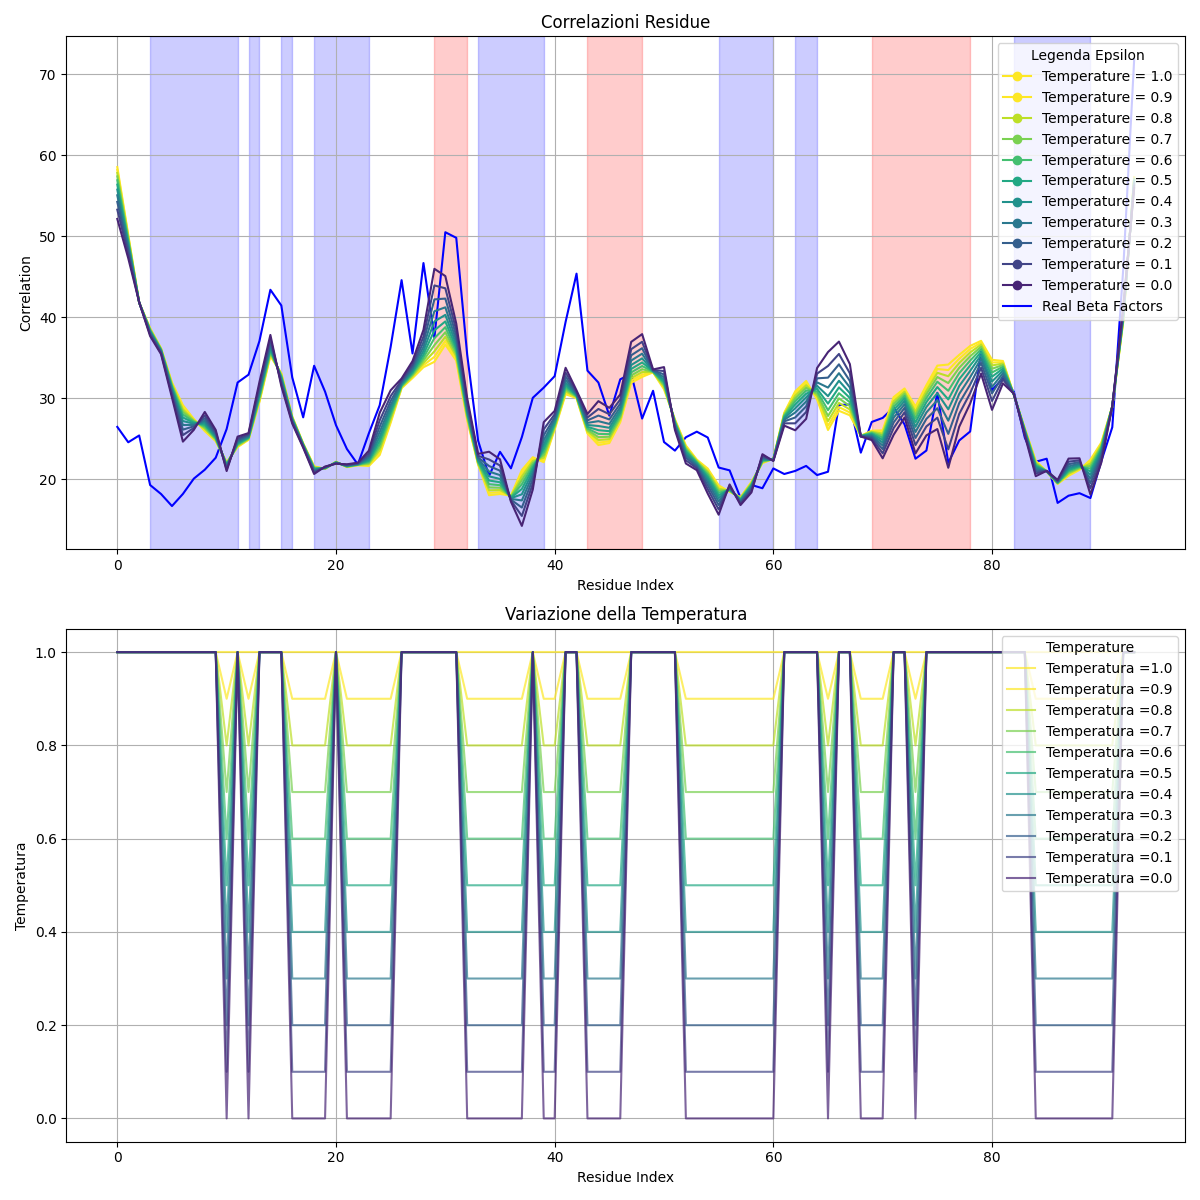
\includegraphics[width=0.8\textwidth]{/Users/enrico/PROTEINS/images/3LNX/2_temperature_cutoff/beta_factors/beta.png}
    \caption{Beta factors with different $\Delta T$.}
\end{figure}
By analyzing the system in and out of equilibrium \(\Delta T = 1 - \epsilon \), we observe that the system driven out of equilibrium (\(\Delta T = 1\)) fits better the beta factors, resulting in lower error metrics and better alignment between predicted and experimental \( B \)-factors. \\
This indicates that the system's response to a larger temperature gradient is more realistic and so also the real world protein exhibits different intensity in the fluctuations of its atom internally and externally.\\
In particular now we can catch in a better way the spikes around the $alpha-\alpha$ and around the end of $alpha-\beta$ and  $alpha-\gamma$ helixs\\
In conclusion the out of equilibrium model is a better approximation of the real protein's behavior.\\

\newpage


\section{Causal indicators between residues}
\noindent In this section our aim is to understand how the out of equilibrium condition affects the causal allosteric relationship between residues.\\
We will anlyze the covariance and the transfer entropy between residues, confronting the results with the equilibrium condition.\\
It is interesting to see how the heat gradient affects the signal propagation in the protein and if the reciprocal mechanism of allostery find in the equilibrium case is still valid.\\
Let's start with the covariance between the residues: We want to see, as before, a high absolute value of covariance between the allosteric sites and the active sites in the binding pocket.\\


\begin{figure}[h!]
    \centering
    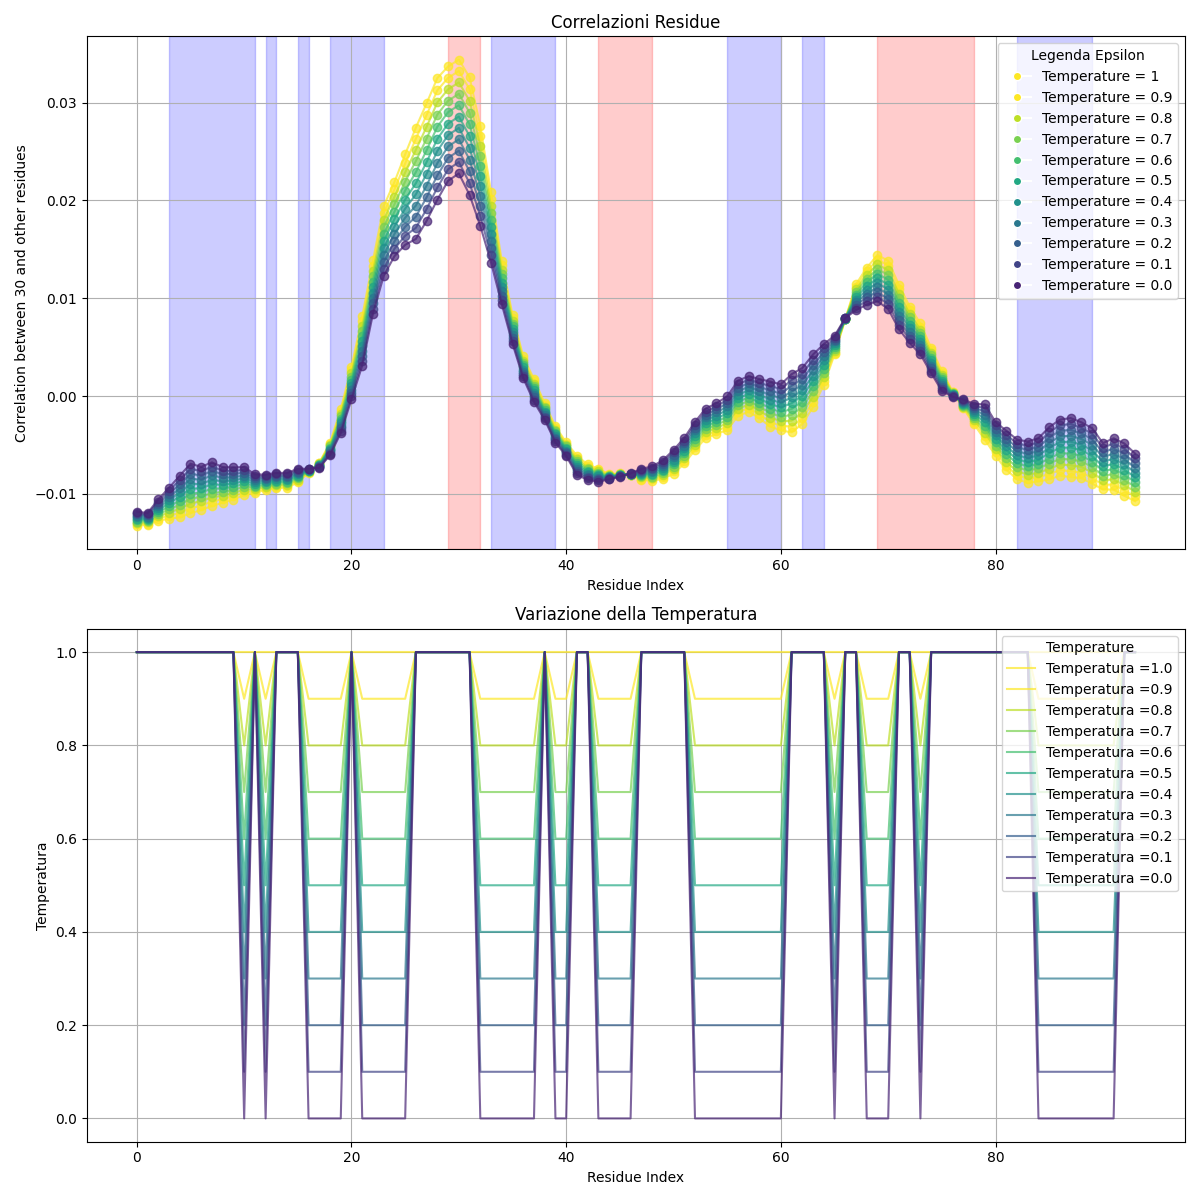
\includegraphics[width=0.8\textwidth]{/Users/enrico/PROTEINS/images/3LNX/2_temperature_cutoff/combined_correlation_30_temperature_plots.png}
    \caption{Dynamic covariance observed from perturbating the 31-th residue, illustrating signal propagation through alpha-$alpha$ helical regions out of equilibrium.}
    \label{fig:corr31_out}
\end{figure}
Analyzing figure \ref{fig:corr31_out} we notice that are valid the conclusion of the equilibrium part, as we said:
There are a high Covariance observed near the binding pocket,as we expected, particularly between the alpha-$\alpha$ and beta-$\beta$ regions, and another allosteric site in the alpha-$\gamma$ helix, highlights regions of significant allosteric communication.\\
Moreover we see also strong values of covariance in the head and in the tail of the protein, probability caused by spourious interactions. 
\newpage
\begin{figure}[h!]
    \centering
    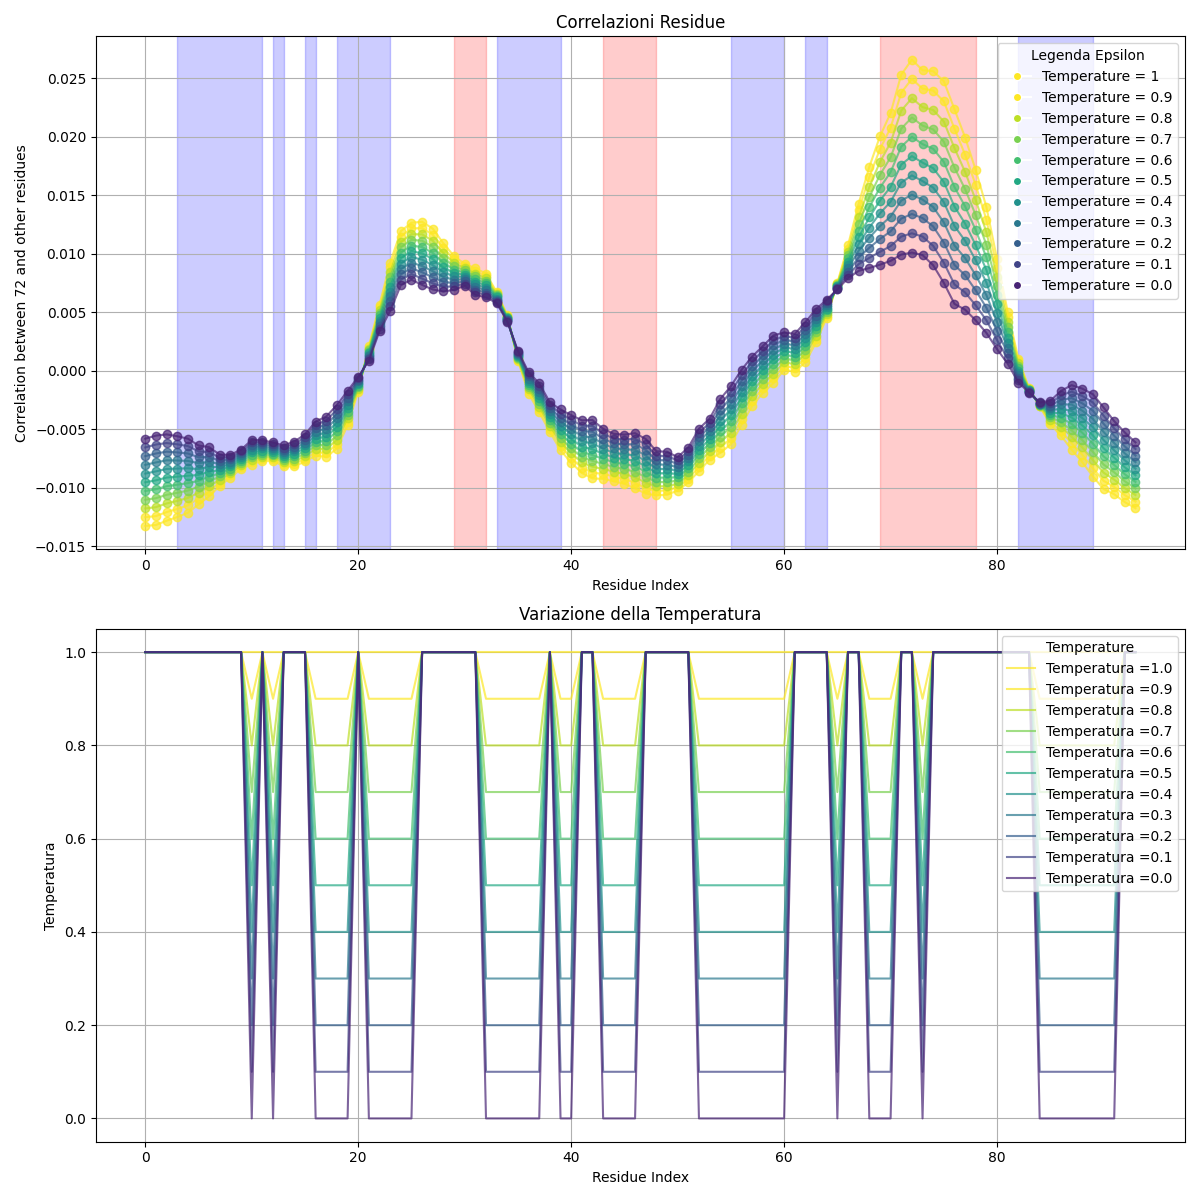
\includegraphics[width=0.8\textwidth]{/Users/enrico/PROTEINS/images/3LNX/2_temperature_cutoff/combined_correlation_72_temperature_plots.png}
    \caption{Dynamic covariance observed from perturbating the 73-rd residue, illustrating signal propagation through alpha-$gamma$ helical regions out of equilibrium.}
    \label{fig:corr73_out}
\end{figure}
Also for the Covariance of residue 73 \ref{fig:corr73_out} the general conclusion is still the same of the equilibrium case.\\


Moreover for both the images when temperatures are higher we can see how more dispersed and higher in modulus the covariance is.\\
Instead at lower temperatures the covariance is more localized.\\
Especially we see a lot of variance of the correlation in function  of the temperature around the alpha-$\alpha$-helix.\\
We can also see that the covariance for some residues are completely indifferent to the heat gradient.\\
Finally we see also that the values of the covariance when we introduce the gradient not become all higher o lower but some become higher and some other lower.\\
In conclusion the allosteric behavior in the covariances of the protein is the same of the equilibrium case but the model explain in a better way the beta factors.\\


\newpage
\begin{thebibliography}{100}

    \bibitem{ref} 
    \url{https://www.sciencelearn.org.nz/resources/209-role-of-proteins-in-the-body}
    
    \bibitem{ref2} 
    \emph{University of California Davis, Introductory Biology}, 
    \url{https://bio.libretexts.org/Courses/University_of_California_Davis/BIS_2A%3A_Introductory_Biology_%28Easlon%29/Readings/04.3%3A_Amino_Acids}
    
    \bibitem{ref3} 
    \emph{University of California Davis, Introductory Biology}, 
    \url{https://bio.libretexts.org/Courses/University_of_California_Davis/BIS_2A%3A_Introductory_Biology_%28Britt%29/01%3A_Readings/1.17%3A_Protein_Structure}
    
    \bibitem{ref4} 
    Nature, \url{https://www.nature.com/scitable/topicpage/protein-structure-14122136/}
    
    \bibitem{ref5} 
    Wikipedia, Allosteric regulation 
    
    \bibitem{ref6} 
    Statistical Mechanics of Allosteric Enzymes
    
    \bibitem{ref7} 
    University of California Davis, Introductory Biology, Hemoglobin and allosteric effects
    
    \bibitem{ref8} 
    Allosterism in the PDZ Family, Amy O. Stevens and Yi He
    
    \bibitem{ref9} 
    Protein elastic network models and the ranges of cooperativity, Lei Yanga, Guang Songa, and Robert L. Jernigana
    
    \bibitem{ref11} 
    Introduzione alla Teoria dei Grafi, Vittorio Loreto, Francesca Tria.
    
    \bibitem{ref12} 
    Time and ensemble-average statistical mechanics of the Gaussian network model, Alessio Lapolla, Maximilian Vossel, and Aljaz Godec
    
    \bibitem{ref13} 
    Covariance, response and entropy approaches to allosteric behaviors: a critical comparison on the ubiquitin case Fabio Cecconi, Giulio constantini, Carlo Guardiani, Marco Baldovin and Angelo Vulpiani
    
    \bibitem{ref14} 
    Robust inference of causality in high-dimensional dynamical processes from the Information Imbalance of distance ranks
    Vittorio Del Tatto, Gianfranco Fortunato, Domenica Bueti, and Alessandro Laio
    
    \bibitem{ref15} 
    Allosterism in the PDZ Family, Amy O. Stevens and Yi He.

    
\end{thebibliography}

\end{document}















\subsubsection{Temperature Variation and General Observations}
\begin{itemize}
    \item \textbf{Temperature Oscillations:} Both figures show regular oscillations in temperature, reflecting dynamic structural changes in the protein.
    \item \textbf{Flexibility vs. Rigidity:} High temperatures (\( T = 1.0 \)) are associated with broader fluctuations and more dispersed Covariance effects, while low temperatures (\( T = 0.0 \)) correspond to sharp, localized peaks, indicating more rigid and limited dynamic behavior.
\end{itemize}


\subsubsection{Conclusions}











\newpage
\newpage


\begin{figure}[htbp]
    \centering
    % Prima sottografia
    \begin{subfigure}[t]{0.45\textwidth}
        \centering
        \includegraphics[width=\textwidth]{/Users/enrico/PROTEINS/CUTOFF/images/3LNX/2(t)emperature_cutoff/combined_entropy(t)emperature_20_plots.png}
        \caption{Transfer Entropy ($TE_{21,j}$) perturbating the 21st residue.}
        \label{fig:TE21_i_j_out}
    \end{subfigure}
    \hfill
    % Seconda sottografia
    \begin{subfigure}[t]{0.45\textwidth}
        \centering
        \includegraphics[width=\textwidth]{/Users/enrico/PROTEINS/CUTOFF/images/3LNX/2(t)emperature_cutoff/combined_entropy(t)emperature_75_plots.png}
        \caption{Transfer Entropy ($TE_{76,j}$) perturbating the 76th residue.}
        \label{fig:TE76_i_j_out}
    \end{subfigure}
    % Didascalia principale
    \caption{Comparison of Transfer Entropy for different perturbed residues.}
    \label{fig:TE_comparison_i_j_out}
\end{figure}


\subsection{Conclusion}
The analysis reveals that driving the system out of equilibrium (\(\Delta T = 1\)) results in lower MAE and RMSE values and better alignment between predicted and experimental \( B \)-factors. Non-equilibrium conditions create more structured and predictable dynamics, while closer-to-equilibrium systems (\(\Delta T = 0.5\)) exhibit subtler and more stochastic flexibility patterns. These findings underscore the stabilizing effect of non-equilibrium conditions on protein dynamics and highlight the critical role of temperature gradients in studying and modeling protein flexibility.




\newpage
\section{Causal between residues}
\noindent Now we will see the cross covariance in time and the transfer entropy in time.\\
We will attend a non simmetric funcitonal form backward and forward.



\subsection{Cross covariance in time}
\begin{figure}[h!]
    \centering
    \includegraphics[width=0.8\textwidth]{/Users/enrico/PROTEINS/images/3LNX/2_temperature_cutoff/Time_Covariances/Covariance_combined.png}
    \caption{Covariance in time $\Delta T = 1$.}
\end{figure}
\noindent  Let’s start with the covariance in time, as we said before the Covariance is defined
as:
\[
\langle X_i(t) X_j^\top(s) \rangle = \sum_k \sum_p \sum_m \frac{v_{ik} v_{jp} (v_{mk}^\top B_{mm}^2 v_{mp}^\top)}{\lambda_k + \lambda_p} e^{-g \lambda_k |t-s|}.
\]
This behavior is coherent with what expected, the Covariance decay over time,indicating a loss of direct dynamic influence as time progresses.
Moreover Covariance values vary significantly between residue pairs, reflecting
differences in their initial dynamic coupling.\\
In additon out of equilibrium we can see that the cross-covariance is not time simmetric, in fact the forward covaraince is different from the backward.\\

\newpage
\subsection{Transfer Entropy: Forward and Backward Dynamics}
\begin{figure}[h!]
    \centering
    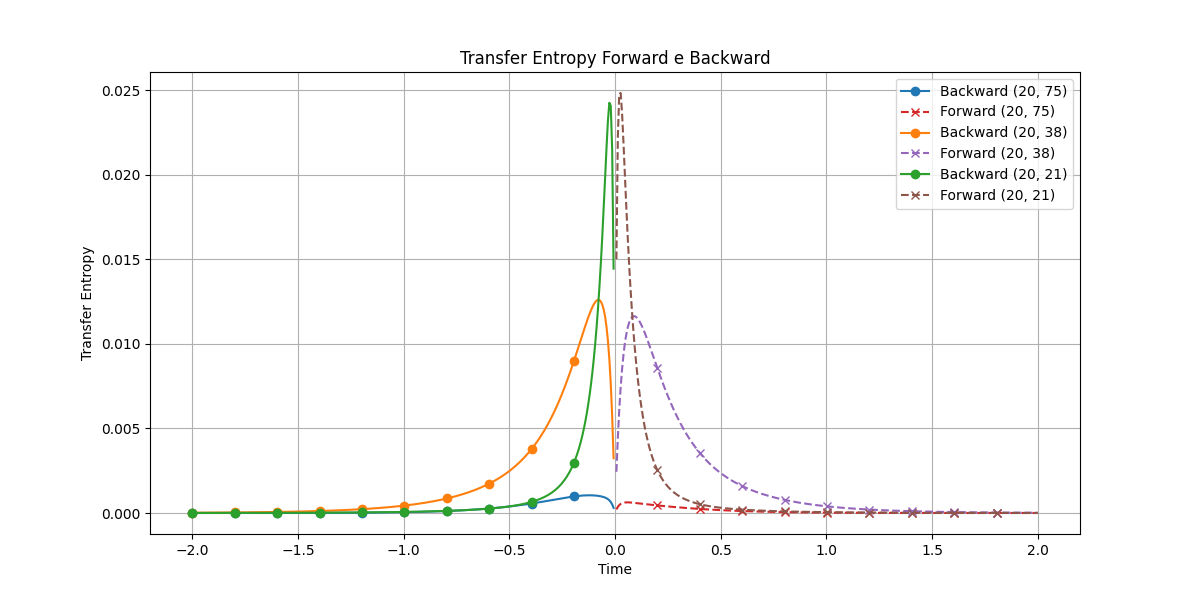
\includegraphics[width=0.8\textwidth]{/Users/enrico/PROTEINS/images/3LNX/2(t)emperature_cutoff/Time_Covariances/entropies_combined.png}
    \caption{Transfer entropy in time $\Delta T = 1$.}
\end{figure}

\noindent Also here, Obviosly, the transfer entropy is not time simmetric.\\
In addition the equilibrium reaseasons are valid: We see that a peak is observed at an intermediate time point for
most residue pairs, indicating a time of maximum information transfer.

\newpage
\section{Causal indicators between residues}
In this section our aim is to understand how the out of equilibrium condition affects the causal allosteric relationship between residues.\\
We will anlyze the covariance and the transfer entropy between residues, confronting the results with the equilibrium condition.\\
It is interesting to see how the heat gradient affects the signal propagation in the protein.\\


\newpage

\noindent 


When temperatures are higher we can see how more dispersed and higher in modulus the Covariance are.\\
Instead at lower temperatures the Covariance are more localized.\\
We can alsoo see that the covariance for some residues are completely indifferent to the heat gradient.\\ 









\subsubsection{Conclusions}











\newpage
\newpage


\begin{figure}[htbp]
    \centering
    % Prima sottografia
    \begin{subfigure}[t]{0.45\textwidth}
        \centering
        \includegraphics[width=\textwidth]{/Users/enrico/PROTEINS/CUTOFF/images/3LNX/2_temperature_cutoff/combined_entropy(t)emperature_20_plots.png}
        \caption{Transfer Entropy ($TE_{21,j}$) perturbating the 21st residue.}
        \label{fig:TE21_i_j_out}
    \end{subfigure}
    \hfill
    % Seconda sottografia
    \begin{subfigure}[t]{0.45\textwidth}
        \centering
        \includegraphics[width=\textwidth]{/Users/enrico/PROTEINS/CUTOFF/images/3LNX/2t)emperature_cutoff/combined_entropy(t)emperature_75_plots.png}
        \caption{Transfer Entropy ($TE_{76,j}$) perturbating the 76th residue.}
        \label{fig:TE76_i_j_out}
    \end{subfigure}
    % Didascalia principale
    \caption{Comparison of Transfer Entropy for different perturbed residues.}
    \label{fig:TE_comparison_i_j_out}
\end{figure}


\subsection{Conclusion}
The analysis reveals that driving the system out of equilibrium (\(\Delta T = 1\)) results in lower MAE and RMSE values and better alignment between predicted and experimental \( B \)-factors. Non-equilibrium conditions create more structured and predictable dynamics, while closer-to-equilibrium systems (\(\Delta T = 0.5\)) exhibit subtler and more stochastic flexibility patterns. These findings underscore the stabilizing effect of non-equilibrium conditions on protein dynamics and highlight the critical role of temperature gradients in studying and modeling protein flexibility.

